\pagebreak
\thispagestyle{empty}

\begin{center}
\begin{figure}[H]
\begin{absolutelynopagebreak}
  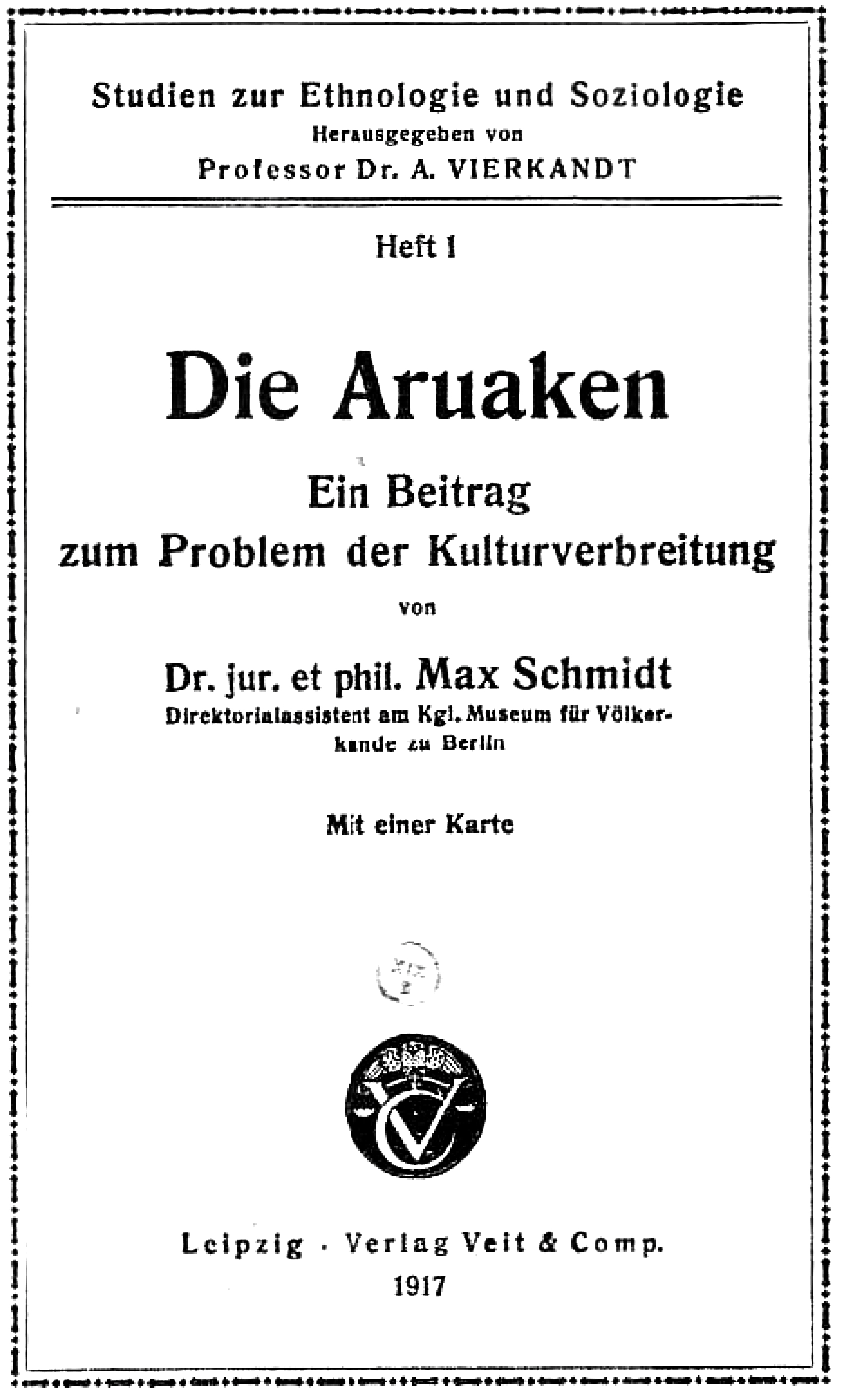
\includegraphics[width=\textwidth]{./FRONTISPICIO.pdf}  
  %\hfill
 % \caption{Frontispício da primeira edição.}

\end{absolutelynopagebreak}
\end{figure}
\end{center}

\part{Os Aruaques}
%{\textsc{os aruaques\\uma contribuição\\ para o problema da difusão cultural}}
\pagestyle{baruch}

\chapter*{Primeiras considerações\smallskip\subtitulo{Considerações metodológicas\\preliminares}}
\markboth{Primeiras considerações}{}
\addcontentsline{toc}{chapter}{Primeiras considerações}

Múltiplas são as tarefas da antropologia, e igualmente múltiplos são os
métodos para se aproximar gradualmente da solução destas tarefas. Desde
o desabrochar dessa jovem ciência nas últimas décadas, os seus problemas
e sucessos foram cada vez mais incluídos nos domínios de outras ciências
análogas, as quais, como ela, aspiram em sua elevada finalidade última,
ao registro universal das diferentes manifestações da humanidade e de
seu desenvolvimento, seja como fim em si mesma, seja como meio para o
progresso das tarefas culturais humanas em fundamentos científicos. Não
se considera mais apenas as qualidades da etnologia como disciplina
autônoma, mas ela também se tornou uma ciência auxiliar das ciências
históricas, da psicologia, das ciências da religião, da jurisprudência
e principalmente também da sociologia, com seu ramo principal, a
economia nacional. Isso lhe provém exigências completamente novas,
especialmente nos aspectos sistemáticos. Para ela, estas exigências se
consideram quanto ao método e à elaboração sistemática, frequentemente
antecipando amplos rumos científicos, não mais apenas como meio
auxiliar para o estímulo de novas perguntas ou para exposição de novos
métodos. Ela não pode mais construir seus caminhos apenas através dos
terrenos que lhe cabem seguindo o exemplo dessas ciências vizinhas, mas
de sua parte ela precisa contribuir para ligar em seu território uma
aferente rede de caminhos às elevadas metas conjuntas de todas as
partes e se expandir em seu território da forma mais perfeita possível.
Somente por uma rede de caminhos regulada desta maneira, a etnologia
pode progredir, senão ela acaba no caminho errado e perde assim a
correspondência com o formidável fluxo em diante das ciências vizinhas e
com isso o seu significado e a posição que merece.

Já no ano de 1912, Weule postulou que a etnologia observasse mais
atentamente do que tenha feito até então nas suas investigações o curso
e o desenvolvimento das camadas raciais e populacionais em cada parte
isolada da Terra. Ele afirma que a tarefa da etnologia consiste em
``investigar e revelar autonomamente os processos da colonização e da
formação dos povos em cada lugar da superfície da terra através dos usos
e costumes, como também dos utensílios domésticos da vida cotidiana dos
povos''.\footnote{Karl Weule, \textit{Völkerkunde und Urgeschichte im 20.
  Jahrhundert} {[}Etnologia e Pré"-História no século \textsc{xx}{]}, 1902, p.\,3 e 20.}

{Justamente no presente trabalho sobre a expansão das culturas aruaques na
América do Sul me ficou muito claro o quanto esse postulado para a
antropologia ainda ficou negligenciado até então nos estudos
americanistas. Faltam completamente até agora trabalhos preliminares
sistemáticos para a solução do problema sociológico, de qual maneira
ocorre a expansão das culturas sul"-americanas,\footnote{Do modo de
  intrusão da cultura europeia em uma determinada região de índios
  sul"-americanos trata o capítulo 10 do meu \textit{Indianerstudien in
  Zentralbrasilien: Erlebnisse und ethnologische Ergebnisse einer Reise
  in den Jahren 1900--1901} {[}Estudos indígenas no Brasil Central.
  Vivências e resultados etnológicos de uma viagem nos anos
  1900--1901{]}, Berlim, 1905.} e, no entanto --- podemos dizer
\textit{infelizmente} --- se conta frequentemente com essa propagação em
trabalhos etnológicos. Se, assim, os resultados do meu trabalho,
substancialmente construído sobre fundamentos sociológicos,
frequentemente não estiverem de acordo com opiniões anteriores, esta
diferença se baseia principalmente na aplicação do presente método, e
por esta razão, eu preciso discutir mais especificamente aspectos
metodológicos gerais para a minha própria justificação.}

%círculos culturais,\footnote{Em alemão, \textit{Kulturkreislehre}. {[}\textsc{n.\,t.}{]}}

Por um lado --- pode"-se dizer do ponto de vista sociológico mais sem
senso crítico --- contou"-se nos últimos tempos com a propagação das
culturas sul"-americanas em nome da \textit{teoria dos círculos culturais}, que recentemente levantou muita poeira na
disputa por questões metodológicas. Através de Gräbner\footnote{Dr.\,F. Gräbner,
  ``Die melanisische Bogenkultur und ihre Verwandten'' {[}A
  cultura melanésia do arco e os seus afins{]}. Em \textit{Anthropos}, v.\,\textsc{iv}, fasc.\,3, 4, 5, 6, 1909. Do mesmo autor, \textit{Methode der
  Ethnologie} {[}Método da etnologia{]}, Heidelberg, 1911.} e % {[}sic{]},
principalmente através de \textsc{p}.\,\textsc{w}.\,Schmidt,\footnote{\textsc{p.\,w}.\,Schmidt, ``Kulturkreise und Kulturschichten in Südamerika''. Em
  \textit{Zeitschrift für Ethnologie}, ano 45, fasc.\,\textsc{vi}, 1913, p.\,1014\,\textsc{ss} {[}Ed. bras.: \textit{Ethnologia sul"-americana: circulos culturaes e estratos culturaes na América do Sul}. Trad. Sérgio Buarque de Holanda. São Paulo: Companhia Editora Nacional, 1942{]}.} esta doutrina foi introduzida nos estudos
americanistas, e por sua estreita ligação com o nosso tema especial nós
ainda a enfrentaremos detalhadamente no decorrer do trabalho. Aqui não é
o local para discutir individualmente as controvérsias sobre se a
semelhança de certos fenômenos culturais em regiões espacialmente
separadas se deduz de uma origem autônoma ou de uma propagação
cultural, respectivamente, das relações populacionais. Por isso para uma
orientação sobre esse grande debate eu recomendo o resumo claro e a
apreciação de Arthur Haberland.\footnote{Arthur Haberland,
  \textit{Prähistorische Parallelen} {[}Paralelos pré"-históricos{]}. Tese
  de doutorado da Universidade \textsc{k.\,k.} de Viena. Braunschweig, 1912. Veja
  também Dr.\,M. Haberland, ``Zur Kritik der Lehre von den
  Kulturschichten und den Kulturkreisen'' {[}Para uma crítica da
  doutrina dos estratos culturais e dos círculos culturais{]}. Em
  \textit{Petermanns Mitteilungen}, fasc.\,3, 1911, p.\,113. Veja
  também Weule, \textit{op.\,cit.}, p.\,6 e 26.} Evidentemente uma opinião
definitiva sobre isso só pode ser pronunciada após uma elaboração
acurada de um material factual o mais extenso possível, que se
relaciona especialmente com o modo de origem de tais fenômenos
culturais, assim como com a propagação das culturas locais. Somente após
um longo trabalho prévio nesta direção se decidirá se, nos casos
individuais, se houver concordância, se apresenta uma origem autônoma ou
empréstimos nos fenômenos culturais.

Além disso, na mistura colorida de unidades culturais sul"-americanas,
que se reflete claramente na complexidade linguística, a diversidade de
certos elementos culturais em regiões espacialmente próximas é tão
perceptível como a semelhança de tais elementos culturais em regiões
espacialmente separadas. Esse fenômeno também somente encontrará a sua
explicação no tratamento sistemático do modo de formação e propagação
das culturas sul"-americanas, respectivamente, dos bens culturais
individuais.

Através da exposição acima já foram indicados de forma geral as
diretrizes do presente trabalho, bem como a finalidade de seus
resultados. Ele deverá acarretar, por conta dos fatos determinados
principalmente pelas minhas próprias pesquisas, através de um método
indutivo, em uma contribuição para a solução de um dos problemas mais
importantes, o qual as ciências afins da etnologia nos põem como
postulado urgente, e ao qual nós mesmos somos impelidos através da nossa
própria ciência. Para ser completamente justo a esta tarefa, para
estabelecer verdadeiramente os fundamentos da expansão posterior desse
problema quanto à América do Sul, evidentemente precisam ser usados,
com a maior integralidade possível, os resultados relacionados ao nosso
problema, encontrados por ciências cujos caminhos são mais dedutivos.
Eles precisam dar a forma ao trabalho, enquanto o conteúdo mesmo
baseia"-se apenas na observação dos fatos delimitados.

{Uma vez que o alcance deste trabalho se estende para além do âmbito dos
estudos americanistas, devido às perguntas principais contidas em sua
exposição, assim, para uma melhor compreensão geral dos fatos especiais
abordados, eu preciso anteceder, no primeiro capítulo, as partes
essencialmente principais do meu trabalho em uma visão geral sobre as
culturas aruaques. Seguem"-se nos três capítulos seguintes a parte
principal de fato, isto é, inicialmente são tratados os motivos da
expansão das culturas aruaques, então os meios, através dos quais a
expansão é realizada, e por fim, a essência e os fenômenos consequentes
dessa expansão mesma. No quinto capítulo segue então uma argumentação
sobre a posição das culturas aruaques em relação às culturas restantes da
América, e o sexto capítulo trata da influência da forma de expansão das
culturas aruaques sobre a modificação dos bens culturais individuais. O
capítulo final compõe por fim uma descrição condensada dos resultados da
presente investigação, com uma perspectiva para o alcance que o
princípio de expansão determinado para as culturas aruaques possui para
estudos etnológicos subsequentes.}

%\protect\hypertarget{_Toc413133871}{}{}\textbf{Capítulo 1}

\chapter*{A cultura aruaque\smallskip\subtitulo{Exposição geral sobre as\\culturas aruaques}}
\markboth{A cultura aruaque}{}
\addcontentsline{toc}{chapter}{A cultura aruaque}

% {[}\textsc{n.\,t.}{]}?
Para poder compreender corretamente o estado atual das culturas aruaques
na América do Sul, precisamos nos lembrar de que se trata aqui do
resultado de um determinado desenvolvimento histórico que remonta a
períodos extensos. Os dados históricos sobre essas culturas, cujos
portadores formam o grupo populacional mais difundido na América do Sul,
remontam à época da Descoberta, pois foram eles os povos com os quais os
descobridores se depararam em seu primeiro desembarque em solo americano,
na ilha de São Domingos.\footnote{Atuais Haiti e República Dominicana.} Mas quantas mudanças os Aruaques não experienciaram no
decorrer dos séculos desde esse acontecimento histórico tão incisivo
para eles, o primeiro contato entre o Velho e o Novo Mundo! Como ainda veremos mais à frente,
determinados fatores característicos de suas relações culturais
aceleraram o processo de assimilação entre eles e a cultura europeia
invasora de maneira que dificilmente se repetiu com outro grupo
populacional do continente sul"-americano.

Devido a circunstâncias favoráveis, somos relativamente bem informados
por meio de relatos detalhados e confiáveis sobre grandes partes da
vasta região ocupada atualmente ou em tempos anteriores por tribos
aruaques. Ehrenreich fornece em seu trabalho ``A etnografia da América do Sul no
início do século \textsc{xx} com consideração especial para os povos
primitivos''\footnote{``Die Ethnographie
Südamerikas im Beginn des 20. Jahrhunderts unter besonderer
Berücksichtigung der Naturvölker''. Em \textit{Archiv für Anthropologie}, nova série,
  v.\,3, fasc.\,1, p.\,47--48. Veja também o trabalho anterior de
  Ehrenreich, ``Die Einteilung und Verbreitung der Völkerstämme
  Brasiliens nach dem gegenwärtigen Stande unserer Kenntnis'' {[}A
  divisão e expansão das tribos étnicas do Brasil, de acordo com o nosso
  atual estado de conhecimentos{]}. Em \textit{Petermanns Mitteilungen},
  fasc.\,4 e 5, 1891, p.\,3, 15 e 16. Com mapa.} uma breve visão
geral sobre aquilo que nos era conhecido em 1904 sobre as diferentes
tribos pertencentes ao grande ramo cultural aruaque.\footnote{Uma vez que, também
para a finalidade do nosso trabalho, pode"-se tratar somente de uma
visão geral sobre estas tribos, é completamente suficiente apontar neste
momento para o trabalho de Ehrenreich. Mas como complemento aqui
levamos em consideração uma quantidade de pesquisas importantes do
período posterior à compilação de Ehrenreich, ou seja, após o ano de
1904.}

Uma boa parte das pesquisas de Koch"-Grünberg, nos anos de 1903 a 1905,
foram estudos dedicados às tribos aruaques do noroeste brasileiro e,
consequentemente, eles também ocupam um espaço considerável nas
publicações dos resultados de suas viagens.\footnote{Koch"-Grünberg,
\textit{Zwei Jahre unter den Indianern: Reisen in Nordbrasilien
  1903--1905}, 2 volumes, Berlim, 1909. {[}Ed. bras.: \textit{Dois anos entre os indígenas: viagens no noroeste do Brasil}. Manaus:
  Editora da Universidade do Amazonas, 2005{]}. Para um índice dos
  escritos isolados sobre as observações desta viagem, veja volume 1,
  prefácio, p.\,2. Da última viagem de Koch"-Grünberg nos anos de
  1911--1913 até agora, temos apenas comunicações provisórias, mas pelas
  quais já se pode ver que podemos esperar do trabalho definitivo um
  enriquecimento dos nossos conhecimentos sobre as culturas aruaques. Veja
  Koch"-Grünberg, ``Abschluβ meiner Reise durch Nordbrasilien zum
  Orinoco, usw.'' {[}Término da minha viagem através do norte do Brasil
  ao Orinoco, etc.{]}. Em \textit{Zeitschrift für Ethnologie}, ano 45,
  fasc.\,\textsc{iii}, 1913, p.\,448. Tal como em: \textit{Korrespondenzblatt
  der Deutschen Gesellschaft für Anthropologie, Ethnologie und
  Urgeschichte}, ano \textsc{xliii}, 1912, p.\,97. O mesmo: ``Meine Reise durch
  Nordbrasilien zum Orinoco 1911--1913'' {[}Minha viagem através do norte
  do Brasil ao Orinoco, 1911--1913{]}. Em \textit{Zeitschrift der
  Gesellschaft für Erdkunde zu Berlin}, 1913, p.\,1.} ``As
línguas aruaque do noroeste do Brasil e das regiões adjacentes'' foi
publicado por Koch"-Grünberg em uma obra à parte.\footnote{Em
  \textit{Mitteilungen der Anthropologischen Gesellschaft in Wien}, v.\,41
  (3ª Série, v.\,11), Viena, 1911.} %%

Além disso, são de grande importância para as pesquisas sobre as
culturas aruaques as tão bem sucedidas expedições científicas de
Nordenskiöld. Por um lado, devemos às suas viagens minuciosas
descrições sobre os Chané, pertencentes ao grupo aruaque, com
esclarecimentos importantes sobre suas relações com os Chiriguano e
outras tribos vizinhas,\footnote{Erland Nordenskiöld,
  \textit{Indianerleben. El Gran Chaco (Südamerika)} {[}Vida indígena. El
  Gran Chaco (América do Sul){]}, Leipzig, 1912.} por outro
lado, Nordenskiöld nos forneceu pela primeira vez, através de escavações
sistemáticas, um conhecimento da antiga cultura aruaque. Somados aos
relatos dos autores antigos, os seus resultados arqueológicos nos dão um
bom retrato do nível cultural dos antigos Mojo e Bauré,\footnote{Do mesmo autor: ``Urnengräber und Mounds im bolivianischem Flachlande'' {[}Urnas funerárias e morros na planície boliviana{]}. Em \textit{Baessler"-Archiv}, v.\,3, fasc.\,5, 1913, Leipzig e Berlim, p.\,205\,\textsc{ss}; ``Archäologische Forschungen im bolivianischem Flachland'' {[}Pesquisas arqueológicas na planície boliviana{]}, em \textit{Zeitschrift für Ethnologie}, ano 42, fasc.\,5, 1910, p.\,806 \,\textsc{ss}; \textit{Indianer och Hvita} {[}Índios e brancos{]}, Estocolmo.} cujos descendentes nas missões há muito decadentes podem ser considerados apenas vestígios lastimáveis desse centro cultural aruaque. Informações mais recentes sobre os Parecis foram apresentados por Roquette"-Pinto no Congresso Americanista em Londres em 1912 com o título ``Os índios Nambiquara do Brasil Central: resultados etnográficos da Expedição Rondon''.\footnote{No original: ``Die Indianer Nambiquaras aus Zentral"-Brasilien: Ethnographische Ergebnisse der Expedition Rondon''.}

Minha expedição etnográfica no ano de 1910 à região das nascentes dos
rios Cabaçal, Jauru, Juruena e Guaporé, na serra dos Parecis, me levou à
região fronteiriça dos Parecis, que já conhecíamos através de relatos
antigos desde o ano de 1723 e cuja língua, como von den Steinen já
averiguara,\footnote{Karl von den Steinen, \textit{Unter den Naturvölkern
  Zentral"-Brasiliens. Reiseschilderung und Ergebnisse der zweiten
  Schingú"-Expedition 1887--1888}, Berlim, 1894, p.\,427. {[}Ed. bras.: \textit{Entre os aborígenes do Brasil Central}. São Paulo: Departamento de Cultura, 1940.{]}} pertence ao grupo aruaque com o
típico prefixo pronominal ``nu''. Com o auxílio de dois índios parecis
eu alcancei, através de um aldeamento indígena junto ao Cabaçal, com o
nome de Zagurigatksé, os índios até então desconhecidos da região das
nascentes do Jauru e do Juruena. Também em aspectos geográficos, esta
última permaneceu até agora uma completa terra incógnita. Aqui, neste
canto do mundo tão afastado da cultura europeia, tive a oportunidade de
experimentar, de certo modo, no convívio com os índios, a propagação da
cultura Pareci, ou seja, uma parte da cultura aruaque, pelas unidades
populacionais circunvizinhas. Na publicação dos resultados desta
viagem,\footnote{Max Schmidt, \textit{Die Paressí"-Kabisí. Ethnologische
  Ergebnisse der Expedition zu den Quellen des Jaurú und Juruena} {[}Os Paresí"-Kabizi: resultados etnológicos da expedição às nascentes do Jauru e do Juruena{]}. Em \textit{Baessler"-Archiv}, Leipzig e Berlim, v.\,4, fasc.\,4--5, 1910. Para orientação, conferir o meu curto
  relato de viagem no ano de 1912, fasc.\,1, da \textit{Zeitschrift für
  Ethnologie}: Max Schmidt, ``Reisen in Matto"-Grosso im Jahre 1910'' {[}Viagens em Mato Grosso no ano de 1910{]}, p.\,131--137.} tratei, na
primeira parte, dos dados históricos que nos foram informados sobre os
Parecis e as suas tribos vizinhas junto com as minhas próprias
observações sobre a expansão da cultura Pareci. Ali também já apontei
para o fato de que esse modo de expansão da cultura aruaque não é singular, mas que
também pode ser demonstrado em outras regiões. Embora eu já tivesse,
à época, consciência da importância da questão, até certo ponto apenas
por mim abordada, optei por adiar seu
tratamento meticuloso para uma oportunidade posterior, pois uma
elaboração extensa deste tema especial não teria se enquadrado no meu
trabalho, limitado pelo formato.\footnote{Max Schmidt, \textit{Die
  Paressí"-Kabisí}, p.\,174\,\textsc{ss}.}

Antes de seguir com a expansão espacial das tribos aruaques, precisamos
esclarecer o sentido do nome \textit{Aruaque} levado em consideração aqui.
Ehrenreich afirma em um trecho de sua acima citada etnografia da América
do Sul no início do século \textsc{xx}: 

\begin{quote}
Com nomes como Caraíbas, Aruaque, Tupi, Jê, reunimos tribos com línguas aparentadas, cuja afinidade só pode ser confirmada por análise científica. Delas pode"-se deduzir um hipotético povo primordial, da mesma forma como as assim chamadas tribos indo"-germânicas no Velho Mundo.\footnote{\textit{Op.\,cit.}, p.\,43.} 
\end{quote}

Como veremos posteriormente, a segunda destas duas frases não se
mostra convincente perante a nossa presente investigação. Nos parece
importante salientar que o termo \textit{Aruaque},\footnote{Ou Arowake.} como nós aqui o usamos, 
e como ele agora é usado predominantemente nos
estudos americanistas, diz respeito a um conceito artificial, criado
pelos especialistas, sob o qual é resumida certa quantidade de tribos
de línguas semelhantes do continente sul"-americano. Não há dúvida de que
entre povos com línguas aparentadas há, ou ao menos houvesse, em tempos
passados, certas conexões ou relações culturais diretas ou indiretas.
Mas não podemos supor a partir de casos individuais, sem prova
determinada, que as fronteiras destas conexões ou relações culturais
também coincidam com aquelas do parentesco linguístico.\footnote{Mais à frente, apontaremos episódios
que demonstram como realmente não é este o caso.} Apenas podemos
concordar com a afirmação de Ehrenreich, de que somente sobre bases
linguísticas é possível realizar uma orientação razoavelmente
satisfatória do emanharamento das incontentáveis pequenas tribos
sul"-americanas,\footnote{Ehrenreich, \textit{Die Ethnographie\ldots}, p.\,42.} enquanto se trata de uma
orientação \textit{provisória}. Para produzir um esclarecimento
efetivamente fundamental das relações tribais, outros métodos além da
comparação linguística deverão ser consultados, mas para a presente
visão geral sobre as culturas aruaques é suficiente aceitar
temporariamente o princípio predominante de classificação linguística, 
e usar o nome coletivo \textit{aruaque} neste
sentido. Falaremos do plural, das \textit{culturas aruaques}, já que estas
culturas estão interrelacionadas temporalmente, mas, ao menos na
atualidade, não o estão espacialmente em todos os lugares.

\textsc{k}.\,von den Steinen deve ser considerado o verdadeiro fundador do nome
coletivo linguístico \textit{Aruaque}. Os resultados das suas duas expedições ao
Xingu se tornaram revolucionários para muitas outras coisas na etnologia
sul"-americana, como também para a classificação das muitas tribos da
América do Sul.\footnote{Karl von den Steinen, \textit{Durch
  Zentralbrasilien: Expedition zur Erforschung des Schingú im Jahre
  1884} {[}Através do Brasil Central: expedição para a exploração do
  Xingu no ano de 1884{]}, Leipzig, 1886. Do mesmo autor: \textit{Unter den Naturvölkern\ldots}} Já \textsc{p}.\,Gilij\footnote{Filippo Salvadore Gilij,
  \textit{Saggio di Storia Americana o sia Storia
  naturale, civile, e Sacra de' regni, e delle provincie Spanuole di
  Terra"-ferma nell' America meridionale}, Roma, 1782, tomo \textsc{iii}, p.\,239.
  ``Ma in nulla più detta província de' Mossi somiglia l'Orinoco, che
  nel parlare di quegl' Indiani simile a quello de' Maipuri. Questo
  parrà strano in tanta lontananza di luoghi''.
  Veja \textsc{k}.\,von den Steinen, \textit{Durch Zentralbrasilien}, p.\,290;
  Ehrenreich, ``Die Einteilung\ldots'', \textit{op.\,cit.}, p.\,15.} Este autor pressupusera a afinidade de diferentes tribos que hoje
reunimos com o nome coletivo de \textit{Aruaque}, e através de Lucien
Adam,\footnote{Ehrenreich, \textit{op.\,cit.}, p.\,3.} por meio do tratamento do
material linguístico coletado por Crevaux, se criou a oportunidade de
contrapor estas tribos, enquanto tribos Maipuré, aos Karib. Uma vez que
a afinidade linguística da maioria destas línguas consideradas cognatas
já é caracterizada superficialmente pelo prefixo pronominal \textit{nu}, \textsc{k.}\,von 
den Steinen propôs para elas, desse modo, o nome de \textit{tribos
Nu}.\footnote{\textsc{k}.\,von den Steinen, \textit{Durch Zentralbrasilien}, p.\,294.}
Essas tribos Nu formam, juntas com os Aruaques da costa noroeste da
América do Sul, uma família de povos caracterizada por um traço
linguístico comum, e por isso von den Steinen une esses dois grupos
de tribos sob o nome Nu"-Aruaque.\footnote{Ibidem, p.\,294--298.} Na
segunda obra sobre o Xingu, ele aplicou de maneira geral a
designação ``Nu"-Aruaque'' para as tribos Nu\footnote{\textsc{k}.\,von den
  Steinen, \textit{Unter den Naturvölkern\ldots}, p.\,158.}
recém"-descobertas, e por isso esta designação foi geralmente
aceita pela etnologia moderna;\footnote{Veja, por exemplo, Ehrenreich,
  ``Die Einteilung\ldots'', \textit{op.\,cit.}, p.\,15. Dr.\,Ludwig Kersten, ``Die Indianerstämme des Gran Chaco
  bis zum Ausgange des 18. Jahrhunderts'' {[}As tribos indígenas do Gran
  Chaco até o fim do século \textsc{xviii}{]}. Em \textit{Internationales Archiv
  für Ethnographie}, v.\,\textsc{xvii}, 1905, p.\,69.} no entanto, recentemente
eliminou"-se novamente o termo \textit{Nu} desta designação,\footnote{De acordo
  com Ehrenreich, ``Die Ethnographie\ldots'', p.\,47 (``Arowaken''). Erland Nordenskiöld,
  \textit{De sydamerikanska indianernas kulturhistoria} {[}A história
  cultural dos índios sul"-americanos{]}, Estocolmo, p.\,14
  (``Arowakerna''). Koch"-Grünberg, por exemplo, em sua dissertação:
  \textit{Die Aruaksprachen Nordwestbrasiliens und der angrenzenden
  Gebiete} {[}As línguas aruaque do noroeste do Brasil e das regiões
  adjacentes{]}. Max Schmidt, 2010, \textit{op.\,cit}.} e se
reuniu sob o nome \textit{línguas aruaque} todas as línguas das tribos
pertencentes à grande família de povos acima mencionada, incluindo assim
as tribos Nu. Portanto, é também neste sentido que deve ser compreendido o
termo \textit{aruaque} quando falamos da expansão destas culturas.

Os mapas de \textsc{k}.\,von den Steinen\footnote{\textsc{k}.\,von den Steinen, \textit{Durch
  Zentralbrasilien}. Depois da p.\,298: ``Visão geral das
  tribos mais importantes relevantes para a relação entre Nu, Karib e
  Tupi, bem como para o agrupamento dos Tapuia''.} e
Ehrenreich\footnote{Ehrenreich, ``Die Einteilung\ldots''. Em \textit{Petermanns Mitteilungen: Ethnographische Karte von Brasilien}.}
dão a melhor visão geral sobre as vastas regiões sul"-americanas, sobre
as quais as tribos aruaques e, assim, os portadores das culturas aruaques
estão difundidos. Como complemento para a região do Alto Rio Negro e
Japurá deve ser usado o mapa dos povos\footnote{Koch"-Grünberg, depois da
  monografia citada sobre as línguas aruaque do noroeste do Brasil e das
  regiões adjacentes: ``Völkerkarte des Gebiets am oberen rio Negro und
  Yapura mit besonderer Berücksichtigung der Aruak"-Stämme'' {[}Mapa dos
  povos da região do Alto Rio Negro e Japurá com consideração especial
  para com as tribos aruaques{]}.} de Koch"-Grünberg.\footnote{Veja o mapa
  linguístico de Erland Nordenskiöld depois da p.\,18 de seu livro
  \textit{De sydamerikanska\ldots}, em que a região
  do grupo Aruaque como um todo é delimitada por uma linha.
  O mapa linguístico de \textsc{p}.\,Schmidt precisa ser designado como impreciso,
  o qual ele anexa, sob o título ``Estratificação dos círculos
  culturais e grupos linguísticos na América do Sul'', a seu estudo
  ``Kulturkreise und Kulturschichten in Südamerika'', \textit{op.\,cit}. Ao
  contrário deste mapa, os Goajiro pertencem aos Aruaques, enquanto os
  chamados Guaná do Chaco não podem ser somados aos últimos.}

O esboço de mapa, em anexo, sobre a expansão das culturas aruaques, que
também considera pesquisas mais recentes, mostra que a localização da
maior parte das tribos atualmente se situa nos afluentes
superiores do Amazonas. No entanto, nós também as encontramos em grande
número no Orinoco e nas Guianas. 

Antigamente as Antilhas eram ocupadas
por Aruaques. Os Guajiro, habitantes do norte da Venezuela, também
pertencem ao seu grupo. As tribos do Purús, sobretudo os Apurinã,
dispersos por um território bastante extenso, servem como ponte para as
tribos Piro e Anti do Ucayali, por um lado, e para as tribos Mojo e
Bauré do Marmoré, por outro. Dali mais para o sul, os Chané devem ser
considerados uma tribo aruaque.\footnote{Erland Nordenskiöld,
  \textit{Indianerleben}, \textit{op.\,cit.}, p.\,156\,\textsc{ss}.} Por fim, os Parecis formam o elo de ligação com as
ramificações orientais desse grupo no Xingu, bem como com suas
ramificações mais meridionais na região da bacia do Paraguai, os Guaná e
seus parentes.\footnote{Sobre o deslocamento demonstrável em tempo
  histórico destas últimas tribos, veja Max Schmidt, ``Guaná'', em:
  \textit{Zeitschrift für Ethnologie}, 1903, fasc.\,\textsc{ii} e \textsc{iii}, e fasc.\,\textsc{iv}, p.\,324ss. Ver também Dr.\,Ludwig Kersten, ``Die Indianerstämme\ldots'', em
  \textit{Internationales Archiv für Ethnographie}, v.\,\textsc{xvii}, 1905, p.\,69\,\textsc{ss}.}

Diversos fenômenos destacados entre os povos aruaques, espalhados em um
território tão vasto, produziram questões importantes para a etnologia,
cuja solução está intimamente relacionada com a nossa questão sobre o
modo de expansão destas culturas.

Uma rápida leitura do mapa anexo deixa claro que a extensa região em
que os Aruaque estão difundidos não é habitada unicamente por eles, ou
pelo menos não em grandes conjuntos contínuos, mas sim, que em quase
todas as partes também se encontram dispersas tribos de outro
parentesco linguístico e cultural. Se delimitarmos, como Nordenskiöld o
fez em seu pequeno mapa de visão geral acima mencionado,\footnote{Acima,
  p.\,11. (referência 27).} as grandes regiões linguísticas dos Aruaques,
Karib e Tupi por linhas de contorno, assim poderemos ver que estas
grandes regiões linguísticas coincidem espacialmente em grande parte, e
que apenas as tribos Tupi se sobressaem muito em sua extensão meridional
à região dos outros dois grupos linguísticos, mas em compensação recuam
a Norte. No limite da expansão oriental das tribos aruaques,
acrescentam"-se na dispersão territorial também representantes do grupo
Jê. Do mesmo modo, em vizinhança imediata dos Yawalapiti, se situam os Suyá,
pertencentes ao grupo Jê, e com um conhecimento mais apurado das línguas
situadas nas regiões entre o Xingu e o Madeira, em sua maior parte ainda
inexploradas, estes limites da expansão dos Jês talvez ainda aumentassem
muito em direção a Oeste. Na vasta região entre o Içá e o rio Negro,
vemos, por fim, ao lado das tribos aruaques e Karib, o aparecimento das
tribos do grupo Betoya em todos os lugares.

Talvez de significância ainda maior do que esta união territorial dos
grandes grupos linguísticos seja a dispersão no território Aruaque de
hordas de diferentes troncos linguísticos isolados. Geralmente estas
vivem em inimizade feroz com as tribos aruaques vizinhas, ainda que por muitas
vezes com elas tenham mantido, ao menos em parte, uma relação de
dependência. Assim, aparecem na região do rio Negro os Makú
entre os portadores da cultura aruaque. O território dos Mojo e Bauré é
permeado pelos Siriono, e os temidos Trumai também tornaram inseguro o
curso do rio Coliseu no território das tribos aruaques locais, até que
eles, após uma derrota decisiva contra os Suyá, fossem submetidos pelos
Mehinakú, pertencentes ao grupo aruaque. Diversas vezes deixam"-se
constatar casos em que apenas uma parte das tribos infiltradas no
território aruaque, ou adjacente a ele, tenha sido submetida pelos povos aruaques, e
que então é diferenciada como ``índios mansos'' por parte daquela tribo
que permaneceu em antiga independência e, deste modo, também em antiga
inimizade, os ``índios bravos''. Assim se distinguem os ``Maku mansos''
dos ``Maku bravos'',\footnote{Koch"-Grünberg, \textit{Zwei Jahre unter\ldots}, vol.\,\textsc{i}, p.\,224.} os ``Kabizi mansos'' dos ``Kabizi
bravos'',\footnote{Max Schmidt, \textit{Die Paressí"-Kabisí}, p.\,168.}
um contraste que indubitavelmente alude à relação destas tribos de
níveis culturais mais baixos com os Aruaques, mais elevados, e que, posteriormente, 
também foi adotado pelos europeus.

Na visão até agora --- que, no caso da distribuição de diversos grupos
tribais sobre o continente sul"-americano, temos o resultado de extensas
migrações de grupos populacionais inteiros --- as tentativas de
explicação para este emanharamento territorial de tribos tão diferentes 
no nível linguístico precisaram levar involuntariamente para
a questão de onde se deveria procurar a origem, ao menos dos grupos
tribais maiores. Assim, por exemplo, diz Martius\footnote{Martius,
  \textit{Beiträge zur Ethnographie und Sprachkunde Amerikas, zumal
  Brasiliens}, vol.\,\textsc{i}, Leipzig, 1867, p.\,12.} dos Tupi, sem uma
argumentação mais extensa, que eles provavelmente teriam migrado das regiões
entre o Uruguai e o Paraguai para a maior parte do país e que teriam chegado
no litoral da Bahia e de Pernambuco e nas florestas na margem do rio
Amazonas. As maiores divergências de opinião ocorreram sobre a origem
dos Karib, até porque esta questão já era posta na época dos primeiros
descobridores.\footnote{\textsc{k}.\,von den Steinen, \textit{Durch
  Zentralbrasilien}, p.\,299\,\textsc{ss}. Do mesmo autor: \textit{Unter den Naturvölkern\ldots}, p.\,395\,\textsc{ss}. Ehrenreich: ``Die Ethnographie Südamerikas
  im Beginn des 20'', p.\,50.} Enquanto Alexander von Humboldt ainda
era da opinião que originalmente se deveria buscar a sua terra natal na
América do Norte, de onde eles teriam avançado através das Pequenas
Antilhas para a América do Sul, Karl von den Steinen tentou demonstrar
por meio de uma vasta argumentação que esta imigração somente poderia
ter"-se efetuado a partir do Sul, onde a língua e a cultura dos Bakairi e
dos Nahukuhá, mais próximos da terra natal original, teriam ficado
mais puras e mais simples.\footnote{\textsc{k}.\,von den Steinen, \textit{Unter den Naturvölkern\ldots}, p.\,403 e 404.}

Mas no que concerne a questão da origem do nosso grupo aruaque, \textsc{k}.\,von
den Steinen afirma na sua primeira obra de viagem,\footnote{Do mesmo
  autor: \textit{Durch Zentralbrasilien}, p.\,297.} que a sua terra natal
somente poderia se buscar nos Planaltos Centrais ou nas Guianas, e se
inclina, sem expressar uma decisão determinada, mais para a primeira
hipótese. No entanto, uma vez que ele obteve, durante a sua segunda
expedição ao Xingu, da boca dos Parecis residentes nos Planaltos
Centrais declarações que contestassem essa opinião, que essa tribo
aruaque teria migrado do Norte ao Sul, assim ele acha que essa questão
deveria ser deixada pendente, uma vez que ela até hoje não pôde ser
avaliada em decorrência da falta de material.\footnote{Do mesmo autor:
  \textit{Unter den Naturvölkern\ldots}, p.\,395.}

Da presente investigação sobre a maneira da difusão das culturas
aruaques provirá, acredito, como um dos resultados mais importantes, que
as hipóteses postas na maneira indicada não \textit{podem} absolutamente
levar a nenhum resultado consistente, porque as questões fundamentais
não foram colocadas de modo certo. Para se aproximar de uma explicação
sobre a grande complexidade linguística e a miscelânea de elementos
culturais muito diversos, não se pode tratar, como diz Martius,\footnote{Martius,
  \textit{Beiträge zur Ethnographie\ldots}, p.\,12.} de ``verificar os caminhos dos povos em migração na América''.
Tais migrações podem acontecer, e de fato aconteceram, como, por
exemplo, nas extensas planícies do Chaco, onde elas foram provocadas por
condições locais muito específicas. Também o avanço veloz dos intrusos
europeus resultou diversas vezes em maiores deslocamentos tribais.
É neste sentido que deduz \textsc{k}.\,von den Steinen acerca da migração dos Juruna, direcionada rio
acima, que eles tentam se salvar da civilização indo em direção ao
Sul.\footnote{\textsc{k}.\,von den Steinen, \textit{Durch Zentralbrasilien}, p.\,238.}
Com certeza, a relação atual entre os diferentes grupos populacionais da
América do Sul foi influenciada em elevado nível por tais migrações, mas
em hipótese alguma ela foi produzida por isso. São os fluxos culturais,
sejam do mesmo tipo em repetições múltiplas ou sejam de tipos
diferentes, que se derramaram constantemente sobre uma população antes
existente e que entraram em reações recíprocas com as culturas (ou
não culturas) precedentes. Certamente, a língua, como já mencionado
acima, é o meio mais adequado para uma orientação provisória sobre a
união no grande emaranhamento de povos na América do Sul e para o
agrupamento provisório das tribos individuais. Assim, também
fundamentamos, inicialmente, o conceito de cultura aruaque em base
linguística, mas veremos nas próximas duas partes como a unidade
populacional considerada portadora da cultura aruaque, criada desta
forma, mostra os mais diversos fenômenos no seu modo de vida e nos seus
produtos culturais, e como, por outro lado, nem sempre a aquisição
contínua de línguas aruaques precisa estar associada à intrusão de
elementos culturais importantes das culturas aruaques.

Os melhores exemplos para a diversidade dos fenômenos culturais
individuais no mesmo grupo linguístico --- e aqui consideramos, a
princípio, apenas o grupo aruaque --- são fornecidos pelas grandes
regiões de aculturação, as quais são formadas por tribos de grupos
linguísticos distintos em determinadas regiões delimitadas, até certo
grau, pela situação geográfica ou por outras condições externas. Dois
exemplos típicos disso tornaram"-se bem conhecidos por meio de pesquisas
científicas precisas: as cabeceiras do Xingu, onde representantes dos
quatro grupos linguísticos principais formam, apesar de certas
diferenças parciais, uma área cultural comum, de certo modo uma
província geográfica no sentido de Adolf Bastian; e em seguida a
região do rio Negro, onde se desenvolveu uma relação muito parecida
entre as diversas tribos, sobretudo entre as do grupo aruaque e do grupo
Betoya. Em ambas as regiões os Aruaques foram os doadores nas relações
culturais,\footnote{\textsc{k}.\,von den Steinen, \textit{Unter den Naturvölkern\ldots}, p.\,217. Koch"-Grünberg, \textit{Zwei Jahre\ldots}, v.\,\textsc{ii}, p.\,231.} ainda que as condições
nas duas regiões de aculturação fossem absolutamente diferentes.
Apenas para destacar algumas coisas, chamo a atenção para o papel
importante da zarabatana e assim, simultaneamente, da flecha venenosa na
caça e nas festas cerimoniais na região do rio Negro, enquanto ambas as
armas são desconhecidas no Xingu. As festas de danças religiosas no rio
Negro estão sempre associadas ao consumo de caxiri ou outras bebidas de
efeito narcótico, as quais não existem na região das cabeceiras do
Xingu. A forma e a ornamentação das ferramentas apresentam muitas
diferenças em ambas as regiões. Entre os motivos de trança, e os
ornamentos de superfície deduzidos deles, justamente as formas
meândricas têm um papel muito importante na região do rio
Negro;\footnote{Koch"-Grünberg, \textit{Zwei Jahre unter\ldots}, 
p.\,216\,\textsc{ss} e 238.} e estas se diferenciam fundamentalmente das
formas rômbicas ali também existentes, enquanto no Xingu ocorrem apenas
esses últimos.\footnote{Max Schmidt, \textit{Indianerstudien\ldots}, p.\,345\,\textsc{ss}.} Nas cabeceiras do Xingu são
usadas exclusivamente embarcações de casca; na região do rio Negro, em
contrapartida, apenas ubás. A construção das casas é absolutamente
diferente nas duas regiões. Assim ainda seria possível comparar alguns
outros bens culturais, que apresentam diferenças notáveis entre si. Mas
ainda assim, uma característica reconhecível de forma puramente exterior
atravessa as duas regiões de aculturação, e isso precisamos antecipar
aqui. Em todos os lugares onde encontramos tribos aruaques ou a sua
influência, nos deparamos com agricultores típicos, cujo modo de vida
inteiro, ainda que de formas completamente distintas, está relacionado
estreitamente com a agricultura. E a esta raiz comum na vida econômica
também correspondem os fenômenos sociológicos.

O tamanho das diferenças dos elementos culturais individuais, a
despeito das formas culturais de resto iguais, nas diferentes tribos
aruaques com relação à economia, fica mais evidente no que diz respeito
à navegação. Enquanto as antigas tribos aruaques nas Antilhas navegavam
o mar com seus barcos para chegar a suas ilhas; enquanto os antigos Mojo
cortavam seu território, para suas viagens fluviais, com canais
reconhecíveis ainda hoje;\footnote{Erland Nordenskiöld, ``Urnengräber
  und Mounds\ldots'', p.\,249.} enquanto
embarcações de casca ou ubás são usadas, por exemplo, por todas as
tribos aruaques nas cabeceiras do Xingu e no Alto Rio Negro; e enquanto
os Aruá e os Paumari até constroem suas casas sobre balsas
flutuantes,\footnote{Ehrenreich, ``Beiträge zur Völkerkunde Brasiliens''.
  Em \textit{Veröffentlichungen aus dem Königlichen Museum für
  Völkerkunde}, Berlim, v.\,\textsc{ii}, 1891, fasc.\,1--2, p.\,50\,\textsc{ss}. Do mesmo
  autor: ``Die Ethnographie\ldots'', p.\,49.} os Jamamadi, habitantes de um
território vizinho desses últimos, não fazem uso de barcos.\footnote{\textit{Id}.} Do mesmo
modo, os Chané não têm embarcações;\footnote{Erland Nordenskiöld,
  \textit{Indianerleben}, p.\,486.} e os
Paresí"-Kabizi na Serra dos Parecis, onde nos pequenos riachos, as assim
chamadas cabeceiras, não há possibilidade para a navegação fluvial,
sequer possuem mais em sua língua as palavras aruaques para barco e
remo.\footnote{Max Schmidt, \textit{Die Paressí"-Kabisí}, p.\,245. Karl
  von den Steinen foi informado pelos Parecis da região de Diamantino a
  palavra Aruaque ``misa'' para embarcação de casca. Veja \textsc{k}.\,von den
  Steinen, \textit{Unter den Naturvölkern\ldots}, p.\,543.}

Como último exemplo da diversidade dos fenômenos culturais nos grupos
aruaques individuais, eu gostaria de mencionar uma particularidade dos
Mojo na região do Marmoré, sobre os quais fomos instruídos pelas
excelentes pesquisas de Erland Nordenskiöld. Refiro"-me à edificação, ou
melhor dizendo, ao uso de colinas de terra artificiais, aos quais ainda
retornarei posteriormente. Aqui não precisamos levar em conta as
condições econômicas dos Guajiro, que levam uma vida
caracteristicamente pastoril, já que esta particularidade em todo caso
remete a influências europeias --- e talvez também africanas --- e por
isso será apenas levado em consideração em segundo plano.

Ainda mais importante do que esta diversidade dos elementos culturais
individuais nas diversas tribos aruaques são as grandes diferenças de
escala, que as culturas aruaques revelaram em épocas e em lugares
distintos.\footnote{Ehrenreich, ``Die Ethnographie\ldots'', p.\,48.}

Deve"-se ao desenvolvimento todo das condições sul"-americanas, desde a
Conquista, que as culturas aruaques tenham tido sua época de desenvolvimento
mais elevado antes da maior expansão dos europeus, pois justamente os
pontos de centralização das culturas aruaques equipados com uma
organização mais rigorosa, em que estas podiam prosperar de forma mais
elevada, ofereceram aos europeus intrusos um meio oportuno para a
exploração econômica das condições indígenas. Dessa forma, justamente
eles estiveram mais expostos ao processo de assimilação da cultura
europeia invasora. Com a integração na esfera geral de interesses
europeus, as antigas culturas nativas regrediram a um estado cultural,
que Erland Nordenskiöld tão acertadamente denominou de cultura de lata
de conserva.\footnote{Erland Nordenskiöld, \textit{Indianerleben}, p.\,10.} O lugar da antiga liga Manaó, a
qual uniu grandes unidades tribais, equipadas com organização rigorosa,
a um poder considerável, foi substituído pela central da potência
europeia sobre todo o estado do Amazonas. O nome da capital desse
estado, Manaus, ainda hoje recorda o antigo poder, desaparecido há muito
tempo, que os Aruaques exibiram ali.\footnote{Veja Martius, \textit{Beiträge
  zur\ldots}, v.\,\textsc{i}, p.\,578.} O grau relativamente elevado das culturas aruaques nas Grandes
Antilhas já fora destacado nos relatos admirados dos primeiros
descobridores, e aqui, como na ilha Marajó, descobertas arqueológicas
revelam um nível cultural que, de maneira semelhante, apenas pode ser
reencontrado na região dos antigos Mojo.\footnote{Erland Nordenskiöld,
  ``Urnengräber und Mounds\ldots'', p.\,244\,\textsc{ss}.} Ainda retornarei posteriormente, na discussão sobre as minhas
próprias observações entre os Paresí"-Kabizi, ao reino extenso que os
Parecis ainda teriam possuído em 1723, segundo relato de Antonio Pires
de Campos.\footnote{Em \textit{Revista Trimensal do Instituto Histórico}, \textsc{xxv},
  Rio de Janeiro, 1862, p.\,443.} Com estes centros de desenvolvimento
cultural bastante elevados, se confrontam tribos aruaques em nível
bastante primitivo, como, por exemplo, as tribos puruanas dos Apurinã,
Jamamadi e Paumari, visitados por Ehrenreich.\footnote{Veja Ehrenreich,
  \textit{Die Ethnographie\ldots}, p.\,49.}

Que a natureza aruaque das tribos individuais não pode ser reconhecida
sempre pelo estado atual de suas línguas, depreende"-se dos casos em que
o dialeto aruaque original de uma tribo fora comprovadamente substituído
por uma outra língua; isto é, trata"-se nestes casos observados da troca
de línguas de grupos completamente diferentes. Assim, Koch"-Grünberg nos
informa sobre um caso interessante, em que uma tribo trocou a sua língua
duas vezes seguidas.\footnote{Koch"-Grünberg, \textit{Zwei Jahre unter\ldots}, v.\,\textsc{i}, p.\,116 e 117.} Os Kawá"-Tapuya, uma tribo aruaque que
habitava há tempos no rio Querari, o maior afluente esquerdo do alto
Caiari"-Uaupés, assumiram, além de alguns outros costumes, também a
língua dos Kubeo invasores. Quando deslocaram suas moradias para o rio
Aiari, eles entraram novamente em contato mais direto com o Aruaque
puro, sobretudo com os Siusi, com os quais contraem inúmeros
matrimônios. Deste modo, acontece que atualmente quase só as pessoas
mais velhas falam Kubeo, enquanto a geração mais jovem fala novamente um
dialeto aruaque. Os Hölöua do alto Cuduiari e as tribos baniwa do
Querari esqueceram o seu antigo dialeto aruaque por conta da influência
da língua betoya.\footnote{\textit{Op.\,cit}., v.\,\textsc{ii}, p.\,66 e 137.} Como se pode
atestar, também os Chané, originalmente uma tribo aruaque, adotaram a
língua chiriguano apenas posteriormente. Na época quando Erland
Nordenskiöld visitou essa tribo, havia apenas poucas pessoas que
dominassem a língua aruaque original, e também era difícil obter delas
determinadas informações, uma vez que ela adquirira até
certo ponto o caráter de língua secreta.\footnote{Erland Nordenskiöld,
  \textit{Indianerleben}, p.\,157.}

Evidentemente o desenvolvimento de línguas francas universais, que se
formaram particularmente nas diversas regiões de aculturação, teve uma
influência especial sobre tais mudanças de línguas por meio da adoção
de outra língua em sua totalidade. É conhecido o significado que
determinados dialetos Tupi alcançaram como língua franca, de maneira que
se tornaram, sob a influência fomentadora das missões, a única língua
franca nas relações com e entre os nativos em vastas regiões da América
do Sul, posteriormente chamada de língua geral na bacia do Amazonas e
Guarani no Paraguai. Na região de aculturação no Uaupés e Tiquié, o
Tukano, pertencente ao grupo Betoya, é usado universalmente como língua
geral,\footnote{Koch"-Grünberg, \textit{Zwei Jahre unter\ldots}, v.\,\textsc{i}, p.\,340, v.\,\textsc{ii}, p.\,17.} enquanto o Tariana parece ser, na opinião
de Koch"-Grünberg, uma língua em extinção. É um fenômeno notável, em face
da superioridade cultural dos Aruaques em relação às tribos vizinhas, que
os dialetos aruaques tenham passado para o segundo plano na formação
das línguas francas gerais.

Neste ponto, já precisa ser frisado que nos casos específicos em que há
repulsão dos dialetos aruaques, esta não precisa estar combinada com a
repulsão das culturas aruaques, e que, pelo contrário, a aprendizagem e o
uso de línguas estrangeiras ocorre com a finalidade de propagar a
própria esfera do poder sobre influências estrangeiras.

Faz sentido, portanto, a constatação de que a língua aruaque nativa tenha sobrevivido entre os Chané
como língua secreta para um círculo mais íntimo ao lado da língua franca universal,
ou que o Tariana, um dialeto aruaque, evidentemente seja considerado, em
determinadas regiões do Caiari"-Uaupés, mais como uma língua cerimonial,
enquanto o Tukano é empregado mais nas conversas cotidianas.\footnote{\textsc{k}.\,von den Steinen, \textit{op.\,cit}., v.\,\textsc{ii}, p.\,54.} De um ponto de vista bem
parecido, precisa ser considerada a diferença linguística entre os gêneros 
de uma tribo, sendo o exemplo mais conhecido o dos antigos
moradores das Pequenas Antilhas, entre os quais, segundo as fontes, os
homens falassem Karib e as mulheres, Aruaque.

Desta forma, uma sequência de problemas importantes, aos quais nos
levaram os mencionados fenômenos nas culturas aruaques, está
estreitamente relacionada com a questão pelo modo de expansão dos
Aruaques. Apenas após solução desta questão primária, os fenômenos
individuais podem ser explicados e as suas trajetórias, compreendidas.
Apenas após a sua solução, podemos nos aproximar da questão de suas
relações com as outras culturas e, ao mesmo tempo, da questão de sua
posição na história universal da humanidade.


\chapter*{A expansão\smallskip\subtitulo{Motivos da expansão das\\culturas aruaques}}
\markboth{A expansão}{}
\addcontentsline{toc}{chapter}{A expansão}

Até agora a etnologia não teve êxito em chegar a algum indício sobre o
primeiro aparecimento dos humanos na América do Sul com base em
pesquisas indutivas exatas. Ainda que, com o aprofundamento progressivo
da ciência etnológica, algumas características aparentadas das culturas
da América com aquelas do Velho Mundo nos guiem mais ou menos à
existência de relações de troca de alguma natureza e em alguma época,
nada é revelado sobre a natureza do nascimento das
culturas sul"-americanas e nem mesmo sobre a natureza e ainda menos sobre
a forma da primeira penetração da humanidade no continente
americano.\footnote{Também segundo Weule, \textit{op.\,cit.}, 1902, p.\,41, não é mais incumbência
  da verdadeira etnologia, mas sim da paleontologia ou da
  paleoantropologia, demonstrar a natureza e o decurso da diferenciação
  física dos americanos de um único prototronco
  humano ou de um grupo maior e específico de raças.
  Veja a questão sobre a emigração do americano do Velho Mundo, resp.\,do
  seu surgimento independente: Seler, \textit{Gesammelte Abhandlungen zur
  amerikanischen Sprach- und Altertumskunde} {[}Teses reunidas sobre a
  arqueologia e linguística americana{]}, v.\,\textsc{ii}, p.\,3\,\textsc{ss}. Ehrenreich,
  \textit{Anthropologische Studien über die Urbewohner Brasiliens,
  vornehmlich in den Staaten Matto Grosso, Goyaz und Amazonas
  (Purús"-Gebiet)} {[}Estudos antropológicos sobre os habitantes nativos
  do Brasil, principalmente dos Estados Mato Gross, Goiás e Amazonas
  (região dos Purús){]}, p.\,40\,\textsc{ss}. Segundo a opinião de von Luschan
  sobre o surgimento dos índios americanos, em \textit{Rassen und Völker} {[}Raças e povos{]},
  1915, p.\,72, precisa"-se ``aceitar
  necessariamente raízes muito numerosas'', por causa de sua grande
  diferença entre si.} Em virtude de investigações precisas, seremos levados
cada vez mais a distinguir, também para o continente sul"-americano,
culturas diferentes quanto à sua época e à sua história evolutiva, ainda que em desacordo 
com a assim chamada \textit{teoria dos círculos
culturais}. Estas camadas mais antigas serão sempre reveladas como
resultado de relações de troca ainda mais antigas. Neste sentido, nunca nos deparamos na 
etnologia com um espaço vazio, pelo
contrário, precisamos assumir, segundo o modo de observação etnológica,
que em todos os lugares em que a natureza proporcionou as condições de
existência apropriadas ao ser humano e onde quaisquer circunstâncias
exteriores não impediram temporariamente a presença do homem, estão
presentes tribos sedentárias ou errantes, em uma densidade equivalente
ao seu nível cultural, com cuja existência uma nova cultura intrusa
precisa contar. Portanto, na propagação de certas culturas, não se pode
tratar de imigrações de massas populacionais maiores, mas sim da
intrusão de uma cultura no território de outra. No nosso caso especial,
a investigação pela expansão das culturas aruaques só pode aspirar a
determinar, dispondo de determinado material factual, de que maneira
ocorre a intrusão das culturas aruaques no território de outras
culturas.

Está claro que a larga expansão de território das culturas aruaques não
pode ser um aparecimento casual suscitado por circunstâncias exteriores,
que antes forças bem determinadas tenham agido continuamente como causa
desse domínio das tribos aruaques.\footnote{Sobre os limites estreitos do
  campo do domínio do acaso no empréstimo cultural concernente a bens
  culturais essenciais, veja Alfred Vierkandt, \textit{Die Stetigkeit im
  Kulturwandel: Eine soziologische Studie} {[}A continuidade na mudança
  cultural. Um estudo sociológico{]}, 1908, p.\,132.} Quais tenham sido
estas forças no nosso caso específico, deve ser acima de tudo objeto da
nossa investigação.

No capítulo anterior já advertimos que com as tribos aruaques nos
referimos exclusivamente a agricultores.\footnote{Veja Von den Steinen,
  \textit{Unter den Naturvölkern\ldots}, p.\,217.
  Everhard \textsc{f}.\,im Thurn, \textit{Among the Indians of Guiana}, 1883, p.
  227 e 250. Ehrenreich, ``Die Ethnographie\ldots'', p.\,48.} Os poucos casos, como entre as tribos do
Purus, em que essa agricultura fica atrás de outras modalidades de
sustento, são esclarecidos pelo fato de que as culturas aruaques fossem
capazes de impor a sua língua a esses grupos populacionais, mas não a
totalidade dos seus traços econômicos.

Uma vez que as condições econômicas que exercem a influência principal
sobre a expansão cultural dos Aruaques estão intimamente relacionadas com
o seu tipo de cultura agrícola, é preciso mencionar rapidamente alguns pontos sobre isto.

Naturalmente, na grande propagação das tribos aruaques sobre a América do
Sul precisamos contar com certas diferenças climáticas nas regiões
individuais ocupadas por elas, que certamente exerceram influência
mútua, tanto em pormenores quanto como em relação à estação do ano
apropriada para as plantas ou às duas culturas principais, o
milho e a mandioca. Neste ponto faltam até agora, como para tantas
questões parciais que nos ocupam aqui, pesquisas sinóticas. Mas na
medida em que as formas da cultura do plantio foram fundamentais para as
condições econômicas inicialmente interessantes para nós, elas, em todo
caso, se assentam, de modo geral, nos mesmos princípios. Nós nos
deparamos com os fortes contrastes de um clima tropical, com épocas de
seca e épocas de chuva, resultando"-se disso, como uma condição
importante para a atividade do plantio, a sua limitação temporal e
espacial.

No aspecto espacial, o tipo de lavoura corriqueiro nas partes
territoriais tropicais da América do Sul é muito limitado, pois apenas o
solo de floresta desmatada oferece as condições propícias para preparar
tal plantação. Apenas onde o solo é suficientemente úmido e fértil para
permitir o surgimento da floresta, ele é produtivo para o plantio de
mandioca ou milho. Eu pude observar diversas vezes entre as tribos do Coliseu
na região das cabeceiras do Xingu, bem como posteriormente entre os Kaingua da cidadezinha de 
Ajos no Paraguai, que eu visitei no ano de 1914, o quão intensa é de fato a relação de dependência
recíproca entre as condições de existência da floresta e de uma lavoura. 
Lá, onde uma lavoura numa área desmatada é abandonada após
a exploração do solo, o estado anterior da floresta não se regenera, ao
menos por um bom tempo, mas o solo enfraquecido pela cultura
primeiramente cobre"-se por uma grama dura, semelhante a junco, de forma
que por muito tempo é possível perceber na vegetação as superfícies
antes cultivadas.

\textit{Naturalmente}, é um pouco diferente quando o solo é submetido a
modificações arbitrárias, de forma que qualquer escassez que
eventualmente impeça o crescimento da floresta é eliminada
artificialmente. Assim, a agricultura com irrigação artificial, tal como
é tão frequente no antigo Peru, constitui um ponto de partida
completamente diferente. Aqui, a capacidade de produção do solo, que em
si é fértil, mas não coberto por uma vegetação opulenta, devido à grande
seca, é gerada através do fornecimento artificial de umidade necessária.
Por causa disso, outro tipo de agricultura é de interesse especial,
porque ele, ao menos para a América do Sul, representa de qualquer modo
o início do plantio. Tive a oportunidade de observar isso na região
pantaneira entre o Alto Paraguai e o San Lorenzo, onde os morros
artificiais de terra, provenientes de épocas antigas, os assim chamados
\textit{aterrados}, ainda atualmente são usados pelos índios Guató para suas
plantações da palmeira acuri. Creio ter provado em outro lugar, com
minhas investigações minuciosas, que esses morros artificiais de terra
foram erigidos pelos antepassados dos atuais Guató, ao terem
transportado a terra preta e fértil, o húmus, das áreas pantaneiras
baixas para a camada de terra infértil dos locais mais altos, para
constituir um local adequado para seus palmeirais.\footnote{Max Schmidt,
  ``Die Guató und ihr Gebiet. Ethnologische und archäologische
  Ergebnisse der Expedition zum Caracará"-Fluβ in Matto"-Grosso'' {[}Os
  Guató e o seu território. Resultados etnológicos e arqueológicos da
  expedição ao rio Caracará no Mato Grosso{]}. Em
  \textit{Baessler"-Archiv}, v.\,\textsc{iv}, fasc.\,6, p.\,256\,\textsc{ss}.} As escavações
de Erland Nordenskiöld em morros de terras muito parecidos na região dos
Mojos\footnote{Erland Nordenskiöld, ``Urnengräber und Mounds\ldots'', p.\,811\,\textsc{ss}.} permitem supor que os
antigos Aruaques desta região tenham descoberto esse tipo especial de lavoura
com os construtores passados desses morros, \textit{aparentemente} pertencentes
a uma camada cultural completamente diferente. Mas no estágio atual do
desenvolvimento das culturas aruaques nos deparamos exclusivamente com a
agricultura anteriormente descrita, que consiste no arroteamento do solo
através da derrubada de áreas florestais e por isso apenas esta será
considerada nas nossas próximas explanações.

Durante a minha estadia mais prolongada na segunda aldeia bakairi no
Coliseu, tive uma oportunidade favorável de participar da derrubada de
uma grande área florestal para efeitos de uma plantação e pude
observá"-la em todos os detalhes. Ainda que os Bakairi não sejam aruaques,
o método de trabalho na derrubada é sem dúvida o habitual entre estes povos, 
nesta área de aculturação tão fortemente influenciada por sua cultura, 
de modo que podemos recorrer às nossas observações sem
risco de generalizar demais, uma vez que elas também obtiveram uma
completa confirmação pelas observações posteriores de Koch"-Grünberg no
território aruaque no rio Negro,\footnote{Koch"-Grünberg, \textit{Zwei Jahre\ldots}, v.\,\textsc{ii}, p.\,202.} bem como através das
minhas próprias observações posteriores entre os Paresí"-Kabizi.\footnote{Max
  Schmidt, \textit{Die Paressí"-Kabisí}, p.\,203\,\textsc{ss}.}

Para a nossa questão é importante, principalmente, que essa derrubada
não seja apresentada como uma atividade de trabalho subestimada,
sobretudo quando se pensa que antes dos primeiros contatos com os
europeus esta tarefa era realizada exclusivamente com pequenos machados
de pedra. Mesmo que se saiba, como relatei detalhadamente
alhures,\footnote{Max Schmidt, \textit{Indianerstudien\ldots}, p.\,102\,\textsc{ss} e 427\,\textsc{ss}.} compensar a limitação das
ferramentas através da hábil exploração das forças da natureza, quando
se deixa desabar uma grande parte da mata, como em um forte vendaval,
ainda assim exige um trabalho fatigante. Cada tronco precisava ser
golpeado para determinar a direção da queda, e, finalmente, no fim da
área da mata, uma árvore pesada tinha que ser derrubada para então arrancar 
consigo as outras próximas, que por consequência levavam
em suas quedas outros grupos de árvores.

Neste ponto, a derrubada em si está relacionada a uma determinada época
do ano,\footnote{Os índios no Içana e no Caiari"-Uaupés determinam a época
  da plantação de acordo com a posição individual de constelações,
  sobretudo das Plêiades. Koch"-Grünberg, \textit{Zwei Jahre unter\ldots}, v.\,\textsc{ii}, p.\,203.} já que as árvores tombadas
precisam secar durante toda a época de estiagem, para a
posterior incineração de ramos e galhos sejam nas
queimadas.\footnote{Max Schmidt, \textit{Indianerstudien\ldots}, p.\,427\,\textsc{ss}.} As cinzas resultantes das queimadas
servem depois como o único fertilizante nas plantações.\footnote{\textit{Op.\,cit}., p.\,428.} Os troncos principais das árvores derrubadas não são
consumidos pelo fogo e simplesmente permanecem no mesmo lugar. Eles se
revertem para a plantação, quando as plantas de milho que germinam e os
rebentos de mandioca que crescem entre eles são um pouco protegidos
por eles durante o primeiro tempo de seu crescimento dos raios de sol
demasiado fortes.\footnote{Na monografia sobre os resultados da minha viagem aos
Paresí"-Kabizi, em que eu também direcionei especial atenção à
agricultura desta tribo aruaque, reproduzi duas fotografias de duas plantações
típicas na clareira da mata. Max Schmidt, \textit{Die Paressí"-Kabisí}, p.\,202\,\textsc{s}.}

Das plantas cultivadas significativas para as condições econômicas, deve
se considerar efetivamente apenas a mandioca e o milho. De acordo com
os relatos existentes, o milho parece sequer ser cultivado pelos Aruaques
nas Guianas, de modo que lá apenas a mandioca aparece enquanto principal
planta cultivada.\footnote{Everhard \textsc{f}.\,im Thurn, \textit{Among the Indians
  of Guiana}, 1883, p.\,251.} Nas tribos do Xingu,\footnote{\textsc{k}.\,von den
  Steinen, \textit{Unter den Naturvölkern\ldots}, p.\,120. Max
  Schmidt, \textit{Indianerstudien\ldots}, p.\,427\,\textsc{s}.} bem
como nas tribos da região do rio Negro,\footnote{Koch"-Grünberg,
  \textit{Zwei Jahre unter\ldots}, v.\,\textsc{ii}, p.\,202.} se sobressai
de longe a mandioca, enquanto o milho desempenha um papel bem inferior
enquanto produto alimentar. Entre os Paresí"-Kabizi, também prevalece nas
suas moradias no Cabaçal e no Jaurú, ou seja, na parte oriental de seu
território, a plantação de mandioca, enquanto nas partes ocidentais, nas
cabeceiras do Jueruena e do Guaporé, se planta mais milho.\footnote{Max
  Schmidt, \textit{Die Paressí"-Kabisí}, p.\,204\,\textsc{s}.} Os Chané, que
representam a ramificação situada mais ao sudoeste do grupo aruaque,
vivem exclusivamente do milho, bem como os Chiriguano com quem compartilham 
o território, de forma que todos os outros alimentos
desempenham um papel insignificante para eles e a mandioca raramente é
plantada.\footnote{Erland Nordenskiöld, \textit{Indianerleben}, p.\,181.} Assim talvez seja possível supor um
acréscimo do milho e um decréscimo correspondente da mandioca em direção
ao sudoeste, mas para um julgamento definitivo desta questão ainda
faltam as provas necessárias.\footnote{Precisei frisar aqui a diferença entre o
plantio destas duas culturas principais, uma vez que a ela também estão
relacionadas profundas diferenças no molde econômico, as quais se
baseiam nas distinções entre a produção e a colheita destas duas
plantas.} O milho é semeado e amadurece relativamente rápido e a época de
colheita está relacionada a uma época determinada de seu amadurecimento.
A mandioca é retirada da terra em rebentos e carece costumeiramente de
dois a três anos para o desenvolvimento suficiente de seus
tubérculos.\footnote{Koch"-Grünberg, em \textit{Zwei Jahre unter\ldots}, p.\,204, alega que na região do rio Negro o tempo de
  amadurecimento da mandioca dure dois anos. No Alto Xingu os tubérculos
  são deixados costumeiramente por três anos na terra, de acordo com
  minhas experiências, relatadas em \textit{Indianerleben in Zentralbrasilien}, p.
  428. A alegação divergente de Coll, segundo a qual entre os Aruaques
  das Guianas a mandioca é colhida já após nove meses, talvez se
  explique por uma difusão das relações europeias para os nativos. \textsc{c}.\,van Coll, ``Gegevens over Land en volk van Suriname''. Em
  \textit{Bijdragen tot de Taal"-Land en Volkenkunde van Nederlandsch
  Indie}, 7 vol.\,greeks \textsc{i}, 1903, p.\,389.} A sua colheita não está
limitada por um período tão estreito, já que os tubérculos crescidos até
determinado grau podem ser arrancados do chão segundo a necessidade. As
espigas de milho maduras podem ser armazenas sem mais precauções por
bastante tempo,\footnote{Max Schmidt, \textit{Indianerstudien\ldots}, p.\,65\,\textsc{ss}.} enquanto o tubérculo de mandioca
precisa ser preparado para a conservação logo após a colheita, para que
não estrague.\footnote{Max Schmidt, \textit{Die Paressí"-Kabisí}, p.\,206\,\textsc{ss}.}

O tratamento dado aos produtos agrícolas colhidos requer uma carga de
trabalho versátil e diversas ferramentas. Os grãos de milho são moídos
em uma farinha grossa, geralmente em grandes pilões de madeira,
firmemente introduzidos no chão.\footnote{\textit{Op.\,cit}., p.\,204 e 206.} Os
tubérculos de mandioca, que precisam ser trazidos em grandes cestas das
plantações, muitas vezes bastante distantes, são submetidos
primeiramente a uma manipulação complicada, para serem desprovidas de
seu suco venenoso.\footnote{Ainda que os Paresí"-Kabizi conhecessem a
  mandioca não venenosa usada pelos colonos brasileiros, a \textit{mandioca
  mansa}, geralmente a mandioca venenosa, a \textit{mandioca brava}, era
  plantada, pois, segundo informações dos indígenas, a verdadeira bebida
  típica, a chicha, só pode ser produzida desta variedade. Veja Max
  Schmidt, \textit{Die Paressí"-Kabisí}, p.\,204.} Para isso,
primeiramente o tubérculo precisa ser descascado com um instrumento
primitivo,\footnote{Max Schmidt, \textit{Indianerstudien\ldots}, p.\,107.} depois, triturado por um instrumento
especial de trituração\footnote{\textit{Op.\,cit}., p.\,106\,\textsc{ss}. Do mesmo autor,
  \textit{Die Paressí"-Kabisí}, p.\,206.} e, então, espremido com um
instrumento especial.\footnote{Enquanto no Alto Xingu para espremer
  geralmente é usada uma pequena esteira trançada, como as que reproduzi
  no meu livro \textit{Indianerstudien\ldots}, p.\,366,
  entre as tribos aruaques do rio Negro, bem como nas Guianas, é usado o
  espremedor de mandioca em formato de tubo, tal como Koch"-Grünberg, por
  exemplo, o reproduziu.} A massa grossa restante é secada e
transformada em grande parte em um produto destinado à conservação,
que serve de provisão para a época de chuvas, inadequada para a
colheita. Entre os Paresí"-Kabizi, esse produto de conservação era
composto por fatias grossas, furadas no meio e alinhadas sobre um
bastão. Especialmente a preparação destes produtos requer
muito trabalho. Para secar a massa espremida, armações quadrangulares
eram montadas sobre grandes fogueiras no interior de suas casas, e em seguida eram 
expostas, em frente às casas e sob o sol, de forma semelhante pelas tribos
do Coliseu.\footnote{Max Schmidt,
  \textit{Indianerstudien\ldots}, p.\,429.} A outra parte da
massa extraída é moída em uma farinha grossa, peneirada por coadores
finos\footnote{Koch"-Grünberg, \textit{Zwei Jahre unter\ldots}, v.\,\textsc{ii}, p.\,218\,\textsc{ss}. Max Schmidt, \textit{Die Paressí"-Kabisí}, p.\,209\,\textsc{s}.} ou
coadores em forma de esteira\footnote{\textsc{k}.\,von den Steinen, \textit{Unter den Naturvölkern\ldots}, p.\,238 e 240.} e é transformada,
sobre placas achatadas de argila,\footnote{Max Schmidt,
  \textit{Indianerstudien\ldots}, p.\,107.} em panquecas\footnote{Beijus. {[}\textsc{n.\,t.}{]}}
 prontas para o consumo.

Através da extensão do volume de trabalho necessária nas plantações, bem
como pelo longo tempo de amadurecimento da mandioca, o sedentarismo das
populações aruaques evidentemente é estimulado ao mais alto grau. Ele
obviamente é condição de economia produtiva. Quando, no decorrer do
tempo, a distância entre a moradia e as partes da floresta apropriadas às
novas plantações torna"-se demasiado grande, um deslocamento da
grande casa familiar, na verdade o centro econômico, pode ocorrer, como
pôde ser observado entre as tribos do Coliseu.\footnote{\textit{Op.\,cit}., p.\,428.}
Ainda um novo centro econômico, em forma de uma nova casa familiar
adicional, pode ser fundado por indivíduos singulares que aspiram à
autonomia econômica.\footnote{Aprofundado no capítulo ``A essência efetiva''.} Mas um vagar da população
como consequência do abandono do antigo local de moradia, que estaria
ligado ao abandono de plantações, planejadas para muitos anos, de forma
alguma pode acontecer com tanta frequência, em consideração a estas
grandes perdas, tal como é aceito pela ainda tão disseminada teoria da
migração. Apenas razões muito graves e violência irresistível podem
obrigar tribos em tão acentuado sedentarismo, como as tribos aruaques, a
deixar a sua terra natal permanentemente e com isso fundar
completamente de início a sua existência econômica. Uma segunda razão
importante para a promoção do sedentarismo é o acúmulo de provisões
segundo a maneira descrita acima, sobretudo para a época de chuvas
intensas. Numa moradia maior, com o tempo também cresce o
número de utensílios necessários para a agricultura e para a
transformação dos frutos do campo, de tal forma que a maior parte destes
precisaria ser deixada atrás no caso de um abandono do lugar.

Com a tendência a um maior sedentarismo, dada pela agricultura, em
especial pelo plantio da mandioca, crescem por um lado as necessidades
vitais, e por outro, a satisfação referente a um
crescente esforço laboral.

Uma casa impermeável em terra elevada é necessária para o secamento das
provisões e dos utensílios durante as longas épocas de chuva, e uma vez
que toda a construção mediana da casa é destinada às mais diversas
execuções econômicas, assim a casa precisa ter dimensões bastante
grandes com relação ao número de moradores. Em \textit{Die Paressí"-Kabisí}, p.\,191\,\textsc{ss}, discuti meticulosamente as formas e as dimensões das grandes casas familiares dos Paresí"-Kabizi, e além disso, possuímos informações em número suficiente sobre a construção das casas entre as tribos aruaques, para reconhecer aqui a grande façanha de trabalho desempenhada com meios proporcionalmente tão limitados, como em Everhard \textsc{f}.\,im Thurn, \textit{Among the Indians of Guiana}, p.\,204. Koch"-Grünberg, ``Das Haus bei den Indianern Nordwestbrasiliens'' {[}A casa entre os índios do noroeste do Brasil{]}. Em \textit{Archiv für Anthropologie}, nova série, v.\,\textsc{vii}, 1908, fasc.\,1, p.\,37\,\textsc{ss}. Do mesmo autor: \textit{Zwei Jahre unter\ldots}, v.\,\textsc{i}, p.\,69\,\textsc{ss}. Max Schmidt, \textit{Die Paressí"-Kabisí}, p.\,191\,\textsc{ss}. Nos arredores da casa também
se investe muito trabalho a fim de dar a forma necessária para a
satisfação das necessidades vitais dos moradores. Caminhos largos e
trilhos estreitos levam às plantações e à aguada\footnote{Nascente de água potável.} próxima. Assim já
acentuou o Capitão Antônio Pires de Campos,\footnote{\textit{Revista
  Trimensal do Instituto Histórico e Geográfico do Rio de Janeiro}, \textsc{xxv},
  p.\,443. Veja \textsc{k}.\,von den Steinen, \textit{Unter den Naturvölkern\ldots}, p.\,424\,\textsc{ss}.} que nos concedeu uma imagem de 1723
de ``um reino mui dilatado'' habitado pelos Paresí no extenso planalto
da Serra dos Parecis, elogiando a limpeza das ruas retas e largas desta
tribo aruaque. Uma rede completa de estreitos caminhos indígenas liga as
moradias de uma tribo umas com as outras, e com aquelas das tribos
vizinhas amigas. Nos locais de moradia dos Paresí"-Kabizi sempre havia um
lugar adequado na nascente principal, que corre nas redondezas,
artificialmente estendido, de modo que assim se forjou um local de banho
razoável.\footnote{Max Schmidt, \textit{Die Paressí"-Kabisí}, p.\,181\,\textsc{ss}.}
Árvores derrubadas são colocadas sobre os rios como pontes, ali onde os
caminhos os cruzam. Em regiões pantanosas, frequentemente se deita, para conseguir
uma superfície firme,
troncos de árvores sobre longos percursos do caminho. Entre os antigos Mojo, o território todo era
atravessado por canais com o intuito formar cômodas estradas aquáticas.\footnote{Erland
  Nordenskiöld, \textit{Urnengräber und Mounds\ldots}, p.\,249.}

De maneira bastante semelhante, aumentam as necessidades no interior da
casa com a estabilização cada vez maior do sedentarismo. Assim se exige,
principalmente, uma carga de trabalho, que não pode ser menosprezada,
para o abastecimento necessário de lenha. Entre os Paresí"-Kabizi, era
usada diariamente uma grande quantia de lenha para o aquecimento da
grande casa familiar contra o frio da noite e sobretudo também para
secar e preparar a massa de mandioca, bem como para assar a carne de
caça. Conseguir este carregamento pesado de madeira era uma coisa dos
homens, e como era visto como um trabalho inferior, os homens
completamente livres faziam com que ele fosse executado \textit{exclusivamente}
pela classe populacional dependente deles. Uma vez que a lenha
precisava muitas vezes ser buscada de longínquas áreas desmatadas da
floresta, assim esse trabalho repetido diariamente requer muito tempo e
esforço.

Outra fonte de carga de trabalho resulta do fato de que com um crescente
sedentarismo e a permanência prolongada de uma maior massa populacional
no mesmo lugar, a abundância de caça e pescado do entorno é
majoritariamente aniquilada. A natureza impiedosa das atividades de caça
e pesca, em que animais de caça bem jovens são presados, os ovos de
aves caçáveis são consumidos em estado fresco ou chocado e os peixes
jovens são envenenados nos rios e nos lagos junto com os peixes mais
velhos, muito contribui, evidentemente, para o decréscimo do rendimento da
caça e da pesca nas proximidades das moradias de índios sedentários.
Com isso, faz parte das necessidades vitais de uma população
residente em um local de habitação em comum um grande montante de
provisão diária de carne, a ser garantido de acordo com as
condições econômicas a partir dos resultados da caça ou da pesca. Por
conseguinte, entre os Paresí"-Kabizi todas as manhãs eram enviados
alguns caçadores, que frequentemente retornavam para casa apenas após
caminhadas demoradas e com presas muito escassas, oriundas da ampla
área de caça da comunidade, apartada dos territórios vizinhos.

Uma vez que para a satisfação das necessidades vitais da comunidade da
aldeia, unida em um mesmo local de habitação, uma soma cada vez maior de
força de trabalho é requerida, assim em determinada altura do
desenvolvimento do sedentarismo ocorrerá o momento em que o trabalho
será sentido como um peso. Além disso, acrescenta"-se às demais
necessidades vitais dos habitantes da comunidade o fato de
deixar realizar por outros o trabalho necessário para a satisfação
dessas necessidades restantes, na medida do possível. Deste modo,
junta"-se ao motivo inicial do Aruaque agricultor, de adquirir um pedaço
de terra da floresta adequado à plantação de seus produtos agrícolas, um
segundo objetivo, não menos importante, de conseguir a mão de obra
necessária para amenizar o trabalho preciso para a satisfação de suas
necessidades vitais.

A estes dois objetivos, a cuja realização a cultura aruaque aspira, se
soma um terceiro: a obtenção mais cômoda possível dos melhores 
meios de produção, o que igualmente só pode
ser obtido através de um sedentarismo crescente. Uma vez que sobretudo
o alcance a terras da floresta adequadas para as plantações é
fundamental para a escolha do local de moradia, frequentemente não pode
ser encontrada, na própria natureza nos arredores desse local, toda a
matéria"-prima requerida para a produção de ferramentas cada vez mais
sofisticadas devido ao desenvolvimento progressivo. Justamente nas
regiões da floresta apropriadas para a agricultura, é comum a falta de tipos 
de pedras adequados para a produção do mais importante dos instrumentos, o machado de pedra. 
Assim, as tribos do Coliseu, e
entre eles também as tribos aruaques locais, eram dependentes dos Trumai, povo mais ou
menos errante, para a
obtenção destes machados. Consequente à errância, os Trumai passavam em suas incursões por regiões em que
encontravam pedras adequadas em quantia suficiente para também conseguir
abastecer as tribos vizinhas com machados de pedra.\footnote{\textsc{k}.\,von den
  Steinen, \textit{Unter den Naturvölkern\ldots}, p.\,203 e
  333.} Assim, a região dos antigos Mojo é completamente desprovida de
pedras, de forma que os aparelhos de pedra absolutamente necessários
para a agricultura em tempos antigos, cuja existência foi demonstrada
através das escavações de Erland Nordenskiöld,\footnote{Erland
  Nordenskiöld, p.\,223, 238 e 240.} precisavam ser obtidos de
qualquer maneira de lugares mais distantes. Além disso, com frequência
falta a cana adequada para a fabricação das flechas, ou faltam as
matérias"-primas para a produção do veneno das flechas venenosas, ou
ainda outras coisas. Por isso se é, com o crescente sedentarismo, cada
vez mais dependente das relações com as tribos vizinhas na obtenção dos
utensílios necessários.

São, portanto, três grandes objetivos que estimulam as comunidades
individuais das culturas aruaques a expandir sua cultura: a ocupação da
terra adequada ao cultivo, a obtenção da força de trabalho necessária, e
a oportunidade para a aquisição dos meios de produção necessários. Estes
três fatores representam o verdadeiro motivo para a expansão das
culturas aruaques.

Mas aqui ainda precisa ser observado um ponto muito importante, que no
presente grau de desenvolvimento todos os três fatores citados ainda
estão em estreita dependência uns dos outros, posto que apenas um tal
território preenche as condições para a construção de um local de
moradia que corresponde aos seus fins econômicos, por estarem presentes,
simultaneamente, a terra adequada à agricultura, a mão de obra
necessária e a oportunidade de obtenção dos meios de produção
necessários. Apenas um tal território apresenta essas três condições,
onde antes da invasão da cultura aruaque existisse uma população, e
precisamente uma população que provavelmente pudesse ser recrutada para
fins de trabalho pelos Aruaques invasores. Aqui, com o tempo apenas uma
população inferior aos Aruaques em termos culturais pode ser empregada.
Portanto, como o motivo fundamental da expansão das culturas aruaques
deve ser considerada a integração de elementos populacionais de nível
cultural inferior nas comunidades aruaque, de nível cultural mais
desenvolvido, ou, em outras palavras, a criação de uma classe
populacional econômica e culturalmente dependente, em contraposição à
qual os Aruaques se apresentam como classe senhorial
e à qual se impõe a execução dos trabalhos
indispensáveis para a satisfação das próprias necessidades vitais cada
vez mais crescentes.
%classe senhorial\footnote{Em alemão, \textit{Herrenklasse}.}

\chapter*{Os meios para expandir\smallskip\subtitulo{Meios para a expansão das\\culturas aruaques}}
\markboth{Os meios para expandir}{}
\addcontentsline{toc}{chapter}{Os meios para expandir}

Após o conhecimento acerca dos motivos da expansão das
culturas aruaques sobre círculos populacionais cada vez maiores, agora
são os meios, através dos quais os Aruaques alcançaram essa expansão,
que devem ser examinados mais de perto. Pergunta"-se, assim, através de quais
meios as comunidades aruaque conseguiram atingir, com base em sua
cultura do solo, a supremacia sobre uma outra classe populacional,
que se deixava recrutar como força de trabalho no interesse de seus
senhores e que lhes auxiliava na aquisição dos meios de produção
necessários. 

Para criar nas circunstâncias predominantes uma classe
populacional subordinada, os Aruaques precisam preencher duas condições.
Em primeiro lugar, eles precisam se relacionar com a população das
tribos vizinhas, e em segundo lugar, essas relações precisam estar
modeladas de tal forma que surja daí uma relação de dependência.
Veremos que para o preenchimento dessas condições, os mais diversos
meios são utilizados pelos Aruaques, e também que uma grande parte de
suas instituições se baseia nessa tendência de propagação, criando os
meios para o estabelecimento e a afirmação do senhorio.

Algumas instituições, como a da exogamia e do direito materno com o
privilégio do tio materno, o casamento por rapto e outros mais, que
estão bastante manifestas nas tribos aruaques, e cujas explicações
internas pertencem aos problemas etnológicos não resolvidos até a
atualidade,\footnote{Segundo Vierkandt, em \textit{Die Stetigkeit\ldots}, p.\,156, o sociólogo precisará rejeitar todas as
  explicações até agora sobre os fenômenos curiosos do direito familiar
  primitivo, como o da exogamia e do direito materno, uma vez que para
  as explicações dos bens culturais apenas se pode apelar a motivos
  próximos, drásticos, simples e triviais. Ainda não foi possível
  encontrar aqui explicações de uma simplicidade satisfatória.} são
reconhecidos apenas em todo o seu alcance econômico, quando os
compreendemos como meio para a fundação do domínio, e por outro lado,
apenas por meio de seu grande significado econômico se explica a difusão
geral e a existência perseverante destas instituições ali onde outros
elementos culturais foram ofuscados ou reprimidos há muito tempo.

Os meios que as tribos aruaques utilizam para iniciar as relações com as
tribos vizinhas podem ser de natureza amiga ou inimiga.

Quando atravessei a região da serra dos Parecis no ano de 1910 e visitei
os diferentes locais de moradia dos Paresí"-Kabizi, ali o Juruena
superior formava a fronteira do território desses índios aruaquizados
com o território dos Guaiguacuré, que viviam em inimizade feroz com
eles. Mas através de determinadas informações é possível afirmar que o
território desses Guaiguacuré se estendia antigamente em direção a
Leste, ao menos até a foz do rio Jaurú. Assim assegurou meu
informante, um índio mestiço chamado Josevieira {[}sic{]} que vivia
entre os Paresí"-Kabizi, que no seu atual lugar de moradia, 
Calugaré,\footnote{Max Schmidt, \textit{Die Paressí"-Kabisí}, p.\,173.}
existira, há não muito tempo, uma moradia Guaiguacuré. Esse mesmo foi
saqueado e queimado pelos Paresí"-Kabizi. Entre os homens de Josevieira,
havia dois irmãos que foram raptados em sua juventude nesse saque,
depois que seu pai fora morto na batalha. Um outro assalto dos
Paresí"-Kabizi teria sido feito aos habitantes de uma moradia
Guaiguacuré, situada não longe da atual moradia Paresí"-Kabizi
Hanauinahirtigo, na cabeceira do Juruena. Ainda seria possível ver os
vestígios de duas casas destruídas. Neste assalto dois homens foram
assassinados, e os habitantes restantes, mulheres e crianças, foram
raptados. Os assaltos foram executados principalmente, como me foi
assegurado explicitamente, com a motivação de raptar as mulheres e as
crianças das tribos inimigas vizinhas, e o grande número dos índios
Guaiguacuré, residentes como classe populacional trabalhadora entre os
Paresí"-Kabizi, deixa reconhecer claramente que esses confrontos
frequentemente devem ter sido muito proveitosos. 

Os Paresí"-Kabizi são muito superiores nas batalhas aos seus inimigos, sobretudo em virtude
das suas armas de fogo. Contudo, teria acontecido, ainda há pouco
tempo, que os Guaiguacuré teriam surpreendido algumas mulheres Paresí"-Kabizi
em sua moradia em Hanauinahirtigo e as raptado, de forma que as
mulheres nesta região fronteiriça no Juruena teriam ficado permanente
preocupadas que em um momento de desatenção a mesma coisa ocorresse com
elas. Quando meu acompanhante Josevieira, que se tornou, segundo seus
costumes, um verdadeiro Paresí"-Kabizi, comprou com os brasileiros novos
cartuchos para a sua espingarda, ele demonstrava com os gestos mais
alegres e com mímica, como agora ele gostaria de matar os Guaiguacuré
com grande facilidade, para se enriquecer com mulheres e crianças.

No rapto de mulheres, nos deparamos com uma forma típica de matrimônio
por rapto, em que, após um assalto bem sucedido a uma outra tribo, a
mulher é raptada dela violentamente.\footnote{Veja Max Schmidt, ``Über
  das Recht der tropischen Naturvölker Südamerikas'' {[}Sobre o direito
  dos povos nativos da América do Sul{]}. Em \textit{Zeitschrift für
  vergleichende Rechtswissenschaft}, v.\,\textsc{xiii}, 1899, p.\,306.} Entre os
Paresí"-Kabizi, bem como entre outras tribos aruaques, este matrimônio por
rapto ocorre ao lado da forma de matrimônio pacífica por meio de acordo
mútuo,\footnote{\textit{Op.\,cit}. Veja Everhard \textsc{f}.\,im Thurn, \textit{Among the
  Indians of Guiana}, p.\,186.} e depois veremos ainda, como a relação
desses dois tipos de casamento, que existem simultaneamente e lado a
lado, apenas é iluminada através dos pontos centrais econômicos aqui em
questão.

Resulta de diversos relatos, que este rapto de humanos não deve ser
visto, sobretudo entre os Paresí"-Kabizi, como um fenômeno singular. A
ênfase frequente deste costume dada pelos observadores etnológicos,
justamente ali, onde se trata de tribos aruaques, nos autoriza muito mais
a tratá"-la absolutamente como um fenômeno típico da cultura aruaque.
Assim nós ouvimos dos Bakairi aruaquizados no Paranatinga, que eles
efetuavam assaltos a tribos vizinhas com a finalidade do rapto de
mulheres. Entre eles se encontravam à época da minha expedição ao
Coliseu as duas mulheres raptadas dos vizinhos Paresí e Kaiabi, que Karl
von den Steinen já encontrara ali.\footnote{\textsc{k}.\,von den Steinen,
  \textit{Unter den Naturvölkern\ldots}, p.\,438. Do mesmo
  autor, \textit{Durch Zentralbrasilien}, p.\,122.} Martius relata dos
Baré, uma tribo aruaque, por cuja terra natal se deve procurar
originalmente no Cassiquiare, a partir do qual se expandiram do rio
Negro para baixo muitíssimo para Leste,\footnote{Martius, \textit{Beiträge
  zur\ldots}, v.\,\textsc{i},
  p.\,623\,\textsc{ss}.} que eles empreendiam assaltos às tribos indígenas que
habitavam na fronteira brasileira, e do outro lado dela, para fazer da
busca de neófitos para as missões e de trabalhadores para os
colonizadores um negócio. Alexander von Humboldt também menciona as
caças humanas, que são executados na maioria das vezes pelas tribos
indígenas pertencentes ao grupo aruaque, estabelecidas no alto Orinoco e
no rio Negro.\footnote{Alexander von Humboldt, \textit{Reise in die
  Aequinoctial"-Gegenden des neuen Continents.} Editoração alemã por
  Hermann Hauff. 1859, v.\,\textsc{ii}, p.\,277, 283, 297 e 306.} Os índios nas
missões do alto Orinoco também partiam com alegria especial nos
``comboios para a conquista das almas'', nos quais eles levavam
crianças de oito a dez anos, distribuindo"-as aos índios das missões como
servos ou ``poitos''.\footnote{\textit{Op.\,cit}., p.\,283.}

%\footnote{O termo em alemão, nesse caso, é \textit{Naturvölker}, literalmente \textit{povos da natureza}. Era na época uma denominação comum para povos nativos (como se vê nas citações de Max Schmidt), abandonado pela etnologia moderna de língua alemã {[}{[}\textsc{n.\,t.}{]}{]}.} 
Com a larga difusão da vingança e do grande amor e do carinho, com que
os nativos sul"-americanos estão afeiçoados às suas mulheres e aos seus filhos, este sistema de rapto entre as tribos aruaques e seus vizinhos fortalece evidentemente os sentimentos de inimizade recíproca de tal
maneira que a violência brutal fica como o único meio para prover à
própria tribo, elementos de tribos estrangeiras. Neste sentido,
curiosamente não se cria uma alteração através da circunstância de que,
com o acréscimo de tantos elementos estrangeiros, a tribo aruaque em
questão, em termos somáticos, se pareça paulatinamente com a tribo
inimiga vizinha. Em Calugaré no Jaurú, o impacto dos Guaiguacuré era tão
preponderante na população, através do constante acréscimo de mulheres e
crianças Guaiguacuré, que só podemos somar esta população aos Aruaques no
aspecto cultural, enquanto precisaríamos somá"-los aos Guaiguacuré, no
que diz respeito ao parentesco consanguíneo. Entretanto, existia entre
estes Guaiguacuré aruaquizados e a sua tribo aparentada intocada uma
inimizade de mesmo tamanho, senão maior ainda, como a entre os Paresí
individuais e os Guaiguacuré. Os Guaiguacuré aruaquizados nutriam um
temor enorme de seus parentes de sangue independentes e se sentiam em
relação a estes completamente dependentes da proteção concedida por seus
opressores originais.

No entanto, nem em todos os lugares há tal relação de inimizade
entre os Aruaques e os seus vizinhos, e em tais casos se procura atar
relações cada vez mais estreitas, para acrescentar gradualmente, por
meios pacíficos, elementos estrangeiros à própria tribo. O destino dos
Trumai no Coliseu oferece um belo exemplo disso, sobre cuja história
cheia de vicissitudes fomos informados de forma mais exata pelas
diversas expedições ao Xingu. À época da primeira expedição de Karl von
den Steinen, os Trumai tinham a sua morada na confluência dos rios
Coliseu e Ronuro, em vizinhança imediata com os Suyá, e o primeiro
contato fugaz com eles ocorreu neste lugar do rio.\footnote{Karl von den
  Steinen, \textit{Durch Zentralbrasilien}, p.\,191\,\textsc{ss}.} Três anos depois,
à época da segunda expedição de Steinen ao Xingu, os Suyá haviam
assaltado os Trumai e queimado as suas duas aldeias abaixo da embocadura
do Coliseu no Culuene; os Trumai, vistos com desconfiança e temor por
todas as tribos do Coliseu, vagueavam então na região do território dos
Awetis.\footnote{Do mesmo autor, \textit{Unter den Naturvölkern\ldots}, p.\,101, 109, 121\,\textsc{ss} e 154.} Aqui é notável que
eles tenham pedido aos Awetis proteção contra seus inimigos, e que estes
por conseguinte incitavam a Karl von den Steinen a castigar os Suyá, em
aliança com os Trumai.\footnote{\textit{Op.\,cit}., p.\,109.} Quando eu mesmo vim
posteriormente a esta região, em 1901, os Trumai tiveram novamente uma
guerra com os Suyá. Estes mataram muitos daqueles e perseguiram os
restantes rio acima até dentro do território dos Nahukuá. Em seguida, os
Trumai deixaram definitivamente as suas moradas originais e, após
algumas brigas com os Awetis, fizeram um bom acordo com a tribo aruaque
dos Mehináku. Eles se estabeleceram em sua vizinhança um pouco rio
acima, num afluente esquerdo do Culiseu, e quando, em 1901, encontrei os
Trumai na minha viagem ao Culiseu, eles apareceram em companhia de um
grande número de Mehináku, com os quais eles seguiram nossos barcos por
uma grande parte do caminho. Neste encontro se reconheceu claramente
que os Trumai estavam em algum tipo de relação de proteção com os
Mehináku, em que os Mehináku exerciam certa influência sobre os
Trumai.\footnote{Max Schmidt, \textit{Indianerstudien\ldots},
  p.\,77\,\textsc{ss}.} Os Mehináku haviam compreendido, portanto, a aproveitar a
situação desamparada dos Trumai e a criar, através da sua instalação em
vizinhança imediata, uma situação oportuna para a validação dos seus
direitos senhoriais sobre uma tribo inteira.

Os Pira"-tapuya parecem estar em um tipo semelhante de relação de
submissão pacífica com a tribo aruaque dos Tariana. Koch"-Grünberg
encontrou uma habitação deles no meio do território dos
Tariana.\footnote{Koch"-Grünberg, \textit{Zwei Jahre unter\ldots},
  v.\,\textsc{ii}, p.\,21.} Os Yurupary"-tapuya também parecem estar em uma certa
dependência dos Tariana, motivo pelo qual eles também adotaram a sua
língua no decorrer do tempo.\footnote{\textit{Op.\,cit}., p.\,55.}

Anteriormente nós já havíamos visto como o matrimônio por rapto forma um
fator principal na adoção de elementos tribais estrangeiros, mas, por
outro lado, o matrimônio na forma pacífica de acordos mútuos, também
contribui em larga medida para estabelecer relações mais próximas com as
tribos vizinhas. Neste sentido, os significados econômicos importantes
que se atribui ao casamento, já podem ser vistos na regra observada em
geral nas tribos do rio Negro e nos seus afluentes, de sempre tomar
mulheres de outra tribo, e muitas vezes de bem longe.\footnote{\textit{Op.\,cit}.,
  v.\,\textsc{i}, p.\,273; v.\,\textsc{ii}, p.\,145.} Esta regra ganha significado,
principalmente, quando é relacionada ao costume diversas vezes observado
entre os Aruaques de destinar a noiva ainda criança a um jovem.\footnote{Em
  relação a isso, veja Max Schmidt, ``Über das Recht\ldots'', \textit{op.\,cit.}, p.\,309.} Assim, entre os
Paresí"-Kabizi a um filho de chefe, de aproximadamente 11--12 anos, cujo
pai tinha suas plantações e sua habitação no Juruena, foi prometida
como esposa uma menininha em Uasirimi no Jaurú. Essa promessa foi tão
levada a sério, que o jovem noivo acabou em uma briga séria com um outro
menino da mesma idade que teria mexido com a menina. O jovem filho do
chefe exigia indenização e atingiu seu adversário, que não queria lhe
dar satisfação, como uma profunda facada no pé. Aqui também ficou
evidente que o verdadeiro motivo desse noivado precoce era que se queria
prender o jovem filho do chefe com sua família na moradia no Jaurú. Que
nesse caso não se trata de um parente de uma tribo distante, mas antes
de um Kabizi aruaquizado, é insignificante para a nossa questão, pois
ainda veremos que essa atração de outros elementos para a própria
comunidade não só chega a ser utilizada pelos Aruaques para indivíduos de
tribos estrangeiras, mas também para tais unidades tribais que já
passaram pelas primeiras ondas da cultura aruaque, os quais, no
entanto, em sua escala cultural ainda não atingiram o mesmo grau que as
unidades tribais, a cuja força de atração elas cedem.

Os Araycus ou Uraycus, pertencentes aos Aruaques, que já moravam há muito
tempo na margem sul do rio Solimões, no Juruá e no Jutaí, também
mantinham, de acordo com Martius,\footnote{Martius, \textit{Beiträge zur\ldots}, v.\,\textsc{i}, p.
  688.} o costume característico dos Aruaques de Demerara e Essequibo,
segundo o qual ao rapaz ainda menino era destinada uma noiva.
Especialmente importante para a nossa questão é o fato de que então o
referido noivo ``precisa caçar e carregar todas as responsabilidades do
chefe de família {[}para a noiva{]} muito tempo antes de ser casado com
ela''. Everhard im Thurn\footnote{Everhard \textsc{f}.\,im Thurn, \textit{Among the
  Indians of Guiana}, 1883, p.\,221.} relata em sua descrição das
condições de vida dos índios da Guiana Britânica, em que se trata
essencialmente de uma reprodução dos fenômenos culturais dos Aruaques
locais, que, do mesmo modo, garotos e garotas frequentemente já são
destinados uns aos outros em tenra idade e que o rapaz deve fornecer sua
caça, ou o que seja que ele possa receber como presente, para a menina.
Segundo Ehrenreich,\footnote{Ehrenreich, ``Beiträge zur\ldots'', \textit{op.\,cit.}, p.\,65.} entre os Apurinã ao garoto
ainda jovem é atribuída uma menina como companheira de vida, seja por um
pedido próprio seu, seja através da mediação dos pais de ambos.

Naturalmente as relações entre parentes de diferentes tribos são
encetadas por meio do casamento de duas maneiras, conforme o homem
aruaque toma uma mulher estrangeira ou uma mulher aruaque é cedida a um
homem estrangeiro. Em ambos os casos, através do matrimônio se inicia um
vínculo demasiado estreito entre os parentes de ambos os lados. Entre
os Paresí"-Kabizi, bem como entre diversas tribos aruaques que eu visitei
durante a minha viagem ao rio Coliseu, notei diversas vezes o
relacionamento excessivamente estreito entre os cunhados, isto é, entre
o homem e os irmãos da mulher.\footnote{Max Schmidt,
  \textit{Indianerstudien\ldots}, p.\,437.}

Karl von den Steinen pôde observar no Coliseu\footnote{\textsc{k}.\,von den
  Steinen, \textit{Unter den Naturvölkern\ldots}, p.\,111.} um
exemplo interessante da expansão da cultura aruaque através do
casamento, que também é de grande importância para a questão da formação
da tribo com diferenças dialetais. Perto da aldeia dos Awetis havia duas
casas, em que homens awetis moravam com mulheres yawalapiti, do tronco
aruaque. As famílias tinham um relacionamento pouco amistoso com a
aldeia aweti e decididamente pertenciam antes aos Yawalapiti. Eles
levavam o nome especial arauiti e mesmo que se tratasse apenas de duas
famílias, a denominação \textit{Arauiti} já servia completamente como nome
tribal. Poderíamos francamente indicar este exemplo como modelo para a
nossa teoria acerca da natureza da expansão da cultura aruaque. Ele
demonstra de maneira exemplar, como, através do casamento de mulheres de
uma tribo aruaque em proximidade imediata da moradia de outra tribo, se
constituiu um outro centro da cultura aruaque, para o qual as condições
mais favoráveis concebíveis para a afirmação da sua influência entre os Awetis 
imediatamente vizinhos já são dadas através da dominação
de sua língua, e que tem as melhores perspectivas de absorver cada vez
mais elementos tribais estrangeiros.

Quando indivíduos isolados de uma tribo aruaque, como foi observado
diversas vezes, emigraram continuamente para as tribos vizinhas, dessa
emigração geralmente deve se deduzir que homens e mulheres de uma tribo
aruaque entraram nesta outra tribo por meio do casamento. Assim, durante
a segunda expedição de Karl von den Steinen ao Xingu muitas mulheres
Mehinakú e alguns homens mehinakús viviam entre os Nahukuhá.\footnote{\textit{Op.\,cit}., p.\,98.} Eu infelizmente não pude constatar até que ponto os
Paresí sangue puro individuais, que pouco tempo antes da minha expedição
migraram do nordeste para a serra dos Parecis, entraram nas novas
relações através do casamento. Mesmo que certamente o casamento não
tenha sido o verdadeiro motivo para a emigração, ainda assim é bem
provável que o casamento fosse usado frequentemente como um meio para a
emigração. Mas que outros meios também possam ser utilizados para isso,
demonstra um exemplo interessante que pude observar em Calugaré, num
afluente do Jaurú. Aqui morava o já por mim mencionado Josevieira junto
com a família do chefe Makázore, que pouco antes abandonara, depois de
várias vicissitudes, a sua chefia em Atiahirtivirtigo nas nascentes do
Jaurú. Evidentemente por isso Josevieira se pôs em relações tão
próximas com essa família do chefe, que foi adotado por Makázore como
filho, pois ele chamava o chefe de seu pai, e este aquele de filho. Os
filhos do chefe também eram chamados por irmãos e irmãs por Josevieira.

Uma outra maneira de criar relações com outras tribos são as frequentes
visitas recíprocas e o alto grau de hospitalidade para com os
visitantes. Em quase todas as aldeias no Coliseu pôde"-se fazer esta
observação, que estrangeiros de uma tribo qualquer ficavam ali de
passagem para uma visita, e principalmente os muitos barcos, que se
encontrava na bacia hidrográfica situada entre as diferentes tribos,
levavam a concluir que havia relações intensas entre elas.\footnote{\textit{Indianerstudien
  in Zentralbrasilien}, p.\,91.}

Estas visitas ocorrem reciprocamente. Assim \textsc{k}.\,von den Steinen se
deparou durante a sua permanência no Coliseu com visitantes Kamaiurá na
tribo aruaque dos Mehinakú\footnote{\textsc{k}.\,von den Steinen, \textit{Unter den Naturvölkern\ldots}, p.\,105.} e com visitantes awetis na
tribo aruaque dos Yawalapiti,\footnote{\textit{Op.\,cit}., p.\,115.} e da mesma
forma, passavam pelos Awetis, os Yawalapiti, os Mehinakú e os Waurá,
também pertencentes aos Aruaques. Do mesmo modo, Koch"-Grünberg encontrou
frequentemente em aldeias de diferentes tribos na região do rio Negro e
do Uaupés visitantes de tribos vizinhas, que pertenciam ou ao mesmo ou a
outro grupo linguístico.

Ainda que consideremos a justificação e a consolidação de relações
recíprocas como o verdadeiro motivo destas visitas, as suas motivações
exteriores podem ser de naturezas bem distintas.

{Os casamentos entre indivíduos de tribos diferentes também desempenham
um papel importante nessas visitas passageiras, pois frequentemente os
parentes de membros que entraram em outra tribo através do casamento
partem de tempos em tempos em viagens para rever os seus. Em particular,
os parentes de um falecido que moram em outros lugares participam
frequentemente das cerimônias funerárias.\footnote{Koch"-Grünberg,
  \textit{Zwei Jahre unter\ldots}, v.\,\textsc{i}, p.\,169\,\textsc{ss}; v.\,\textsc{ii}, p.\,138\,\textsc{ss}.}}

Ademais, a troca de bens também é de grande importância para estas
visitas recíprocas. Ela afeta com grande intensidade a influência mútua
da cultura material, e por isso é especialmente importante para a
natureza da propagação dos elementos culturais específicos dos Aruaques.
Na grande região de aculturação do Alto Xingu ocorria, na época das
primeiras expedições ao Xingu, essa troca de bens na forma de presentes
recíprocos aos visitantes, das quais as tribos aruaques participavam
intensamente como a parte doadora. Segundo o hábito geral, o
visitante, que levava consigo na sua canoa ou no seu cesto toda sorte
de utensílios, deveria passar todos os objetos desejados, sem hesitação,
ao seu anfitrião, depois de eles serem devidamente vistoriados e
admirados.\footnote{Max Schmidt, \textit{Indianerstudien\ldots}, p.\,431\,\textsc{ss}.} Justamente esse costume tão
generalizado dificultava infinitamente ao pesquisador viajante conseguir
passar com seus pertences pelas diferentes aldeias sem provocar o
ressentimento dos moradores. Mas, por outro lado, o visitante é recebido
de forma hospitaleira. Ele é alimentado, suprido com provisões
necessárias para continuar a viagem e, além disso, lhe são dados alguns
presentes por hospitalidade. Como eu pude observar diversas vezes, o
indígena procura evitar as consequências desagradáveis desse costume, a
saber, poder perder a maior parte dos seus pertences para seu anfitrião
em uma viagem de visita, por esconder uma parte dos seus pertences em
algum lugar na floresta antes de sua chegada à aldeia estrangeira, para
depois retomá"-los em seu retorno. Nos encontros entre membros de tribos
diferentes que ocorrem no movimentado trânsito fluvial, também é
possível observar uma rápida troca de bens. Em quase todas as vezes
algumas bagatelas foram trocadas, sobretudo flechas, de forma que os
indígenas geralmente levam consigo em suas viagens uma grande mistura de
flechas das mais diversas tribos.

{Outra oportunidade para as frequentes visitas são as grandes festas,
que são organizadas de tempos em tempos em quase todas as aldeias e
frequentemente reúnem uma grande quantia de pessoas. Assim reina um
tráfego intenso entre os moradores das aldeias Paresí"-Kabizi, isoladas e
espalhadas pela serra, e os Paresí puros, que habitam ao norte da grande
estrada militar brasileira. Em diversos lugares a estrada militar é
cruzada pelos pequenos caminhos indígenas, que possibilitam o tráfego
para lá e para cá, e pelos quais os Paresí"-Kabizi caminham para os seus
antigos fornecedores culturais, para participar das festas coletivas.
Koch"-Grünberg\footnote{Koch"-Grünberg, \textit{Zwei Jahre unter\ldots}, p.\,ex., v.\,\textsc{i}, p.\,169\,\textsc{ss}.} nos fornece, no relato de sua
viagem na região do rio Negro, uma imagem vívida do grande tráfego
entre estrangeiros na época de festas entre as tribos aruaques. Aqui nas
grandes festas se apresentam sucessivamente representantes das
diferentes tribos com suas danças e, como já mencionado, ocorre
particularmente nas cerimônias funerárias uma participação
diversificada.}

Por fim aqui ainda devem ser mencionadas as viagens de visitas
empreendidas pelos famosos feiticeiros dos Aruaques para outras tribos.
Assim, um famoso feiticeiro, com quem \textsc{k}.\,von den Steinen se deparou
entre os Yawalapiti, era visto com muito gosto entre todas as tribos em
que havia doentes para serem curados.\footnote{\textsc{k}.\,von den Steinen,
  \textit{Unter den Naturvölkern\ldots}, p.\,113.}


A seguida passaremos para a questão, de quais eram os meios, através dos
quais os Aruaques souberam usar suas relações com outras tribos para
fazê"-los gradualmente cada vez mais dependentes. Parcialmente esses
meios tocam o uso astuto de suas vantagens culturais em relação a esses
elementos estrangeiros, mas parcialmente eles estão fundamentados nas
instituições dos próprios Aruaques, especialmente naquelas nas quais a
cultura se conservou de forma mais perseverante, e que, por isso, estão
mais difundidas.

Quanto mais o homem vive em estado de natureza, \textit{i.\,e.} quanto mais ele
depende diretamente dos produtos da natureza que o circundam para a
satisfação de suas necessidades, tanto mais as pulsões\footnote{O termo em alemão é \textit{Trieb}. Sabidamente há diversos debates
  acerca da tradução de \textit{Trieb}, que nas edições brasileiras
  \textit{Standart} da obra de Freud é instinto, e representa o caso mais
  paradigmático. Há em alemão outra palavra para instinto, a saber
  \textit{Instinkt}. Considerando que nesse trecho Max Schmidt almeja
  demonstrar como certas características da natureza humana impulsionam os
  humanos para a satisfação de suas necessidades vitais, optou"-se por
  \textit{pulsão}, o que evidentemente não implica uma correspondência
  conceitual com Freud {[}\textsc{n.\,t.}{]}.} humanas também
estarão apontadas para a satisfação das necessidades vitais, em outras
palavras, tanto mais os atos pulsionais dos homens se direcionam
exclusivamente para as duas grandes finalidades vitais, a conservação
do indivíduo e a conservação da espécie. Com o desenvolvimento dos
princípios de formas econômicas mais sofisticadas, como as conhecemos
acima entre os Aruaques, o comportamento anterior se modifica cada vez
mais. A pulsão de aquisição, originalmente apenas direcionada para a
obtenção direta dos produtos da natureza necessários para o sustento,
cresce para além da sua própria finalidade e gradativamente supera as
pulsões humanas restantes, até que, por fim, em uma cultura mais
desenvolvida, as últimas podem ter sua satisfação obtida apenas por
mediação da pulsão de aquisição. Nessa dissociação das demais pulsões
humanas da pulsão de aquisição em uma cultura em desenvolvimento se
situa o verdadeiro ponto crucial para a compreensão da divisão da
humanidade nas duas classes, de dominadores e dominados; e também aqui
se situa a chave efetiva para a resposta da questão do nosso caso
especial, de qual maneira os Aruaques se utilizam das suas vantagens
culturais para estabelecer gradativamente uma dependência econômica
dos elementos populacionais estrangeiros, que entram em contato com
eles. O homem primitivo independente precisa arrancar imediatamente da
natureza os meios para a satisfação das necessidades originalmente
direcionadas para a conservação do indivíduo e a conservação da
espécie. Sua vida toda e consequentemente a organização toda de sua
comunidade estão adaptadas a esta única finalidade. A dissipação dessa
capacidade de adaptação à natureza, bem como a dissociação da sua
organização estreitamente relacionada com ela, não são promovidas por
nada mais do que pela satisfação das necessidades a partir do exterior.
Em consonância com isso, os Aruaques buscam, pois, estabelecer a
dependência econômica da população vizinha que se relaciona com eles, de
forma que eles consigam atingir uma influência cada vez maior sobre a
satisfação das necessidades vitais desta. Uma vez que esse
desenvolvimento levou a uma disposição independente da pulsão de
aquisição nos Aruaques, os fornecedores culturais, assim ele deve ter,
por outro lado, como consequência necessária, um desenvolvimento
unilateral da pulsão de submissão nos elementos populacionais
economicamente dependentes. Como em um grau de desenvolvimento mais alto
na classe de dominadores, finalmente, as pulsões restantes apenas podem
ter sua satisfação obtida através da mediação da pulsão de aquisição;
assim, de forma muito semelhante, na classe populacional dominada as
pulsões restantes apenas podem ser satisfeitas através da pulsão de
submissão. Se correspondem assim, por um lado, a pulsão de aquisição e,
por outro, a pulsão de submissão. No entanto, do mesmo modo que a pulsão
de aquisição só pode ser constante na classe dominante quando ela
realmente cumprir de todas as maneiras as necessidades vitais, assim, do
outro lado, a pulsão de submissão apenas pode ser duradoura, quando por
sua mediação as pulsões restantes da população submetida forem de fato
satisfeitas. Para atingir a partir disso um estado duradouro de
dependência econômica de uma classe populacional, resultam para classe
dominante duas tarefas: realizar de forma mais completa possível a
satisfação das necessidades vitais da população dependente e, em
seguida, cuidar para que as pulsões da população dependente, e
consequentemente também as suas necessidades, se mantenham de forma a
serem satisfeitas de forma mais fácil possível.

Estas explanações dedutivas feitas para facilitar a formulação da nossa
presente questão reproduzem o retrato exato do desenvolvimento das
condições sociais, como ele ainda hoje em dia aparece na serra dos
Parecis e se deixou acompanhar na época da minha expedição. Há, em
consonância com isso, a relação peculiar entre Mehinakú, pertencentes ao
grupo aruaque, e os Trumai,\footnote{Max Schmidt, \textit{Indianerstudien
  in Zentralbrasilien}, p.\,78.} que eu pude observar no Coliseu, e
também as informações de Koch"-Grünberg sobre as relações das tribos
aruaques, na região do rio Negro, com tribos vizinhas em nível cultural
mais baixo, que apontam para condições muito parecidas naquela região
de difusão da cultura aruaque.

De forma mais simples se molda a relação dos Aruaques, enquanto classe
dominante, com a população submissa em regiões invadidas por eles e que
pertencem a tribos menos civilizadas, onde os elementos tribais
estrangeiras são arrebatados com violência das suas tribos de origem e
são incorporados, originalmente com violência, na comunidade da tribo
aruaque em questão. Como mencionado acima, trata"-se essencialmente das
mulheres e das crianças. O tratamento desses elementos populacionais
raptados, aos quais se somam também os meninos que com o passar do
tempo se tornaram moços e homens, é extremamente bom entre os
Paresí"-Kabizi. De acordo com sua motivação original, a posição dessa
classe populacional raptada violentamente deve ser caracterizada como
semelhante à escravidão. Cada indivíduo pertence a um determinado
senhor, cujo direito senhorial está fundamentado diretamente no rapto de
pessoas ou indiretamente na transferência de um outro senhor. Assim meu
companheiro Josevieira herdou seus dois meninos Guaiguacuré do chefe
Chiquinho em Zagurigatsé no Cabaçal, que os raptara em uma de suas
incursões no território dos Guaiguacuré, além do Juruena. Em consonância
com isso está o fato acima mencionado de que os Baré provinham, como
ofício, as missões ou os colonizadores de índios raptados em suas
incursões, e que os índios do Orinoco superior dividiam as presas de
suas caçadas humanas entre os índios nas missões como servos. Essa
população dependente me foi designada pela palavra portuguesa
camaradas,\footnote{Em português no original {[}\textsc{n.\,t.}{]}.} com a qual entre os brasileiros se compreende os
trabalhadores em situação de escravidão por dívida.

As mulheres raptadas são desposadas por seu raptor, e se este já for
casado, ela é cedida como esposa a outro homem, pois, de acordo com a
minha experiência, os Paresí"-Kabizi vivem exclusivamente em matrimônios
monogâmicos.\footnote{Veja as relações semelhantes dos Bakairi aruaquizados no Paranatinga.
  \textsc{k}.\,von den Steinen, \textit{Durch Zentralbrasilien}, p.\,294.} O
tratamento dispensado à mulher, enquanto tal, é, segundo minhas
observações, extremamente bom. No entanto, também nessa região uma
grande parte do trabalho cotidiano cabe a ela. Cabe"-lhe carregar as
cargas principais durante as marchas, ela sai para coletar frutas, ela
planta e colhe a mandioca, e traz as mandiocas colhidas para a aldeia.
Ela prepara as refeições e as bebidas, colhe o algodão, tece"-os em fios
com os quais fabrica as redes de dormir e diferentes tipos de peças de
roupas. Mas os trabalhos pesados, como o desmatamento para o plantio,
construir casa e trazer lenha, são as tarefas do homem, a saber, em sua
maior parte, da população súdita.

{Apenas após um convívio mais íntimo com os índios pode"-se auferir um
juízo sobre a relação entre si dos membros familiares individuais. A
melhor oportunidade para isso me ocorreu em Calugaré no Jaurú e
principalmente em Hanauinahirtigo no Juruena, onde fui tão bem acolhido
pelo chefe Makázore, onde pude participar das refeições em comum e
dormia no mesmo cômodo com as famílias. Segundo minhas observações, a
relação entre os cônjuges era a melhor possível. Nunca observei brigas
entre eles, nem vi a mulher sendo forçada ao trabalho, ao
passo que frequentemente se pudesse observar características pelas
quais se podia julgar que o relacionamento fosse muito afetuoso. Quando
no meu retorno eu levara o filho do chefe como meu acompanhante, sua
esposa e sua mãe seguiram conosco por uma boa distância para além da
aldeia. Na despedida definitiva, o jovem índio precisou se abaixar na
frente das mulheres, que então lhe pressionaram com os dedos pequenas
marcas em forma de cruz em ambos os lados do rosto, para protegê"-lo
assim contra doenças. Em Calungaré, pude observar um casal de jovens
recém"-casados no banho local, que se divertia em vistosa alegria na
água.}

Em geral as mulheres são excluídas rigidamente dos acontecimentos na
casa dos homens, que são completamente conservados por eles como
mistérios. Mas a casa dos homens não era de modo algum o único local de
conselhos para quaisquer questões cotidianas importantes que apareciam
para os moradores. Estas eram discutidas principalmente à noite antes de
dormir na grande casa comunal pelos moradores, confortavelmente
balançando em suas redes defronte à fogueira, e pelas vozes que se
tornavam cada vez mais altas durante as conversas animadas, se
reconhecia claramente que a população feminina não se privava de
palavras vigorosas.

Uma vez que na região fronteiriça dos Paresí"-Kabizi, por causa do tão
generalizado rapto de mulheres, uma parcela significativa delas
pertence, em todo caso, àquela classe populacional de raptados das
tribos inimigas vizinhas, assim impõe"-se"-nos a importante questão: até
que ponto se pode estabelecer uma diferença de posição entre estas
últimas e as mulheres que casaram através de consenso pacífico? Nunca
percebi essa diferença entre os índios na serra dos Parecis, que aqui
deveria ser mais claramente perceptível. Entre os Bakairi no
Paranatinga, que, de acordo com sua língua, devam ser considerados
tribos Karib, mas cujo modo de vida é fortemente influenciado pelos
Aruaques, as duas mulheres, Luisa Kaiabi e Carlotta Paresí, raptadas em
sua juventude das tribos homônimas, tinham exatamente a mesma posição
das mulheres Bakairi. Não temos quaisquer informações de nenhuma tribo
aruaque de que as mulheres raptadas fossem diferenciadas, de acordo com
sua situação, das demais mulheres. Suponhamos, de acordo com isso, uma
igualdade das mulheres entre os Aruaques, assim sua explicação se
encontra nas tarefas cotidianas, que correspondem às mulheres no âmbito
econômico, relatadas anteriormente. Cabe"-lhes a economia doméstica e a
extração da alimentação vegetal e, como veremos a seguir mais
detalhadamente, em relação a isso não há diferença perceptível entre as
duas classes populacionais.

Anteriormente já apontamos que a classe dominante entre a população
aruaque se cria uma população submetida a ela, sobretudo por buscar
atingir cada vez mais influência sobre a satisfação de suas necessidades
vitais. Em consonância com essa tentativa está o bom atendimento em
relação ao abrigo e à alimentação, que é oferecido tanto a elementos
populacionais raptados de outras tribos, bem como aos visitantes e todos
os índios que efetuam qualquer tipo de trabalho para a classe dominante.
Pode"-se dizer que entre os Paresí"-Kabizi, nesse aspecto, não era feita
distinção alguma entre essas duas classes. Quem é acolhido temporária ou
permanentemente nas grandes moradias, compartilha abrigo e alimentação
na grande casa comunal com a classe dominante, que ali quase não
desfruta de benefício algum. Esse costume fica mais evidente ao viajante
que encomenda qualquer tipo de serviço dos índios. Qualquer um que tenha
prestado ajuda, vem bem naturalmente para participar das refeições, mas
não apenas a própria pessoa mas sim toda a sua família.

Entre os aruaques, essa igualdade entre as duas classes no que tange à
satisfação das necessidades vitais contrasta com uma forte desigualdade
em relação à obtenção dos meios imprescindíveis para a satisfação
dessas necessidades. A grande carga de trabalho pesado recai sobre a
parcela masculina da população subjugada. Determinados trabalhos, como a
busca de lenha, são absolutamente evitados pela classe dominante. A
construção das grandes casas comunais fica a cargo principalmente da
população dependente, mas esta efetua o serviço para seu senhor, e a
casa pronta pertence unicamente a ele. Mas considera"-se óbvio que ele
permita que sua gente more concomitantemente com ele nessa casa. O
trabalho principal do desmatamento recai do mesmo modo sobre a
população subjugada, a terra cultivada, no entanto, pertence ao senhor
concernente, o qual, porém, precisa cuidar com os produtos da terra
cultivada tanto de sua própria alimentação quanto daquela de sua gente.

Exatamente como o resultado principal do trabalho da população dominada
pertence, em primeiro lugar, à classe dominante, assim o subjugado não
pode adquirir recursos de terceiros através da troca de bens ou em forma
de presentes. O que ele adquire dessa maneira, ele adquire para o
senhor. Pude observar esse fato diversas vezes entre os
Paresí"-Kabizi. Se me fosse arranjado por um Paresí da classe dominante
um índio para realizar determinado trabalho, e eu o remunerasse com
presentes pelo trabalho, assim ele deveria entregá"-los ao seu senhor.
Quando eu tinha combinado, em Uazirimi no Jaurú, com o filho do chefe
que ele me acompanhasse no retorno para me auxiliar no trabalho no
acampamento, no momento da partida, contra o combinado, ele
definitivamente ainda queria levar um de sua gente consigo, para que
este efetivamente fizesse o trabalho por ele. Eu teria então dois índios
para suprir, o filho do chefe receberia o valor combinado e o referido
índio, seu subjugado, teria que realizar o trabalho. Enquanto eu tinha
distribuído meus presentes entre a população, sem levar em consideração
as diferenças de classe, assim frequentemente reencontrava os objetos
distribuídos entre a população dominada com seus senhores. Mas, ao
contrário, uma boa parte desses presentes também era usada pela classe
dominante para suprir a sua gente com os ornamentos habituais e com os
demais utensílios domésticos necessários.

Vemos assim que, em todos esses casos, cuidavam meticulosamente para
que a população dominada não alcançasse a posse de bens que não fossem
destinados ao consumo imediato. A terra preparada para o cultivo
pertence à classe dominante, bem como a casa, as provisões
de alimentos que precisam ser armazenadas para determinadas épocas do
ano e, por fim, os estoques de utensílios produzidos para
a troca por outros bens.

Neste aspecto, de especial significado são as relações de propriedade
com as miçangas europeias, cuja quantidade parece representar a riqueza
principal de seus proprietários entre os Paresí"-Kabizi. Elas compõem o
ornamento principal da população toda e são usadas por ambas as classes
populacionais. O estojo peniano, usado por quase todos os homens, a
partir de uma tenra idade, consiste principalmente em uma corrente de
miçangas alinhadas, porém tais miçangas também são usadas para colares e
braceletes. No entanto, aqui também existe uma diferença essencial entre
a classe dominante e a classe dominada. Entre os últimos as miçangas
são consideradas apenas ornamento e por isso eles são supridos apenas em
quantidades limitadas por seus senhores, para que eles possam enfeitar a
si e aos seus familiares de forma apropriada. De forma bem diferente
ocorre com os senhores. Aqui, as miçangas, que nas relações mútuas de
troca adquiriram o caráter de um medidor geral de valor, constituem uma
grande parte do patrimônio de seus proprietários, e suas mulheres e
crianças estão frequentemente enfeitadas com grande quantia.
Quando as miçangas não encontram mais lugar no quadril, no pescoço ou
nos braços, rolos grossos de miçangas alinhadas são pendurados
transversalmente sobre o peito, e sinais claros relatam que aqui se
trata menos de ornamentos do que do uso expositivo da riqueza familiar.
Assim, a grande quantia de miçangas da família do chefe Makázore era
usada por mocinhas e por um menino alternadamente, dependendo das
circunstâncias.\footnote{Veja Max Schmidt, \textit{Die Paressí"-Kabisí}. As
  figuras 12 e 29, nas páginas 175 e 186, mostram o mesmo estoque de
  miçangas sendo usado transversalmente sobre o peito uma vez por
  Eseumore, o filho do chefe, e outra vez por sua irmã.} Quando o filho
do chefe se preparava para a partida, para acompanhar a mim e a seu pai no retorno, 
sua irmã retirou dele a maior parte das miçangas,
para ela mesma usá"-las. Deixaram tantas miçangas com o jovem, quantas
eram necessárias para o enfeito costumeiro. Que as miçangas coloridas
não são vistas apenas como ornamentos, mas também como objeto de valor,
é possível observar, além disso, a partir do fato de que mesmo os Paresí
vestindo camisa e calça, segundo o costume europeu, usavam as miçangas
escondidas sob estas peças de roupa, e isso eu pude observar nos índios
presentes para visita nas estações militares brasileiras. Também nos
banhos as miçangas jamais eram tiradas.

O tratamento destinado às crianças raptadas de tribos vizinhas inimigas
também está de acordo com os princípios descritos anteriormente em
relação à população dominada. Essas crescem em completa união com os
próprios filhos e desfrutam uma juventude tão alegre e feliz como os
filhos dos senhores, em virtude da forma generalizada entre os índios
sul"-americanos, de que as crianças pequenas são tratadas muito
carinhosamente pelas maiores. Nas brincadeiras das crianças, das quais
tirei diversas fotografias, não havia diferença alguma de classe entre
aquelas que participavam. No entanto, desde cedo se cuida para que
os jovens pré"-destinados à classe dominada sejam educados em tempo para
realizar determinados serviços, de acordo com sua força física, que os
preparam cedo para a sua posição de classe trabalhadora.

A seguir consideraremos, sob o mesmo ponto de vista econômico, uma série
de instituições entre a organização social das tribos aruaques, através
das quais lhes são possibilitados os meios de fundar e manter a sua
posição dominante em relação à população subjugada.

Nesse sentido, a combinação singular de formas de matrimônio
completamente diferentes em sua essência é da maior importância
econômica.\footnote{A saber, o casamento por rapto, o casamento através de
acordo pacífico, bem como o fundamento do direito materno, sobre qual o
último se assenta.} Everhard im Thurn já percebeu o fato que entre os
índios nas Guianas aparecem juntas ambas as formas de matrimônio,
diretamente opostas em sua essência. De acordo com ele, há duas
explicações possíveis para esse fenômeno peculiar. Ou o matrimônio
pacífico existiu originalmente da mesma forma em todas as tribos, e
apenas as partes da tribo que invadiram um território estrangeiro, sem
levar consigo as suas mulheres, se estabeleceram ali após uma derrota
da população local, tomaram as mulheres dos derrotados com violência e
se casaram com elas. Ou então, houve originalmente entre os Aruaques e os
Karib a diferença que entre aqueles o matrimônio pacífico sempre fosse
comum e entre estes, o matrimônio através do rapto. Esta teoria não
parece aceitável para im Thurn, porque entre algumas das tribos Karib,
principalmente entre os Makuxi, o matrimônio pacífico é verificável. Por
isso, ele considera a primeira teoria mais provável, mas admite que a
questão até agora não foi resolvida conclusivamente.\footnote{Everhard
  \textsc{f}.\,im Thurn, \textit{Among the Indians of Guiana}, p.\,186\,\textsc{s}.}

Observemos a questão sob o ponto de vista econômico, assim se mostrará
que a existência das duas formas de matrimônio, tão diferentes entre si,
entre as tribos aruaques certamente condiz com todas as condições
econômicas e forma um fator principal na criação de uma classe
populacional dominada. Everhard im Thurn concebe como forma principal
de matrimônio entre os Aruaques das Guianas aquela em que a menina é
cedida por seus pais ao homem como recompensa, após ele ter realizado
diversos serviços para seus futuros sogros. Logo após a cerimônia, o
marido muda com todos os seus bens para a casa dos seus sogros e
encontra ali o centro da sua vida econômica. O chefe da família é o pai
de sua mulher, cujas ordens ele deve seguir e para quem ele deve
realizar serviços.\footnote{\textit{Op.\,cit}., p.\,121.} O princípio do direito
materno está em plena vigência nessa forma de casamento. O marido de
fato se torna parte da família da sua mulher. As crianças pertencem
igualmente à família da mulher e não àquela do homem.

De forma muito parecida se encontram as condições na grande região de
aculturação nas cabeceiras do Xingu, para cujas culturas sem dúvida as
tribos aruaques locais em elevado grau fossem fundamentais. De acordo com
\textsc{k}.\,von den Steinen,\footnote{\textsc{k}.\,von den Steinen, \textit{Unter den Naturvölkern\ldots}, p.\,131.} aqui os filhos homens
pertencem ao grupo da mãe. Também entre os Bakairi no Paranatinga,
explicou"-lhe seu informante Antonio que, se o Bakairi casado um uma
mulher Paresí tivesse filhos, estes seriam Paresí. O irmão da mãe é
considerado entre as tribos do Coliseu como um protetor da criança
equivalente ao pai, e em todo caso assume todas as responsabilidades
quando o pai morre, até que as crianças sejam adultas. Ele mesmo decide sobre
seus bens, e não a mãe.

Em viagem para a região das cabeceiras do Xingu, em 1901, na
segunda aldeia dos Bakairi no Coliseu, consegui, após muito esforço,
estabelecer, munido de árvores genealógicas, a parentela das pessoas no
interior de cada uma das quatro grandes casas.\footnote{Max Schmidt,
  \textit{Indianerstudien\ldots}, p.\,435\,\textsc{ss}.} De acordo com
estas árvores genealógicas, os moradores da mesma casa representam um
determinado círculo de parentes, uma grande família, em sentido mais
amplo, dentro do qual se encontram as famílias individuais, num sentido
mais estrito. Todavia, como resultado mais importante, essas árvores
genealógicas dão"-nos uma limitação da proposição de que o homem entra
na família da mulher através do casamento. Enquanto em todos os casos
restantes, de acordo com a regra geral, o homem se muda para a casa da
mulher com o matrimônio, constitui uma exceção em todas as quatro casas
o personagem que preside como chefe dos moradores da respectiva casa. Na
casa \textsc{i} mora o chefe da aldeia junto com os descendentes de sua irmã
falecida. Sua esposa mudou de fora para a sua casa com o casamento. Da
mesma maneira, na casa \textsc{ii} mora o segundo chefe da aldeia junto com seus
próprios parentes, e sua esposa mudou com a filha da irmã falecida dela
para a casa dele. Nas casas \textsc{iii} e \textsc{iv} moram, igualmente, os chefes da
casa com seus próprios parentes. Enquanto na casa \textsc{iii} a mulher do chefe
da família veio de outra parte, na casa \textsc{iv} temos o caso especial, em que
a mulher, ao menos temporariamente, sequer estivesse presente na
comunidade econômica do seu marido, mas permanecia numa aldeia bakairi,
situada do lado do rio Batovi, que provavelmente era sua aldeia natal.
De forma muito parecida, como aqui entre os Bakairi, onde essas
condições foram observadas detalhadamente pela primeira vez, precisamos
conjecturar as relações de parentesco e da organização nas grandes casas
familiares individuais das tribos aruaques, que vivem sob formas
econômicas totalmente correspondentes. 

Também entre os Paresí"-Kabizi, na
aldeia no Cabaçal, cada uma das grandes casas tinha seu determinado
chefe, cuja família forma, em sentido amplo, uma certa unidade
econômica. O casamento exclusivo segundo princípios de direitos maternos
tiraria a autonomia econômica dessas chefias. O chefe pertencente à
classe dominante aqui também busca integrar na sua comunidade doméstica
quanto mais força de trabalho masculina possível, ao casar suas
parentes de acordo com os princípios de direitos maternos. A
instituição do casamento segundo princípios de direito materno é para a
classe dominante o melhor meio para conseguir forças de trabalho
dependentes, na medida em que ela, como referido acima, impõe ao marido
a obrigação de realizar serviços para o sogro e de obedecer"-lhe. No entanto, 
a classe dominante apenas pode completar esse empreendimento
econômico se o próprio chefe no exercício do direito doméstico não se
submeter a essa instituição. Entre as tribos com vizinhos inimigos, como
os Paresí"-Kabizi, resta"-lhes a instituição do matrimônio por rapto,
através da qual ele não é arrancado de seu circuito econômico, mas com a
qual, pelo contrário, a mulher entra em sua comunidade
doméstica.\footnote{Veja com as relações totalmente correspondentes entre
  os Bakairi arauquizados no Paranatinga, onde uma das mulheres Kaiabi,
  raptadas quando crianças, é a esposa do velho chefe Caetano, e onde o
  segundo chefe Felipe é casado com uma mulher Paresí que veio de
  Diamantino. \textsc{k}.\,von den Steinen, \textit{Durch Zentralbrasilien}, p.\,122.
  Do mesmo autor, \textit{Unter den Naturvölkern\ldots}, p.\,438.} 
  O maior significado econômico das duas formas de matrimônio
diferentes existirem lado a lado assenta"-se no fato de que é prerrogativa da
classe senhorial economicamente mais forte usar \textit{respectivamente} a forma
de casamento mais favorável para a ampliação da sua esfera de poder. A
população dependente entra no grupo doméstico da classe dominante
através do casamento segundo princípios de direitos maternos, mas a
classe dominante busca mulheres para si no estrangeiro e fica
independente de sua parentela. Uma vez que com o desenvolvimento das
condições econômicas não haverá sempre a oportunidade de
literalmente roubar mulheres das tribos vizinhas de acordo com a
necessidade, assim surgiram formas mais amenas de matrimônio, nas
quais as mulheres passam para a casa do marido ao negar o princípio de
direito materno. Neste sentido, a narração de Koch"-Grünberg\footnote{Koch"-Grünberg,
  \textit{Zwei Jahre unter\ldots}, v.\,\textsc{i}, p.\,180\,\textsc{ss}.}
sobre um casamento assim entre uma filha de um chefe Siusi e um homem
Huhuteni\footnote{Ambas as tribos são aruaques.} é interessante. A uma grande cerimônia
funerária entre os Siusi se seguiu uma festa de casamento, para a qual
dois pretendentes para a filha do chefe haviam comparecido, o filho de
um chefe dos Kawá"-Tapuya e um homem Huhuteni. Ao último foi concedida a
noiva, e após uma conversa séria de caráter cerimonial entre os Huhuteni
e o pai da noiva, o jovem casal abandonou a aldeia siusi em uma partida
fugitiva, em que Koch"-Grünberg reconhece, com razão, uma reminiscência
do antigo rapto de mulheres.

Um bom exemplo para isso, que a classe dominante busca para si suas
mulheres no estrangeiro, sem que se trate literalmente do rapto de
mulheres, nos dão também os Bakairi aruaquizados no Paranatinga. O
chefe Antonio, que na época da minha estadia ali havia estendido a sua
influência econômica até seus companheiros no Batovi e no Coliseu,
trouxe para si a sua mulher dos Bororo ao tempo da expedição de von den
Steinen. José, o filho que ela levou consigo ao matrimônio, que já era
adulto na minha época, tinha construído sua casa e se tornado bastante
independente do sogro. Ele também trouxe a sua mulher do estrangeiro
para a sua casa, mais precisamente da segunda aldeia bakairi no Coliseu.
O irmão dela, Chico, mudou"-se com ela para o Paranatinga. Ele morava na
casa do seu cunhado José e se encontrava em sua dependência econômica.
Além de José, este Chico também me acompanhou na minha viagem ao
Coliseu, e nesta ocasião ele também casou na segunda aldeia bakairi. Mas
quando precisou iniciar a viagem de volta comigo, sua mulher, de
acordo com a posição dependente dele, não o seguiu, mas permaneceu em
sua aldeia natal.

%matrimônio por compra\footnote{\textit{Kaufehe}.}
Ocorrem, de acordo com isso, casos entre os povos primitivos
sul"-americanos, e especialmente entre aqueles sob a influência dos
Aruaques, nos quais, na ocasião de casamentos pacíficos, a mulher segue
o homem para o seu grupo econômico, e nestes casos, trata"-se, de
qualquer maneira, daquilo que nos foi relatado sobre a existência do
matrimônio por compra entre índios
sul"-americanos.\footnote{Martius, \textit{Beiträge zur Ethnographie\ldots}, p.\,107. Everhard \textsc{f}.\,im
  Thurn, \textit{Among the Indians of Guiana}, p.\,221\,\textsc{s}.} Em um trabalho
anterior, \textit{Sobre o direito entre os povos primitivos da América do
Sul},\footnote{``Über das Recht\ldots'', \textit{op.\,cit.}, p.\,306\,\textsc{s}.} já apontei que o
matrimônio por compra não tem qualquer vínculo com o matrimônio por
rapto, e que de maneira alguma o preço da compra provém originalmente de
uma indenização pelo ato violento cometido. 

Partamos do significado
econômico do matrimônio entre as tribos aruaques, que se fundamenta na
aquisição de novas forças de trabalho para os parentes da mulher, assim
compreende"-se mais facilmente que nos casos em que, por meio de um
rompimento do princípio do direito materno, o marido queira levar a mulher
consigo, após a cerimônia, para o seu grupo econômico, exigir"-se"-á uma
compensação para os valores econômicos assim preteridos e, pois, este é
o equivalente a ser pago. Não se trata aqui tanto de um preço pela
mulher, do que de uma indenização pela perda da força de trabalho, pela
qual o marido seria obrigado pelo matrimônio para com os parentes da
mulher.

Chegamos agora a uma instituição entre as tribos aruaques, que também
ocorre entre uma grande parte das demais tribos sul"-americanas,
principalmente dentre os três grandes troncos linguísticos Tupi, Karib
e Jê: a couvade.

Há certos relatos sobre a ocorrência da couvade entre as tribos aruaques,
com informações mais específicas sobre os do Suriname, os
Maraua, os Cauixana, os Passé, os Siusi, os Chané, os Apurinã e os
Paresí.\footnote{Dr.\,Hugo Kunike, \textit{Die Couvade oder das
  Männerkindbett}. Tese de doutorado. Faculdade de Filosofia da
  Universidade de Leipzig. Halle, 1912, p.\,16 e 19 (Aruaques nas
  Guianas), p.\,24 (Maraua, Cauixana, Passé, Siusi), p.\,26 (Chané), p.\,27
  (Paresí). Veja, do mesmo autor, ``Das sogennante `Männerkindbett'',
  \textit{Zeitschrift für Ethnologie}, 1911, fasc.\,3 e 4, p.\,551\,\textsc{ss}.}
Acrescentemos as maiores regiões territoriais sem relatos que contenham
dados precisos sobre suas tribos,\footnote{Kunike, \textit{op.\,cit.}, p.\,23.} assim certamente podemos indicar
com razão que a couvade é uma instituição geral difundida entre as
tribos aruaques.

Muito se escreveu sobre esse notável costume, há muito conhecido
na Europa e na Ásia, mas que alcançou sua principal difusão entre
as denominadas tribos na América do Sul, e algumas teorias sobre sua
formação foram desenvolvidas.\footnote{Kunike fornece uma boa e clara
  compilação sobre as principais ideias acerca da origem da couvade. \textit{Op.\,cit}., p.\,32\,\textsc{ss}.} O significado econômico da couvade, do qual, a
meu ver, depende principalmente a questão de sua formação, no entanto, é tocado no
máximo apenas ocasionalmente, e de forma bastante marginal, e não foi
reconhecido corretamente no seu verdadeiro ponto crucial.

A questão principal é a seguinte: onde a couvade é realizada? E aí a
resposta, ao menos para as tribos aruaques, é: em todos os casos, em que
o homem entra na família da mulher através do casamento --- e isso é o
caso costumeiro, segundo as explanações acima --- na casa do sogro. Quão
importante esse ponto de vista é na couvade, aparece em um exemplo
interessante, que \textsc{k}.\,von den Steinen fornece dos Bakairi.\footnote{\textsc{k}.\,von den Steinen, \textit{Unter den Naturvölkern\ldots}, p.\,331.} Um índio dessa tribo da primeira aldeia no Batovi tinha a filha
de um Bakairi na aldeia maigeri no Coliseu como mulher. Quando sua
esposa estava perto de dar a luz, ele veio com ela do distante Batovi
para a casa de seus sogros, para passar o puerpério em sua casa. Então
também ali, onde se rompeu ao princípio a regra geral do matrimônio, a
que o genro se muda para a casa dos sogros, ao menos no nascimento das
crianças ela é conservada. De qualquer modo, que o nascimento de uma
criança forme o laço principal para a estabilidade de um casamento
selado, é atestado pela seguinte informação de Everhard im
Thurn\footnote{Everhard \textsc{f}.\,im Thurn, \textit{Among the Indians of Guiana},
  p.\,222.} sobre os Aruaques das Guianas: 

\begin{quote}
Uma separação completa e
final entre marido e mulher pode ter lugar por desejo do primeiro, a
qualquer tempo, antes do nascimento dos filhos; depois, se o marido
for"-se embora, o que, aliás, acontece muito raramente, isso seria
considerado abandono e não separação legal. 
\end{quote}

Deste modo, o abandono de uma mulher é considerado ofensa apenas quando ocorre após o
nascimento de filhos, e isso se explica facilmente, pois é justo com
o nascimento de filhos que o casamento alcança seu pleno significado
econômico para a família da mulher. Os filhos pertencem ao se lar e, 
sejam filhas ou filhos, formam um valioso fator econômico: em
último caso, porque significam um crescimento direto das forças de
trabalho, e em primeiro, porque com o casamento elas podem acrescentar
novas forças de trabalho ao lar. Bastian frisa com razão, em seu
trabalho sobre o matriarcado e o patriarcado, que, com o processo de
sedentarização ligado à agricultura, as crianças já nascem como
trabalhadores,\footnote{\textit{Zeitschrift für Ethnologie}, Berlim, 1886,
  p.\,337.} mas com isso precisamos pensar que esta situação --- ao menos entre as
tribos aruaques --- está relacionada à casa do sogro do homem. É
incorreta, portanto, a suposição de Dargun sobre a couvade,\footnote{Dr.\,Lothar von Dargun,
  \textit{Mutterrecht und Vaterrecht}. Primeira metade:
  \textit{Die Grundlagen}, 1892, p.\,27.} de que os filhos estão
submetidos ao poder doméstico do pai. Justamente entre as tribos aqui em
questão, entre as quais a couvade encontra a sua difusão principal, o
pai está submetido \textit{juntamente} com seus filhos ao poder dos parentes da
mulher pertencentes à classe dominante. Ele tem tampouco um poder
doméstico próprio quanto uma casa própria.

De especial importância para o significado econômico da couvade é, por
fim, a observação de Stedmann\footnote{Stedman, \textit{Voyage à Surinam}.
  Paris an \textsc{vii} de la Rep., v.\,\textsc{iii}, p.\,414.} sobre os índios do
Suriname. De acordo com ele, o pai é obrigado, depois de ter passado por
jejuns rígidos durante a couvade após o nascimento de uma criança, a se
colocar ao serviço de um índio idoso e durante alguns meses precisa ser
tão submisso quanto um escravo de verdade. De acordo com nossas
explanações anteriores, quase não pode haver dúvida que se trata, no
caso do índio idoso mencionado, daquele parente da mulher que detém o
poder doméstico.

Acrescentemos ainda aos fatos citados a interpretação de que o homem,
durante a couvade, por conta da proibição do trabalho para o sustendo
de si e de sua família, se encontra em total dependência econômica da
parentela da sua mulher, e assim se percebe facilmente que o
significado principal da couvade em termos econômicos assenta"-se em
fortalecer ainda mais a dependência fundada através do casamento. Em
consonância com isso, se trata, na couvade, no que tange a criança, menos
em documentar sua união com o pai do que sua união com a família da
mulher, e de acordo com isso, entre os Paumari no rio Purus, após o
nascimento de uma criança, não apenas o pai, mas também seu sogro,
quando habitam a mesma casa, se abstêm de se alimentar de carne por
um tempo.\footnote{Ehrenreich, \textit{Beiträge zur\ldots}, p.\,51.} Através disso se explica também o fato diversas vezes
mencionado, que são justamente as mulheres que demonstram o interesse
principal na rigorosa observação desse costume peculiar. Dados estes pontos, 
a couvade deve ser vista, em todo caso, por sua face econômica,
como um dos meios para a formação de uma classe populacional dominada.

Assim chegamos à difícil questão de quais maneiras as tribos aruaques
fizeram uso da superioridade de sua cultura intelectual como meio para
esse referido objetivo. Ehrenreich, em seu trabalho sobre mitos e lendas
dos povos primitivos sul"-americanos, já assinalara diversas vezes a
grande influência das culturas aruaques sobre a formação e difusão de
mitos.\footnote{Ehrenreich, \textit{Die Mythen und Legenden der
  Südamerikanischen Urvölker und ihre Beziehung zu denen Nordamerikas
  und der alten Welt.} Suplemento do 37º ano (1905) da \textit{Zeitschrift
  für Ethnologie}, p.\,63.} Infelizmente faltam até agora análises 
  metodológicas completas sobre o significado econômico dos mitos e das
ideias religiosas dos povos primitivos sul"-americanos, que, na minha
opinião, compõem as condições principais para a solução da questão
acerca da difusão e migração de tais mitos.

Em visita aos Paresí"-Kabizi, pude observar como as
representações mitológicas e as festas cerimoniais serviam para a
classe dominante dos Aruaques --- que haviam invadido e conquistado
aquele território --- como uma das armas principais na sujeição da
população restante visando sua dependência.

De forma muito parecida com os Aruaques nas Guianas, também segundo a
concepção\footnote{No original em alemão, o termo usado por Max
  Schmidt é \textit{Anschauung}, que também pode ser traduzido como
  \textit{visão}, uma vez que deriva do verbo \textit{schauen} (olhar).
  Assim, \textit{Weltanschauung}, por exemplo, é \textit{visão de mundo}.
  \textit{Anschauung} é um termo bastante recorrente na filosofia alemã,
  sendo traduzido muitas vezes por \textit{intuição} ou \textit{sensação.}
  {[}\textsc{n.\,t.}{]}} dos Paresí"-Kabizi, a natureza toda é povoada por bons e maus
demônios, que têm sua morada nas montanhas elevadas, nos rios e em
outros locais particularmente notáveis da natureza. Quando cheguei, no
meu retorno de Uazirimi com meus acompanhantes indígenas, a um córrego
cercado por uma serra, todas as colinas bem como o próprio córrego eram
vistos como moradas de demônios e nomeados de acordo com isso. Um morro
diretamente situado em frente ao nosso acampamento era chamado de
Kamazuáhimi, a casa do Kamazuá ou do Teiri. Seria ali a moradia de um
monstro perigoso, que viveria em uma caverna acima e que traria
desgraças aos humanos. De interesse para o significado dos petróglifos,
aos quais eu voltarei posteriormente, me parece ser o fato de que, após
investigação minuciosa ficou claro que lá em cima, no morro, não havia
caverna, mas que uma fresta escura na rocha apenas passava a impressão
enganosa de se tratar de uma. Aparentemente, essas opiniões podem
remeter exclusivamente aos Paresí, que invadiram a região enquanto
classe dominante, de forma que se pode vê"-las como uma influência da
cultura aruaque.\footnote{Max Schmidt, \textit{Die Paressí"-Kabisí}, p.\,237\,\textsc{s}.}

{O papel mais importante no ciclo de ideias dos Paresí"-Kabizi é
desempenhado pelos demônios"-serpente, principalmente o \textit{núkaima},
o terrível demônio masculino e a sua mulher. Assim como há serpentes
boas e inofensivas e más e peçonhentas, também há demônios"-serpente
bons e maus.\footnote{Max Schmidt, \textit{Die Paressí"-Kabisí}, p.\,238.} Um
grande instrumento semelhante a um trombeta, com uma abóbora como caixa
de ressonância, e uma pequena flauta de bambu representam o terrível
demônio"-serpente masculino e a sua mulher.\footnote{\textit{Op.\,cit}., p.\,239.}
Estes dois instrumentos musicais cerimoniais de forma alguma podem ser
vistos pelas mulheres, às quais é proibido, sob aviso de pena de morte,
entrar na casa dos homens --- que serve ao mesmo tempo como cabana de
festa, onde os instrumentos são guardados --- ou olhar para dentro da
cabana através da sua portinha.\footnote{\textit{Op.\,cit}., p.\,238.}}

Os Paresí também acreditam, de acordo com as concepções universalmente
difundidas entre as tribos aruaques, que a morte é causada por um
feiticeiro malvado, o \textit{tihanale}, que mata as suas vítimas com
veneno mágico. Assim o chefe Chiquinho do Cabaçal era temido como
feiticeiro perigoso pelos índios nas nascentes do Jauru e do Juruena.
Ele possuía de longe a maior influência no território todo dos
Paresí"-Kabizi, e através de uma mistura singular de violência com
trabalhos culturais sorrateiros estreitamente relacionados com
feitiçaria e culto ao demônio, ele contribuiu muito para a expansão da
cultura aruaque em direção ao sudoeste, aos territórios visitados por
mim. E até mesmo meu acompanhante Josévieira, de resto muito
esclarecido, estava firmemente convencido, que um ano antes ele quase
teria sucumbido à feitiçaria desse chefe, que em muitos aspectos pode
ser visto como seu adversário, e a morte, há um ano, da mulher do chefe
Makázore, foi atribuída à mesma causa.\footnote{\textit{Op.\,cit}., p.\,174.} Esses dois índios, pertencentes à classe dominante, sabiam
muito bem que a ocasião principal para tais feitiçarias perigosas são
as grandes cerimônias de chicha, nas quais é fácil demais para o chefe
eliminar um rival desagradável com veneno, se ele, enquanto anfitrião,
servir os convidados individualmente com a chicha, misturada com todos
os possíveis ingredientes de frutas. Eu mesmo, quando minhas relações
com os índios se tornaram bastante tensas em Uazirimi no Jauru,
rejeitei diversas vezes a chicha, quando ela me era oferecida de
maneira inegavelmente insistente. É fácil compreender qual a influência
exercida sobre a população indouta subordinada através do manejo
descrito do preparo das bebidas mágicas, uma vez que, de acordo com os
costumes dos referidos índios, é impossível ao menos para um nativo,
recusar, de forma alguma, uma bebida oferecida pelo chefe.

Pensar que todas essas concepções dos Paresí não lhes são exclusivas,
mas que devem ser vistas absolutamente como um bem comum das culturas
aruaques, já se depreende das condições análogas às dos Aruaques nas
Guianas, as quais Everhard im Thurn\footnote{Everhard \textsc{f}.\,im Thurn,
  \textit{Among the Indians of Guiana}, p.\,328\,\textsc{s}.} nos descreveu de
maneira tão excelente. Também nas grandes regiões de aculturação no rio
Negro\footnote{Koch"-Grünberg, \textit{Zwei Jahre unter\ldots}, v.\,\textsc{i}, p.\,161.} e nas cabeceiras do Xingu,\footnote{\textsc{k}.\,von den
  Steinen, \textit{Unter den Naturvölkern\ldots}, p.\,343.}
influenciadas principalmente pelas culturas aruaques, as mesmas ideias
podem ser encontradas, segundo Koch"-Grünberg e \textsc{k}.\,von den Steinen.

Um bom exemplo para demonstrar que a vontade livre da população toda é
influenciada em alto grau pela violência atribuída aos feiticeiros
malvados e aos demônios, são as estacas demoníacas erigidas dentro das
casas dos Paresí"-Kabizi para fixação das redes de dormir e o
armazenamento de objetos. Em Paresí, elas se chamam \textit{agogugá} e são
vistas como seres demoníacos, um tipo de espíritos protetores da
respectiva família, que tem seu local de repouso próximo delas.\footnote{Max
  Schmidt, \textit{Die Paressí"-Kabisí}, p.\,195\,\textsc{s}.} Atribui"-se forças
demoníacas a essas estacas brutas, mal talhadas, que são especialmente
caracterizadas, em parte através da pintura figurativa inapreciável, por
colocar um chapéu ou por fixar um estojo peniano, para proteger os bens
guardados perto delas ou nas próprias estacas contra a usurpação por
outros, inclusive dos moradores.\footnote{Veja estacas parecidas entre os
  Tereno na coleção do Museu de Etnologia de Berlim (\textsc{v.\,b.} 1016 e 1017).}

{O bom médico ou feiticeiro, o \textit{otuhariti}, é o único capaz de agir
contra a influência dos feiticeiros malvados. Ele cura os doentes e sabe
tudo.}

Através do temor aos demônios, universalmente difundido, e mantido vivo
em alto grau especialmente entre as mulheres através dos cultos, bem
como através da grande influência do \textit{otuhariti}, o feiticeiro, a
classe dominante, mais esclarecida acerca dos segredos desta efluência
da cultura aruaque, tem à mão os meios para exercer uma forte pressão
sobre a vontade livre da população submissa e, por meio disso,
fortalecer cada vez mais a sua dependência.

A isso se acrescenta ainda o significado das danças cerimoniais,
principalmente das danças de máscaras, que têm um papel importante,
especialmente nas duas grandes regiões de aculturação, diversas vezes
mencionadas, no rio Negro e nas cabeceiras do Xingu. Presumamos que
essas danças de máscaras sejam meios mágicos, que servem, entre outras
coisas, para tornar favoráveis aos homens,\footnote{Koch"-Grünberg,
  \textit{Zwei Jahre unter\ldots}, v.\,\textsc{i}, p.\,139; v.\,\textsc{ii}, p.\,196.}
através de influência mágica, a caça de demônios inimigos e das pragas
das plantas, bem como dos próprios animais de caça, assim o avesso desse
ponto de vista é que uma caça abundante ou uma colheita farta não podem
ser esperadas sem essas ações cerimoniais precedentes. Uma vez que
líderes e realizadores das danças de máscaras são os chefes da aldeia ou
chefes domésticos, assim esses meios mágicos também se assentam nas
mãos da classe dominante e lhe conferem o poder de também exercer
indiretamente influência sobre os resultados da caça e da colheita.

Para poder melhor usufruir a posição de poder perante à classe dominada,
criada pela classe dominante através das representações mitológicas
combinadas às crenças nos demônios, é preciso ensinar à classe dominada
uma ideia bastante elevada acerca das capacidades espirituais de seus
senhores. Por isso entre os Paresí"-Kabizi se cuidava meticulosamente
para que a autoridade da classe dominante perante a classe trabalhadora
não fosse afetada pela presença de um europeu, cujas virtudes culturais
eram reconhecidas. De forma mais notável isso se aplicava ao meu
acompanhante Manuel, o índio Paresí mais influente no Jauru. Ele
afirmava seriamente perante a mim e os índios restantes a imagem de que
ele soubesse ler e escrever como eu e que dominasse como eu o idioma
português.\footnote{\textit{Brasilianische Sprache} no original, \textit{língua
  brasileira} {[}\textsc{n.\,t.}{]}.} Nesse caso, sua escrita consistia em rabiscos sem conteúdo,
que imitavam o jeito da minha letra de mão, e que retratei em outro
lugar,\footnote{Max Schmidt, \textit{Die Paressí"-Kabisí}, p.\,230\,\textsc{s}.} e a leitura em uma interpretação arbitrária desses
rabiscos. Da língua portuguesa ela sabia apenas alguns fragmentos, para
se fazer escassamente compreensível. O mesmo Manuel me explicara
expressamente bem no início da sua prestação de serviços que ele não me
acompanharia de forma alguma como meu \textit{camarada}, trabalhador, pois ele
mesmo era \textit{patrão} (senhor) assim como eu, e tinha a seu serviço seus
camaradas.\footnote{Todas estas expressões em português no original {[}\textsc{n.\,t.}{]}.} Apesar dessa garantia, ele me executou durante a viagem
alguns serviços, mas apenas quando nenhum outro índio estivesse
presente, pois, na à visto de outros, sua autoridade poderia sofrer prejuízo.

Uma vez que as ideias mitológicas, como foi dito, são um dos meios
principais para manter a população dominada no servilismo, assim
busca"-se colocá"-las em primeiro plano em todas as oportunidades
possíveis e lhes fornecer uma forma perceptível aos sentidos através dos
mais diversos meios de representação. Os Paresí tinham um instrumento
específico, composto por um tubo de bambu com fissuras longitudinais em
volta, para imitar as vozes dos demônios.\footnote{\textit{Op.\,cit}., p.\,239.} Os
homens e os moços falavam com entonação especial para dentro do tubo, e
suas vozes ecoavam em tons abafados e fantasmagóricos. Varas longas,
semelhantes a chicotes, eram usadas para anunciar às mulheres a presença
de maus espíritos ao se bater nos telhados de folhas de casas
anteriormente fechadas. Já foi tratado anteriormente dos dois instrumentos
principais que representam na dança o demônio"-serpente masculino e a sua
mulher. ``Fechem as portas. Não podem entrar mulheres; é verdade, o
demônio"-serpente e a sua mulher chegaram''. Assim começa o texto de uma
canção executada nas danças ao som abafado e estridente desses
dois instrumentos.\footnote{\textit{Op.\,cit}., p.\,239 e 250.} Entre os
Paresí"-Kabizi, máscaras não são usadas nessas danças que trazem
representações de demônios, e não é possível determinar se eles jamais
as possuíram.\footnote{\textit{Op.\,cit}., p.\,198.} Mas, como já mencionado, tais
danças de máscaras --- nas quais os demônios são indicados através de
marcas especialmente distintas nas máscaras e dos movimentos mímicos
correspondentes do dançarino --- desempenham um papel importante em
outras regiões das culturas aruaques.\footnote{Koch"-Grünberg, \textit{Zwei
  Jahre\ldots}, v.\,\textsc{ii}, p.\,162, 173\,\textsc{ss} e 252. \textsc{k}.\,von den
  Steinen, \textit{Unter den Naturvölkern\ldots}, p.\,307\,\textsc{s}.}
Certamente essas danças de máscaras alcançaram seu significado, como
exatamente pormenorizado por Koch"-Grünberg, de apaziguar, por meio de
influência mágica, os demônios prejudiciais às atividades econômicas
humanas. Mas apesar deste significado mais abrangente, que deve ter
surgido apenas com o tempo, a ação da dança tem para a classe dominante
o valor, que não deve ser subestimado, de apresentar suas concepções
mitológicas de forma compreensível à população dominada, ou a ser dominada.

Gostaria de considerar como o resultado mais importante dos meus
estudos sobre os Paresí, aquele que fornece explicações sobre os
começos das artes plásticas entre esses índios,\footnote{Max Schmidt,
  \textit{Die Paressí"-Kabisí}, p.\,231\,\textsc{s}.} uma vez que justamente nos últimos
anos essa questão recebeu atenção especial de várias partes.\footnote{Veja
  Koch"-Grünberg, \textit{Começos da arte na selva}. Manaus:
  \textsc{edua}/Faculdade Dom Bosco, 2008. Do mesmo autor:
  \textit{Petróglifos sul"-americanos}. São Paulo: Instituto
  Socioambiental, 2010. Vierkandt, ``Das Zeichnen der Naturvölker'' {[}Os desenhos dos povos primitivos{]}. Em \textit{Zeitschrift für angewandte Psychologie}, v.\,\textsc{vi}, 1912, p.\,299. Karl von den
  Steinen, \textit{Unter den Naturvölkern\ldots}, p.\,243.} Encontrei em
diversas aldeias grandes estacas de madeira, usadas em determinadas
provas de força dos rapazes, as quais traziam, através de figuras
pintadas, certas representações mitológicas. Nesse início de uma escrita
pictográfica, o qual nessa forma ainda não era conhecido entre os povos
primitivos da América do Sul, e que com toda certeza remete a um
determinado centro da cultura aruaque, evidentemente temos a mesma
ideia, anteriormente descrita, de representar as concepções mitológicas
em formas simbólicas. Foi"-me bastante evidente que apenas os membros da
classe dominante participassem da confecção dessas representações
figurativas, pois apenas eles eram capazes de fazer declarações mais
precisas sobre seu significado. Totalmente de acordo com isso, encontrei
cascas de abóbora enfeitadas com representações figurativas muito
parecidas apenas com a mobília da classe dominante, enquanto os
utensílios domésticos da população restante eram enfeitados com padrões
simples.

Se neste sentido os desenhos figurativos conhecidos pelos Paresí"-Kabizi
forem considerados o meio através do qual a classe dominante apresenta
suas concepções mitológicas à população restante, assim essa
perspectiva nos conduz imediatamente ao significado dos desenhos
figurativos nos petróglifos, que se encontram nas mais diversas regiões
na América do Sul, e nos quais se pode demonstrar ainda a influência
pretérita ou presente da cultura aruaque. Em outro lugar já
apontei,\footnote{Max Schmidt, ``Die Guató und\ldots'', \textit{op.\,cit.}, p.\,282\,\textsc{s}.} para o forte
contraste entre a minha opinião, que atribui um significado interno a
esses petróglifos enquanto representação de concepções mitológicas, e a
posição atualmente predominante sobre eles. No entanto,
através da descoberta de um método de representação de tais concepções
mitológicas muito parecido entre os Paresí contemporâneos e através das
perspectivas econômicas enfatizadas no presente trabalho, segundo as
quais tais representações se fundamentam num determinado objetivo
prático, foram criados indícios completamente novos para a resposta
dessa questão. Vimos que ainda hoje entre os Paresí colinas e frestas
nas rochas que chamam especialmente a atenção são vistos como a morada
de demônios, e que uma parte das representações mitológicas está
\textit{intimamente} ligada a elas. Uma fresta escura num determinado morro foi
considerada uma caverna e ao mesmo tempo a moradia de um monstro
perigoso, e apenas muito receosamente, após longa conversa, Manuel, meu
acompanhante, pôde ser levado a me acompanhar morro acima. Esse mesmo
receio os índios ainda hoje demonstram com frequência, de acordo com
diversos relatos, os quais não posso detalhar aqui, quando se aproximam
dos morros cobertos de petróglifos. Ninguém pode duvidar que estes elementos 
conseguem exercer, em parte ainda hoje, um grande efeito
sobre o poder de imaginação daqueles que os contemplam, e o efeito
sobre a população adjacente deve ter sido maior quando essas marcas
visíveis do mundo dos espíritos de uma cultura superior apareceram pela
primeira vez nessas rochas. Os petróglifos certamente devem ter
constituído um meio eficaz para a propagação das ideias mitológicas
desta cultura superior e com isso, ao mesmo tempo, para o reconhecimento
da superioridade intelectual dos portadores desta cultura.



\chapter*{A essência efetiva\smallskip\subtitulo{A essência da expansão das\\ culturas aruaques}}
\markboth{A essência efetiva}{}
\addcontentsline{toc}{chapter}{A essência efetiva}

Apenas após a esclarecimento acerca dos meios e motivos para a expansão das culturas aruaques
é que podemos compreender a essência efetiva da mesma. 
Os fenômenos notáveis entre essas culturas,
mencionados na visão geral sobre elas, dificilmente explicados pela tradicional 
teoria da migração, agora aparecem como
consequências necessárias dos motivos e dos meios dessa expansão e, por
isso, naturalmente relacionados com sua essência total. Após as
argumentações ficou claro que, no caso da expansão das culturas
aruaque, não se trata de uma simples emigração ou um avanço de unidades
populacionais fechadas por quaisquer motivos externos. Com isso a tão
difundida teoria da migração --- que particularmente na divisão das
tribos sul"-americanas segundo aspectos puramente linguísticos teve um
papel tão importante e que já na obra de Martius e na mais recente
etnologia da América do Sul como um todo se tornou o fundamento efetivo
de conclusões mais profundas --- pode ser definitivamente descartada. 

As tribos aruaques individuais não se
expandiram em massas fechadas a partir de um ou mais centros sobre o
extenso território atualmente influenciado por culturas aruaques, mas a
classe dominante, como a efetiva portadora dessa cultura, expandiu sua
influência sobre cada vez mais unidades populacionais nas áreas
florestais sul"-americanas. A melhor maneira de interpretar esse tipo de
expansão das culturas é com a expressão \textit{colonização}, uma vez que
ela abrange em todos os momentos essenciais o que nós, do nosso ponto de
vista europeu, queremos dizer com essa palavra. A melhor comparação da
natureza da expansão das culturas aruaques seria com a colonização da
cultura europeia, como ela ocorreu na América do Sul, e como ela ocorre
atualmente no continente africano. De acordo com isso, as diversidades
individuais entre as tribos aruaques não remetem a uma modificação de uma
única população original devido a condições temporais e espaciais, nem
ao contato externo com outras culturas, mas elas se assentam no fato de
que os Aruaques mantiveram relações sociais com diferentes tribos nos
mais diversos lugares em que empreenderam seu grande projeto
colonizador. As diferentes tribos, após terem sido afetadas por
detentores da cultura aruaque enquanto classe dominante, e desse modo
terem sido subjugados por eles, formam doravante diferentes subtribos da
grande massa populacional, transformada em unidade cultural pela
superioridade dos Aruaques. A diversidade dos dialetos aruaques
explica"-se, assim, pela relação da língua aruaque com as diversas outras
línguas, respectivamente. Pela mesma razão se explica a grande diferença
entre os bens culturais individuais dentro da unidade populacional
pertencente à cultura aruaque, e a essa causa remete a grande diferença
de grau de altura cultural dentre as populações aruaque.

Observa"-se que na natureza da expansão da cultura aruaque através da
colonização, ela nada tem a ver com a posição política de poder, mas
antes que ela se assenta em fundamentos puramente econômicos. Assim, os
invasores Paresí puros provenientes do norte reconheciam, enquanto
portadores da cultura, ao menos os chefes das comunidades econômicas
Paresí"-Kabizi onde eles se instalavam. Assim, Atáu permaneceu chefe em
Uazirimi, apesar do grande domínio econômico que Manuel, que se mudara
para lá, possuía entre os moradores. E nas tentativas, tratadas mais
especificamente a seguir, do mesmo Manuel e do Paresí Josévieira de
Calungaré de levar o chefe Makázore para a dependência econômica, não se
trata de tomar"-lhe o posto de chefe e com isso usurpar a posição de
poder. De acordo com isso, se explica por si o fenômeno notável oriundo
do tipo de colonização das culturas aruaques, de que nas diferentes
regiões da América do Sul, apesar da inquestionável supremacia dos
Aruaques no domínio cultural, e sobretudo no econômico, ainda assim a
posição de poder político não se encontra em suas mãos.\footnote{Assim
  também em diversas tribos do rio Negro, de acordo com Koch"-Grünberg,
  \textit{Zwei Jahre unter\ldots}, v.\,\textsc{ii}, p.\,137. Assim também
  entre os Guaná, que antigamente viviam no interior do território dos
  Mbayá, onde apareciam parcialmente como aliados e parcialmente como
  vassalos e protetores dos Mbay. Kersten, ``Die Indianerstämme\ldots'', p.\,69\,\textsc{s}.} Em
tais casos não podemos concluir simplesmente, como acontece
recorrentemente, que antigas tribos aruaques foram subjugadas por outros
povos tribais. Apenas ali onde se pode confirmar uma tal submissão
violenta por determinados fatos históricos, é que podemos contar com
ela. Em todos os outros casos, de acordo com a essência da expansão das
culturas aruaques, se está mais próximo da hipótese de que o poder
político sequer estivesse em suas mãos.

Um fato importante é que a invasão da cultura aruaque, na maneira
descrita, não é única, mas antes a população mestiça, surgida das
respectivas invasões dos Aruaques, como classe dominante, é embebida de
novas influências aruaques em repetição contínua. Para isso a condição
dos índios na serra dos Parecis dá um bom exemplo. Em todo caso, há
bastante tempo os Paresí, enquanto fornecedores culturais, devem ter
invadido as regiões das fozes dos rios Cabaçal, Jauru, Juruena e
Guaporé, anteriormente ocupadas pelos Guaiguakuré, integrando as partes
populacionais restantes dos conflitos como esposas e como população
dependente, da maneira descrita nas partes anteriores. A população
mestiça formada assim denomina"-se a si mesma, a partir da sua parte
populacional privilegiada em termos culturais, como Paresí, e se
indispõe furiosamente com quem duvida de suas qualidades Paresí. Mas os
dois subgrupos setentrionais da tribo paresí, os Ueimaré e Kaxiniti, que
moram dispersos nos rios Arinos, Sacuriuiná, Tahuruina e Timalatiá, não
reconhecem de modo algum seus parentes meridionais, chamados Kozurini,
como iguais e chamam"-lhes depreciativamente de Kabizi. Eles então são
distinguidos, como Kabizi mansos, dos Kabizi bravos, que são idênticos
aos Guaiguakuré bravos.

Na época da minha estadia na serra dos Parecis, entre os Kabizi mansos,
como dizem os Paresí setentrionais, ou os Paresí"-Kabizi, como eu os
denominei na publicação dos meus resultados de viagem, por causa de seu
duplo pertencimento tribal, foi possível observar claramente um influxo
repetitivo de cultura aruaque nesse território, posto que Paresí
individuais do subgrupo setentrional dessa tribo migravam aos
Paresí"-Kabizi meridionais, sabendo criar, como classe dominante, a
influência principal entre eles. Assim, o chefe Chiquinho em Zagurigatsé
no Cabaçal, diversas vezes mencionado aqui, provinha de regiões
setentrionais, tal como meu acompanhante Manuel, que de longe possuía a
maior influência em Uazírimi no Jauru, mesmo deixando formalmente ao
chefe Atáu seu posto de chefe. Uma vez que esses Paresí, que adentraram
como classe dominante no território dos Paresí"-Kabizi, puderam, por
conta de sua superioridade cultural, fazer valer de um modo mais
eficiente os meios, descritos no capítulo anterior, para criar uma
população dependente e para fortalecer sua posição dominante do que a
classe dominante anterior, não considerada igual por eles, desse modo
conseguiram privá"-los progressivamente de sua influência e, por fim,
fazê"-los cada vez mais dependentes economicamente. 

É característico para
o desenvolvimento dessa relação o destino do antigo chefe Makázore, que
pertencia a essa classe dominante dos Paresí"-Kabizi e que se encontrava
no meu tempo em Calungaré, numa das nascentes do Jauru. Apenas dois
anos antes ele e seu irmão possuíam uma moradia no Cabaçal. No entanto,
naquela época o chefe Chiquino matou seu irmão e o obrigou a abandonar
sua moradia. Por causa disso, Makázore e sua gente se retiraram para a
região das nascentes do Jauru e do Juruena. Por um tempo, então, ele
governou como chefe uma grande casa familiar situada num riacho nas
nascentes do Jauru, em Atiahirtiwirtigo, mas mesmo ali o alcançaram as
intrigas com os Paresí rivais, que em âmbito cultural lhe eram
superiores. A morte de sua mulher, há um ano, foi em geral atribuída à
feitiçaria do chefe Chiquinho, e a maior parte de sua gente havia se
tornado independente dele e tinham entrado cada vez mais em dependência
econômica dos Paresí imigrados para o Jauru e Cabaçal. Assim, o chefe e
seus filhos tinham perdido seu efetivo centro econômico e, de forma
típica, tentaram, por parte dos Paresí, com todos os meios à
disposição, torná"-lo dependente nessa situação desamparada. Ele era
reconhecido externamente, em seu atributo de chefe, como membro da
classe dominante, para, assim, conquistar ao mesmo tempo os membros de
sua família e o resto de sua gente. Assim, depois que os meios violentos
do chefe Chiquito não tinham rendido sucessos, dois Paresí influentes
anteriormente mencionados, Manuel de Uazírimi e Josévieira de
Calugaré, cotejaram, de diversas maneiras e com sucesso variável, ele e
as valiosas forças de trabalho ligadas a ele. Em Uazírimi se prometeu
seu filho, de aproximadamente doze anos, a uma menininha, e o próprio
Makázore tinha um roçado ali perto, o qual ele cultivava por interesse
de Manuel. Manuel já se sentia bastante seguro em sua superioridade
perante o chefe e a sua gente, o que ele me expressou com as palavras de
que ele teria amansado Makázore, isto é, tê"-lo transformado de índio
selvagem em índio manso. Mas na continuação da minha viagem de
Uazírimi, Makázore foi comigo até o seu segundo rival, em Kalugaré, que
se tinha lembrado do meio de se deixar adotar como filho por ele, para
assim, enquanto membro de sua família, poder exercer a influência
necessária sobre ele e sua gente e posteriormente possuir seus direitos
senhoriais. Essa relação, um pouco afrouxada ultimamente através dos
esforços de Manuel de Uazírimi, se fortaleceu novamente cada vez mais
durante a minha estadia. Makázore voltou a trabalhar com a sua filha no
seu próprio roçado, que ele possuía ao lado de uma pequena casa nas
nascentes do Juruena em Hanauinahirtigo, e na época da minha partida,
Josevieira e ele planejavam construir uma grande casa familiar em
Calungaré, ao lado da cabana temporária de alojamento e da pequena
cabana de festas, para fundar aqui um novo centro econômico. Apesar de o
Paresí"-Kabizi Makázore ter permanecido, nessa manipulação, seu próprio
senhor e nominalmente o chefe, a verdadeira força motriz e o líder dessa
comunidade recém"-fundada era o seu filho adotivo Josevieira,
culturalmente somado aos Paresí. Apenas sob sua proteção o antigo chefe,
que perdera seu centro econômico, e cuja grande casa familiar abandonada
em Atiahirtivirtigo enquanto isso já estava deteriorada, podia proteger
a si e a sua família dos rivais emigrados dos Paresí setentrionais.

Em uma relação de soberania muito parecida se encontravam Manuel e
Ataú, o chefe que morava junto com ele em Uazírimi. Esse último também
pertencia, como Makázore, à classe dominante dos Paresí"-Kabizi. Manuel
mudou com ele para a mesma casa, reconhecia"-o formalmente em seu
atributo de chefe, particularmente como líder nas festas cerimoniais, e
o deixava em sua posição de domínio perante a sua gente. Entretanto ele
tinha uma tal influência sobre ele que, em caso de uma divergência, ele
podia ameaça"-lo de despejá"-lo de sua própria casa.

Acredito que foi preciso tratar esses fatos detalhadamente em todos os
pormenores, porque aqui nos deparamos simultaneamente com a repetição
de novas ondas culturais e com o arranjo gradual de relações de
dependência, que desempenham um papel tão grande na história da
humanidade. Pode ser atribuído a condições especialmente favoráveis que
ali, na Serra dos Parecis, foi possível observar diretamente a maneira
pela qual surge primeiro essa estruturação gradual de uma unidade
populacional. Os três diferentes níveis na graduação da população
correspondem a três diferentes níveis na escala cultural, posto que a
população original cai, da maneira descrita, primeiramente na
dependência econômica e com isso simultaneamente em uma relação de
trabalho com a classe dominante pertencente a uma cultura aruaque mais
elevada. Esta, por sua vez, apenas pôde manter seus direitos senhoriais
na concorrência com portadores de correntes culturais novas e mais
fortes, ao colocar uma parte sua a serviço dos seus novos concorrentes e
ao reconhecê"-los, de certo ponto, como suseranos.

Uma repetição semelhante das correntes culturais, como as conhecemos
entre os Paresí"-Kabizi, também ocorreu entre os Kawá"-Tapuya, assentados
atualmente no Aiary, na bacia do rio Negro. De acordo com Koch"-Grünberg,
estes originalmente pertenciam aos Aruaques. Em todo caso, há bastante
tempo uma onda dessa cultura deve ter se aproximado de seus
antepassados, que a absorveram. Posteriormente a influência dos Kubeo
sobre eles foi tão grande que eles adotaram sua língua e alguns dos seus
costumes, até que eles novamente se relacionassem estreitamente com
Aruaques puros, especialmente os Siusi, com os quais contraem numerosos
casamentos. Por isso, atualmente a geração mais jovem fala novamente a
língua Siusi, ou um dialeto aruaque apenas um pouco diferente
dela.\footnote{Koch"-Grünberg, \textit{Zwei Jahre unter\ldots}, v.\,\textsc{i}, p.\,116\,\textsc{s}.}

É facilmente explicável que as comunidades aruaque individuais, com os
influxos constantemente crescentes de elementos tribais estrangeiros e
menos cultos, gradualmente afundam para um nível cultural mais baixo,
se elas não são fecundadas novamente, da maneira exposta, por novas
ondas culturais. Para isso, tanto os Paresí"-Kabizi quanto os
Kawá"-Tapuya nos dão um bom exemplo. Através da influência dos
Guaiguakuré os Paresí"-Kabizi perderam tanto de sua cultura aruaque, que
eles não são mais considerados iguais pelos Paresí setentrionais, e o
mencionado Paresí Manuel pôde ter a perspectiva que ele foi o primeiro a
amansar o chefe Paresí"-Kabizi Makázore. Os Kawá"-Tapuya tinham perdido,
como mencionado acima, a sua língua aruaque original devido à
influência cada vez mais forte dos Kubeo, de forma que apenas
posteriormente ela pudesse ser novamente adquirida da cultura aruaque
pela influência de tribos de Aruaques puros. Então, após esses exemplos
precisamos contar com o fato de que a cultura aruaque se manifesta nas
tribos individuais com diferente intensidade e que essa intensidade pode
estar submetida a grandes flutuações na mesma tribo no decorrer do
tempo, de acordo com a influência de tribos menos cultas ou devido a
novas ondas culturais da cultura aruaque. Essa variação de intensidade
de influência cultural pode explicar a grande diferença no grau de
escala das culturas aruaques, como nós a conhecemos anteriormente no
capítulo \textsc{i}. Mas a isso se acrescenta ainda como um segundo fator, que
não pode ser subestimado, a tendência implícita nas culturas aruaques de
se aprimorar cada vez mais através de empréstimos das culturas
estrangeiras submetidas, sobre o que o próximo capítulo trata mais
especificamente.



\chapter*{A relação com as demais culturas\smallskip\subtitulo{Posição das culturas aruaques em relação às\\demais culturas da América}}
\markboth{A relação com as demais culturas}{}
\addcontentsline{toc}{chapter}{A relação com as demais culturas}

A natureza peculiar da expansão das culturas aruaques fez com que elas
não se relacionassem estreitamente com outras culturas apenas em regiões
limítrofes, mas também em todos os lugares no interior de seu próprio
campo de domínio. Se a seguir nós gostaríamos de expor mais
precisamente a relação com as demais culturas, então precisamos tecer
uma diferença: há, em primeiro lugar, a relação das culturas aruaques com
as culturas mais elevadas, onde se trata, por um lado, da cultura
europeia, cada vez mais invasiva, e, por outro, das culturas
pré"-colombianas; e, em segundo lugar, da sua relação com as culturas
aproximadamente no mesmo patamar, sobretudo aquelas dos Tupi"-Guarani e
dos Karib. Sobre a relação com as culturas em patamares inferiores já
foi exposto o necessário nos capítulos sobre os motivos e os meios da
expansão das culturas aruaques.

Em todos os lugares na literatura em que se fala da relação das tribos
aruaques com os europeus invasores, é ressaltada sua disposição pacífica
perante estes. Gumilla\footnote{\textsc{p}.\,José Gumilla, \textit{Historia
  natural, civil y geographica de las naciones situadas en las riveras
  del Rio Orinoco}, Barcelona, 1791, tomo \textsc{i}, p.\,154.} já fala deles:
``Son los Aruacas la Nación mas amante y leal a la Nación Española, de
quantas se han descubierto en el Orinoco y sus provincias''. Da mesma
forma, Antonio Pires de Campos comenta no ano de 1723,\footnote{\textit{Revista
  Trimensal do Instituto Histórico}, \textsc{xxv}, Rio de Janeiro, 1862, p.\,443.
  \textsc{k}.\,von den Steinen, \textit{Unter den Naturvölkern\ldots}, p.\,424\,\textsc{s}.} dos
antigos Paresí, que eles não são belicosos e apenas se defendem quando
se quer retirá"-los de seu território. É evidente, após o resultado dos
capítulos anteriores da nossa investigação, que a razão desse bom
entendimento com os europeus invasores está estritamente relacionada
com os motivos da expansão das culturas aruaques. A fundação e a
manutenção da posição de domínio perante outras tribos não pode ser mais
facilmente alcançada do que com as vantagens criadas pela relação com
culturas mais elevadas. Para isso, é característica a maneira pela qual
os Aruaques tentam aproveitar seu bom entendimento com os europeus
invasores visando a desvantagem de outras tribos ou a sua opressão. Já
mencionamos acima os casos em que os Aruaques se posicionam como
mediadores perante os europeus e lhes proveem as presas de suas caçadas
humanas como escravos ou alunos das missões. De acordo com Gumilla, os
``Aruacas'' informavam secretamente aos espanhóis, assim que os Karib
ou outra tribo tivesse planejado algum ataque contra eles.\footnote{Gumilla, tomo \textsc{i}, p.\,154.} Os Aruaques sempre
compreenderam com grande habilidade a envolver os europeus também em
suas relações de inimizade com outras tribos, ao difamar de todos os
horrores imagináveis as tribos que se opusessem à sua cultura, ao opor
os bugres bravos* aos bugres mansos* e ao tentar atiçar os europeus
contra eles de todas as maneiras como se fossem elementos adversos à sua
cultura. Característico para esse fato é a perspectiva de diferentes
pessoas, com intimidade sobre a situação, acerca dos assaltos feitos
pelos índios no território dos Paresí, até a época da minha estadia
ali, a seringueiros\footnote{Em português no original {[}\textsc{n.\,t.}{]}.} e membros da Comissão Telegráfica {[}Rondon{]}.
Esses roubos, geralmente dirigidos a brasileiros isolados, sempre foram
executados com arco e flecha, e os Paresí, que segundo a aparência
externa fazem uso exclusivo de armas de fogo importadas, geralmente
simples espingardas de vareta, atribuem esses atos violentos com toda
precisão aos seus inimigos Guaiguakuré. Dentre uma parte dos colonos,
se difundiu agora a opinião de que os Paresí, e sobretudo os
Paresí"-Kabizi, fazem um jogo duplo, executando, por um lado, esses
assaltos como índios selvagens, armados de arco e flecha, e por outro
lado, apresentando"-se como índios pacíficos que se relacionam com os
europeus, para os quais arco e flecha estão há tempos fora de uso. Ainda
que essas acusações contra os Paresí não foram provadas de modo algum,
de forma que ninguém pudesse assumir a responsabilidade de indicá"-los
como os autores desses roubos, essa opinião revela a boa compreensão do
interesse que os Paresí tinham em se demonstrar pacíficos aos europeus
e difamar o máximo possível as tribos vizinhas inimigas perante eles.
Que arco e flecha, apesar da negação firme, de fato ainda não estão fora
de uso, me comprovou um pedacinho da haste de uma flecha, que encontrei
no chão e ao qual não se prestou atenção, para escondê"-lo a tempo de
mim.\footnote{Max Schmidt, \textit{Die Paressí"-Kabisí}, p.\,199.}

Qual vantagem os Paresí souberam extrair das suas relações com a
cultura europeia na fundação de sua posição de dominação, demonstra a
maneira bem sucedida com que certos indivíduos das comunidades Paresí
setentrionais tentaram expulsar a classe dominante dos Paresí"-Kabizi de
sua posição privilegiada, bem pouco tempo antes da minha viagem para
lá. O chefe Chiquinho de Zagurigatsé, Manuel de Uazírimi e Josévieira
de Calungaré, de cuja posição entre os Paresí"-Kabizi se falou
detalhadamente mais acima, todos os três se relacionaram em sua
juventude com os brasileiros e aprenderam algumas coisas da cultura
europeia, o que lhes trouxe superioridade sobre seus conterrâneos. Ainda
na minha época, eles extraíam borracha, por meio de sua gente, ainda
que em quantidade modesta, e trocavam"-na por munição, ferramentas
agrícolas, peças de roupa e diversos utensílios com as colônias
brasileiras que mais tinham adentrado naquele território. Dessa
maneira eles também souberam obter uma quantia maior de miçangas
europeias, de cujo significado econômico já se falou, do que os
Paresí"-Kabizi restantes podiam negociar por trocar cestas trançadas e
outras quinquilharias em suas visitas ocasionais nas colônias no rio
Sepotuba. Na minha época, a influência de um conterrâneo tribal
alcançara um nível considerável entre os índios Paresí setentrionais.
Ele tinha acompanhado o já citado coronel Cândido Mariano Rondon em sua
expedição ao interior e após o final feliz da expedição tinha sido
levado por este ao Rio de Janeiro. Enquanto major nomeado para o
território do Acre, este Coronel Libanio retornou então para sua terra
natal com muitos carros de boi carregados com presentes, e até mesmo um
gramofone, e evidentemente alcançou, com sua patente militar e sua
superioridade econômica e cultural, uma tal influência sobre seus
conterrâneos, que todas as formas de organização existentes até então
se afrouxaram. Aqui temos um dos exemplos mais interessantes de como a
cultura aruaque, por sua tendência intrínseca de expandir seus direitos
senhoriais, se joga nos braços da cultura europeia, obviamente com o
resultado de ser implacavelmente sufocada por ela.

Em face da tendência intrínseca às culturas aruaques de obter vantagens
das relações com os europeus intrusos para manter sua posição, deve
parecer extremamente estranho que essas semiculturas\footnote{No original,
  \textit{Halbkultur}, uma palavra que, no alemão da época, geralmente
  foi entendida como cultura superior àquelas dos ``povos da natureza''
  (\textit{Naturvölker}), classificadas como as mais simples, mas inferior
  às culturas complexas denominadas ``civilizações'' (\textit{Hochkulturen})
  {[}\textsc{n.\,t.}{]}.} conseguiram
conservar em alto grau sua independência das antigas culturas peruanas,
que lhes era muito superiores. Nordenskiöld, que dedicou uma grande
parte de suas pesquisas justamente à região fronteiriça entre essas
culturas diferentes, frisa com grande sagacidade\footnote{Erland Nordenskiöld, ``Archäologische Forschungen\ldots'', \textit{op.\,cit.}, p.\,807.
  Do mesmo autor: ``Urnengräber und Mounds\ldots'', p.\,250\,\textsc{s}.} que, no leste da Bolívia, a cultura
montanhesa não se difundiu em parte alguma nas planícies, que são,
sobretudo, o centro da cultura aruaque. ``É muito provável que os índios
das planícies emprestaram uma coisa ou outra dos índios montanheses,
que de vez em quando pudesse ter existido uma troca cultural restrita
{[}\ldots{}{]} No entanto, pode"-se dizer com certeza que os índios das
planícies da Bolívia oriental foram totalmente independentes, em suas
características principais, da poderosa cultura montanhesa. Também
veremos que ali encontramos restos de uma semi"-cultura, que parece ter
sido completamente independente em relação à cultura montanhesa''.
Precisamos acatar essa opinião de Nordenskiöld, na medida em que se
trata da relação dos Aruaques com as antigas culturas peruanas de
períodos tardios, principalmente no que tange o último período da época
de domínio Inca, cuja cultura poderosa jamais pôde invadir o território
dos antigos Aruaques. Os resultados das pesquisas arqueológicas de
Nordenskiöld nas planícies da Bolívia oriental demonstraram claramente
que as antigas culturas aruaques dessas regiões, de nível cultural
relativamente elevado, apesar da proximidade com a cultura montanhesa
vizinha, não estiveram em relação direta com a antiga cultura peruana de
períodos tardios. Mas com isso não se diz de jeito nenhum, que uma tal
ligação não tivesse ocorrido em épocas mais antigas. As ornamentações
nos vasos provenientes dos morros da planície de Mojos,\footnote{Nordenskiöld,
  ``Urnengräber und Mounds\ldots'', p.\,217\,\textsc{ss}.} 
  publicadas por Nordenskiöld, bem como nos fragmentos de
vasos que Nordenskiöld doou ao Museu Etnológico de Berlim,\footnote{Número
  de catalogação: \textsc{v.\,a.} 61257--61266.} permitem reconhecer uma grande
afinidade estilística com a cerâmica da antiga cultura Tiahuanoco, cuja
região de difusão deve ter abrangido, em épocas antigas, as maiores
partes do Peru;\footnote{Veja Max Schmidt, ``Über altperuanische Gewebe
  mit szenenhaften Darstellungen'', \textit{Baessler"-Archiv}, v.\,1, fasc.\,1, p.\,16\,\textsc{ss}.} e um estilo muito semelhante também encontramos na
região de expansão oriental das antigas culturas aruaques na ilha
Marajó.\footnote{Veja a cerâmica proveniente dessa região no Museu
  Etnológico de Berlim (\textsc{vb} 1980, 1985 e 1988).}

Essa afinidade de estilos da cerâmica permite concluir com certeza a
relação de algum tipo entre essas duas culturas, mas com o atual estado
da ciência não é possível proferir por caminhos indutivos uma avaliação
final de quais tipos eram essas relações. Consideradas de forma
puramente teórica, essas relações podem ser principalmente de três
tipos:

Em primeiro lugar: a antiga cultura Tiahuanoco e as antigas culturas
Aruaques remontam às mesmas raízes, isto é, à mesma cultura, cujo
território teria se expandido antigamente tanto à região dos Andes
quanto às planícies bolivianas. Ainda que com o atual estado das
pesquisas arqueológicas, auxiliadas pelos relatos dos antigos cronistas
espanhóis, seja possível determinar com bastante precisão as fronteiras
da influência direta da cultura dos planaltos na época do domínio Inca,
assim ainda, no que concerne a antiga cultura Tiahuanoco, estamos
completamente incertos sobre suas fronteiras na época de sua maior
expansão. A grande surpresa, que as descobertas de Nordenskiöld
mostraram sobre a grande afinidade entre a cerâmica aruaque antiga e a
Tiahuanoco antiga, é que não está fora de cogitação que sejam
encontradas conformidades dessa natureza no prosseguimento da pesquisa
arqueológica ainda inicial sobre a planície boliviana"-brasileira.

Em segundo lugar, essas conexões expressas na cerâmica das antigas
culturas aruaques com as antigas culturas Tiahuanoco poderiam se basear
na hipótese de que uma dessas culturas possa ser considerada primária,
a partir da qual a segunda se desenvolveu enquanto tal. Uma vez que até
agora faltam"-nos quaisquer indícios sólidos para a definição absoluta
das idades de ambas as culturas, assim permanece a questão se a cultura
da planície ou se a do planalto deve ser considerada primária; se então
o ponto de partida dessa cultura deve ser procurado entre os antigos
Aruaques e se somente a partir dali ela também se expandiu pelo planalto;
ou se, ao contrário, os Aruaques adotaram a sua própria cultura a partir
do planalto.

A terceira possibilidade para explicar a conexão entre as duas culturas
seria que aceitássemos duas culturas diferentes, originalmente
completamente independentes uma da outra, que depois entraram de algum
modo em relações de troca. O fato de que, ao menos em épocas
posteriores, não houve relações mais íntimas entre os Aruaques e o Peru,
não prova de modo algum que tais relações não tivessem existido em
períodos mais antigos. Se duas culturas existem em proximidade tão
grande, como as dos Aruaques e dos peruanos, e não se influenciaram
mutuamente ao longo de períodos culturais inteiros, então forças
poderosas devem ter agido como causa para isso. Podemos inferir das
investigações de Nordenskiöld, que aqui também houvesse fatores
econômicos que tivessem fomentado a separação dessas culturas. Neste
ponto, concordamos com Nordenskiöld que há impulsos importantes para a
separação das duas culturas vizinhas,\footnote{Nordenskiöld,
  ``Archäologische Forschungen\ldots'', p.\,808.} 
  já que as plantas cultivadas na serra e na floresta tropical
são diferentes e que não há as condições de vida na região da floresta
tropical para o lhama, tão importante para a economia das culturas
serranas dos Andes. Mas que a região de floresta tropical ao pé dos
Andes atualmente é de difícil trânsito,\footnote{\textit{Op.\,cit}., p.\,807.}
consideramos mais como uma consequência da separação das duas culturas
do que como sua causa. Mesmo que a falta de navegabilidade dos rios
dessa região fronteiriça impossibilite um trânsito fluvial contínuo, em
caso de necessidade de relações de troca mais íntimas entre as culturas
aruaques e as culturas serranas dos períodos posteriores, há muito tempo
se teria desenvolvido uma vasta rede de caminhos para a satisfação dessa
necessidade, assim como a encontramos por toda parte, até nas regiões
mais inóspitas da floresta tropical, onde a cultura aruaque iniciou seu
projeto expansionista.

Se tirarmos uma conclusão acerca dessas três possibilidades, de acordo
com as quais as relações com as antigas culturas aruaques possam ter
existido, a partir dos resultados das nossas investigações anteriores
sobre a natureza da expansão das culturas aruaques, assim veremos que
precisamos contar com as três possibilidades como sendo fatos. Todas as
três formaram, como fatores atuando em conjunto, o estado resultante no
curso do desenvolvimento histórico.

Não há razões especiais para inferir dois pontos de partida diferentes
para as duas culturas, nas quais a agricultura representa sua efetiva
força motriz. Infelizmente faltam --- como para todos os lugares, em que
se trata da natureza da expansão de determinadas culturas --- também os
trabalhos preliminares necessários sobre a natureza da expansão das
antigas culturas peruanas para proferir uma avaliação final sobre seu
início e seu desenvolvimento. Espero também poder preencher essa lacuna
no futuro, de forma parecida como ocorreu no presente trabalho com a
natureza da expansão das culturas aruaques. Já agora eu gostaria de
expressar a suposição de que foram principalmente forças econômicas que
elevaram as antigas culturas peruanas àquela altura, de forma muito
parecida como no caso das culturas aruaques, em que elas se encontravam
na época de seu choque com a cultura europeia. Se essas antigas culturas
peruanas alcançaram uma tal altura no curso do seu desenvolvimento
demorado e se adaptaram às condições geográficas especiais em tal medida
que entre eles e os Aruaques posteriormente podia existir um abismo tão
grande, nem por isso deixo de acreditar que uma investigação mais
acurada da essência das antigas culturas peruanas pode confirmar, da
maneira indicada, a sua conexão original com as demais culturas
sul"-americanas e, sobretudo, com os Aruaques.

Assim sendo, se partirmos provisoriamente de uma união original das
culturas sul"-americanas, precisaremos apenas utilizar os resultados
da nossa investigação acerca da natureza da expansão das culturas
aruaques para apreciar corretamente os dois tipos restantes de nexos
culturais. Descrevemos detalhadamente que a expansão dessas culturas não 
ocorre por uma invasão única em territórios cada vez mais
distantes, mas que a população mestiça resultante dessa expansão é
fecundada repetidas vezes por novas influências aruaques. Dessa forma, ela se
sucede repetidamente, numa sequência de ondas culturais, a partir dos
respectivos centros culturais mais elevados. Portanto, enquanto as
antigas culturas peruanas e as antigas culturas aruaques, apesar de sua
separação espacial em região de planalto e de planície, não estivessem
demasiado separadas uma da outra em sua essência, muito provavelmente a
cultura respectivamente mais elevada tenha emitido suas ondas, da maneira
descrita, sobre o território da outra, no que o planalto deve ter se
tornado logo a parte mais doadora de cultura. Quando então ocorreu a
separação entre as culturas --- cunhando"-se um caráter bastante
particular nas culturas do planalto, de acordo com suas condições
geográficas, ao qual as culturas da planície não foram capazes de se
adaptar devido à diferença de suas condições de vida --- as duas
culturas vizinhas permaneceram uma perante a outra ademais estranhas. A
cultura do planalto, de longe mais elevada, posteriormente nunca mais
conseguiu estender sua esfera de poder através da mediação da sua
posição dominante às culturas aruaques, culturalmente inferiores. Mas
mesmo que estas tenham conservado sua autonomia em relação à sua posição
dominante perante as tribos menos cultas da cultura peruana posterior,
assim certamente alguns bens culturais individuais passaram da cultura
peruana para eles. Entretanto, essas influências foram notavelmente
restritas, de forma que forças potentes devem ter se oposto à tendência,
intrínseca às culturas aruaques, de buscar vantagens das relações com
culturas mais elevadas para a fundação e manutenção da sua posição
dominante.

\textit{Certamente} a relação com as antigas culturas peruanas, descrita em suas
características principais, foi de grande importância para a elevação e
a essência das culturas aruaques. Até onde foi possível observar essas
relações, os Aruaques parecem ter deixado para trás, com a separação das
culturas do planalto, também o tempo do seu apogeu, uma vez que não
penetraram mais em seu território novas ondas culturais estimuladoras a
partir dali. O seu projeto expansionista por meio da posição de
dominação teve continuação até o presente e ainda prosseguirá existindo
em virtude de sua tendência expansionista assentada em fundamentos
econômicos, até a queda absoluta dessas culturas nos tentáculos da
cultura europeia; entretanto, aquilo que as culturas aruaques são capazes
de dar às populações subjugadas como compensação pela perda de sua
liberdade, não está mais à altura de sua antiga cultura, da qual as
escavações na planície dos Mojo ou na ilha de Marajó nos dão seu
testemunho e da qual se reteve memórias duradouras nos antigos
petróglifos.

Ainda mais difícil do que proferir uma avaliação sobre as relações com o
Peru antigo, é fazê"-lo atualmente acerca da relação dos Aruaques com os
centros culturais da América Central. Por isso eu sequer teria tocado
nessa questão, se Nordenskiöld não a tivesse abordado com suas
investigações sobre as antigas culturas mojo. Aqui também precisamos
enfatizar a proposição de que, pelo menos na época da
conquista espanhola, não havia conexão mais estreita entre a América
Central e os antigos Aruaques. Estes tinham deslocado suas fronteiras até
bem perto da região das culturas da América Central, e os Aruaques se
localizavam, na época da conquista, até nas Antilhas, e os Goajiro têm
ainda hoje suas aldeias no extremo norte do continente sul"-americano,
não muito distante dali. Mas verdadeiras ondas, da maneira como as
conhecemos na expansão das culturas aruaques, em todo caso, não
irromperam em períodos posteriores no território dos Aruaques.\footnote{Aqui
também os grandes contrastes, que existem apesar da proximidade entre
seus territórios, tornaram"-se mais notáveis, enquanto os poucos traços
em comum vêm à tona nas peculiaridades individuais nas produções das
duas regiões culturais.} No próximo capítulo, sobre a natureza da
expansão de bens culturais individuais, ainda frisaremos que precisamos
nos acautelar em tirar conclusões abrangentes sobre relações culturais a
partir de peculiaridades individuais análogas. Assim eu não aceitaria
tais peculiaridades --- como, por exemplo, vasos com três pés e
sepultamentos em urnas, as quais também existem, ainda que não como
regra, nas culturas das planícies sul"-americanas, como Nordenskiöld
mesmo admite --- como determinantes para a suposição da existência de
relações abrangentes.\footnote{Nordenskiöld, \textit{Archäologische Forschungen\ldots}, p.\,813. Do mesmo autor,
  \textit{Urnengräber und Mounds\ldots}, p.\,253.}

Até agora temos muito pouco material arqueológico das diversas regiões
das antigas culturas aruaques para poder ter qualquer indício concreto
sobre a localização geográfica dos primeiros centros principais das
culturas aruaques. Aqui ainda falta muita coisa para a solução de
questões primárias importantes para poder tratar das três
possibilidades da conexão, como nós as construímos sobre as relações com
as antigas culturas peruanas do planalto.

De forma muito parecida ocorre com a questão acerca das outras conexões
entre as culturas aruaques e as demais culturas difundidas nas planícies
sul"-americanas, que alcançaram uma expansão semelhante, como a dos Tupi
e a dos Karib. Também neste caso, como trabalho preliminar, precisaria
ser examinado de forma mais precisa, \textit{se} e \textit{em que medida} a
expansão dessas culturas se sucedeu e ainda sucede da mesma maneira
como entre as culturas aruaques, e se ela também se baseia nos mesmos
fundamentos econômicos. Só depois de concluir esse primeiro trabalho 
será possível se aproximar da questão, se nos deparamos com essas
culturas como fenômenos paralelos às culturas aruaques ou como
bifurcações originais de um e do mesmo centro cultural, que, no decorrer
da evolução, se distanciaram tanto uma da outra que as línguas também
indicam apenas um grau de parentesco reduzido.

É certo que temos diante de nós, desde a época da Conquista até a atualidade,
--- nas unidades populacionais sul"-americanas, representadas pelos
grandes grupos linguísticos como os dos Tupi, Karib e Betoya --- culturas
autônomas e independentes umas das outras, que entram em competição
entre si por seus interesses econômicos. Mas,
como já mencionado no capítulo \textsc{i}, em todos os lugares em que outros
grupos se infiltram no território dos Aruaques, eles se mostram
culturalmente superiores, de forma a poder iniciar seu projeto
expansionista perante as outras culturas, da forma descrita nos
capítulos anteriores.

%\textbf{Capítulo 6}
\chapter*{Os bens culturais individuais\smallskip\subtitulo{Influência da natureza da expansão das culturas aruaques sobre a mudança dos bens culturais individuais}}
\markboth{Os bens culturais individuais}{}
\addcontentsline{toc}{chapter}{Os bens culturais individuais}


Os resultados da nossa investigação sobre a natureza da expansão das
culturas aruaques são de grande significado para a questão da sua
influência sobre a mudança de bens culturais individuais, uma vez que
por meio disso se construiu um ponto de partida completamente novo para
a resposta dessa questão, que gerou tanta polêmica nos últimos tempos.
Anteriormente já expusemos que atualmente as antigas teorias migratórias
e as teorias acerca de um determinado berço original das unidades
populacionais delimitadas por parentesco linguístico podem ser vistas
como definitivamente abandonadas. Então, evidentemente o mesmo deve
valer para a \textit{doutrina dos círculos culturais} e dos estratos culturais,
construída com base nessas teorias migratórias, ao menos na medida em
que concerne às culturas aruaques e às culturas aparentadas. Francamente,
a base sobre a qual o Padre Schmidt constrói seu trabalho \textit{Ethnologia sul"-americana: circulos
  culturaes e estratos culturaes na América do Sul}\footnote{\textsc{p}.\,\textsc{w}.\,Schmidt, ``Kulturkreise und\ldots'', \textit{op.\,cit.}} aplicada às condições sul"-americanas, deve ser vista como
o extremo dessa \textit{teoria migratória}. De acordo com ele, cada um de seus
três grandes grupos de povos --- nos quais ele classifica diversos povos
sul"-americanos conforme os diferentes graus de seu desenvolvimento
econômico --- é formado por povos linguística e racialmente nitidamente
diferentes entre si, e que trouxeram em migrações historicamente
diferentes pelo menos os elementos fundamentais das suas respectivas
culturas para a América do Sul.\footnote{\textit{Op.\,cit}., p.\,1020.} ``As
culturas, que certamente não tinham a sua origem no norte, precisavam,
em sua grande maioria, migrar primeiramente por grandes regiões do
norte frio para alcançar a América e então chegaram de novo, com a
migração pela América ao Sul, em regiões de zonas temperadas e
quentes''.\footnote{\textit{Op.\,cit}., p.\,1021.}

Esse tipo de expansão ou, respectivamente, de invasão de culturas na
América do Sul, segundo a qual massas populacionais mais ou menos
coesas, vindo de longe, ocuparam espaços vazios ou violentamente
desagregaram a população anterior ou então impeliram"-na adiante, está em
oposição diametral com os resultados da nossa investigação sobre a
natureza da expansão das culturas aruaques.

Uma vez que o Padre Schmidt fez da \textit{teoria migratória} seu ponto de
partida para a \textit{doutrina dos círculos culturais} e estratos culturais na
América do Sul, que ele constrói a partir da comparação de diversas
manifestações de bens culturais individuais com formas afins de
círculos culturais não americanos, assim ela\footnote{A \textit{teoria migratória}.}
representa o pressuposto necessário para a averiguação do resultado,
obtido com material comprobatório tão vasto. Se, no entanto, a teoria
migratória contraria, ao menos após as nossas investigações, os fatos
para a expansão das culturas, assim também os círculos e
estratos culturais, construídos segundo o método apresentado, não podem
mais reivindicar de fornecer um retrato que corresponde ao verdadeiro
desenvolvimento histórico"-cultural das unidades populacionais da América
do Sul.

Como o motivo principal da expansão das culturas aruaques conhecemos a
integração de elementos populacionais em posição inferior nos elementos
aruaques mais desenvolvidos ou, com outras palavras, a divisão da
população em duas classes, a dos senhores e a dos trabalhadores
dependentes. Para esse fim, certos indivíduos penetram nos territórios
de tribos vizinhas menos cultas e buscam, da maneira descrita, se
relacionar com elas e extrair suas vantagens econômicas dessas relações.
É evidente que não corresponde nem um pouco a essas relações de privar
a população cada vez mais dependente de seus bens culturais nativos,
adaptados especialmente às suas condições geográficas. Pelo contrário,
os Aruaques invasores como classe dominante são altamente dependentes
dos produtos das indústrias da classe populacional nativa vizinha para
a obtenção de uma parte dos seus meios de produção necessários. É claro
que são exercidas fortes influências sobre cada um dos produtos das
indústrias nativas, através da invasão da nova cultura; no entanto,
essas influências são --- conforme o significado econômico que os
respectivos bens culturais têm, sobretudo para a classe dominante --- tão
fortes individualmente e tão diversos que, na verdade, cada bem cultural
por si possui sua própria história particular de desenvolvimento, mais
ou menos independente daquelas das outras.

Se aplicarmos o método do Padre Schmidt às culturas aruaques, que formam
sem dúvida ao menos num certo sentido uma unidade, e mais precisamente
tendo como referência as suas próprias indicações de material
bibliográfico e museal, assim teremos diante de nós uma tremenda
confusão de círculos e estratos culturais no que se refere às tribos
aruaques individuais. De acordo com o Padre Schmidt, os Aruaques, ao lado
dos Karib e talvez também dos Tupi"-Guarani, teriam sido
preferencialmente os portadores do ciclo cultural do direito materno
franco ou da assim
chamada cultura do arco para a América do Sul.\footnote{\textit{Op.\,cit}., p.\,1069.} Ao menos os elementos básicos de sua cultura eles devem ter
trazido para a América do Sul.\footnote{\textit{Op.\,cit}., p.\,1021.}

%ciclo cultural do direito materno franco\footnote{Em alemão, \textit{Freimutterrechtlicher Kulturkreis}.}
%cultura do arco\footnote{Em alemão, \textit{Bogenkultur}.}

No agrupamento de certos fenômenos individuais de bens culturais
isolados na América do Sul, arbitrariamente escolhidos, que o Padre
Schmidt realizou no seu trabalho seguindo um esquema montado por outras
pessoas para as condições culturais na Oceania, ficou evidente que
todos os sete círculos culturais mencionados contribuem para o que hoje
representa as culturas aruaques, sendo que \textsc{i--iii} coincidem. Do círculo
cultural \textsc{vi}, cujos portadores, além de outros, teriam sido
preferencialmente os Aruaques,\footnote{\textit{Op.\,cit}., p.\,1063.} há
relativamente poucos dados garantidos para os Aruaques, e neste caso,
por sua vez, em geral também só para poucas tribos. Já a forma de arco
especial com corte transversal convexo --- característica principal do
círculo cultural \textsc{vi}, segundo a qual este também leva o nome ``cultura do
arco melanésio'' --- é indicada apenas em três tribos aruaques: os
Wapixana, os Passé e os Waupé,\footnote{Essa tribo também é indicada
  entre os arcos do círculo cultural \textsc{i--iii}.} enquanto todas as outras
tribos usam arcos que o Padre Schmidt contabiliza ao círculo cultural
\textsc{i--iii}. Essa são: os Guajiro, os Aruaques nas Guianas, os Terena, os
Kustenau e os Mehinakú, com corte transversal redondo do arco; os
Jamamadi, os Siusi, os Baniwa, os Pauisana e os Waupé, com corte
transversal côncavo, dos quais a última tribo também é mencionada entre
as que usam corte transversal convexo. Por fim, os arcos dos Jauaperi,
Juri, Kampa, Piro e Apurinã indicam o corte transversal retangular como
fase de transição. No que concerne os tipos de casas das tribos aruaques
de acordo com a compilação do Padre Schmidt, podem ser encontradas as
cabanas com telhado cônico, casas retangulares, cabanas com planta
elíptica e cabanas simples com telhado de duas águas, todas a serem
contabilizadas entre as formas de casas dos círculos culturais \textsc{iv} e \textsc{v}
ou, respectivamente, as formas mistas. As palafitas típicas do círculo
cultural \textsc{vi} existem apenas entre os Guajiro e os Wapixana (p.\,1064). As
formas de embarcações, como a ubá e o barco de cascas simples, Padre
Schmidt inclui no círculo \textsc{iv}. O barco de prancha do círculo \textsc{v} é
atribuído aos Wapixana. No entanto, uma outra característica do círculo
\textsc{vi} combina melhor com as culturas aruaques do que o arco, a saber, a rede
de dormir, que é referida com uma grande quantia de tribos aruaques. No
que se refere aos tipos de sepultamento, temos apenas relativamente
poucas tribos (Aruaques das Antilhas, Apurinã, Mojo (p.\,1075),
Guajiro e Jamamadi (p.\,1077) que dispõem do sepultamento indireto,
enquanto para a grande maioria de tribos aruaques o costume é o simples
enterro, correspondente aos círculos \textsc{i--iii}.

Além desses exemplos também gostaríamos de mencionar ainda aqueles bens
culturais das culturas aruaques atribuídos ao círculo cultural \textsc{vii}, o
``estrato cultural malaio"-polinésio''. De acordo com o Padre Schmidt
tudo indica que ``essas duas culturas não migraram por caminhos
terrestres, mas por marítimos''. ``Facilmente se vê'', ele prossegue,
``que essa imigração marítima não pôde ocorrer por um fluxo mais ou
menos contínuo de tribos inteiras ou povos, mas apenas em movimentos
ocasionais de embarcações isoladas ocupadas por pessoas ou em frotas
pequenas, raramente em viagens intencionais de grandes
frotas''.\footnote{\textit{Op.\,cit}., p.\,1098.}

%\textit{knee"-shaft}\footnote{Em alemão, \textit{Kniestiel}.}
A esse círculo cultural \textsc{vii} pertenceriam os seguintes bens culturais das
tribos aruaques: o machado com \textit{knee"-shaft}
entre os Desana; a tatuagem por pontadas entre os Desana, Passé, Parecis,
Kustenau e Aruaque na Guiana Holanesa; o pente de pauzinhos entre os
Jamamadi, Kampa (p.\,1085), Waupé, Kawá"-Tapuya e Mehinakú (p.\,1092); o
tacape achatado entre os Kampa, Yukuna, Waupé, Piro e Purupuru (p.
1095); a zarabatana em um elevado número de tribos; e, por fim, o abano
(p.\,1082 e 1083), que é usado, sobretudo, como abano de fogo por muitas
tribos aruaques. Então, até o leque totalmente imprescindível para a
forma primitiva de obter fogo por friccionar duas madeiras ---
que também pode ser encontrado entre os
povos culturalmente mais inferiores da América do Sul, como entre os
Guató, por exemplo, e que de qualquer modo deve representar a origem da
tecelagem na América do Sul com a sua única folha trançada com folíolos
--- teria tomado seu caminho por embarcações que chegaram por acaso até a
costa americana! Será que as culturas aruaques, nas quais justamente a
tecelagem era tão bem desenvolvida, não devem ter tido por si mesmas a
ideia de usar a folha de palmeira trançada --- que é usada exatamente da
mesma maneira como esteira e base para as refeições ---\footnote{Max
  Schmidt, \textit{Die Paressí"-Kabisí}, p.\,209.}  para abanar o
fogo?

%duas madeiras ---\footnote{Em alemão, \textit{Feuerbohren}.}

Penso que os inúmeros exemplos citados demonstram suficientemente que
não nos aproximaremos de modo algum do nosso objetivo, de analisar a
essência das culturas aruaques e a sua expansão, pelo método empregado
pelo Padre Schmidt. Um tal agrupamento de fenômenos individuais de bens
culturais arbitrariamente selecionados, como o Padre Schmidt tentou
fazer, de qualquer modo só pode ter alguma finalidade se ele constitui
grupos úteis para o fomento do nosso conhecimento das culturas totais.
Vimos que o agrupamento não teve êxito, pelo menos no que concerne às
condições culturais das tribos aruaques, de forma que o esquema aqui
mencionado, quer se ajuste bem à Oceania ou não, não pode levar a um
agrupamento útil.

Após essa discussão sobre a assim chamada \textit{teoria dos círculos
culturais}, queremos a seguir nos aproximar da questão qual foi a
influência da natureza da expansão das culturas aruaques sobre o
desenvolvimento histórico dos bens culturais individuais, e queremos
tentar explicar por esse caminho o quadro colorido que seus fenômenos
individuais e heterogêneos representam no contexto da grande unidade
das culturas aruaques. Nesse sentido, trata"-se de uma análise da questão
de quais as forças que influenciaram, em sua natureza de difusão, a
mudança cultural nas partes territoriais individuais, para criar, no
decorrer do tempo, as condições peculiares, caracterizadas por sua
variedade. Em todo caso, os pressupostos e os tipos diferentes de
mudança cultural foram tradados detalhadamente por Vierkandt no seu
livro, fundamental para a nossa questão, \textit{A continuidade na mudança cultural}, 
e uma vez que
os princípios propostos por ele sobre a mudança cultural coincidem
completamente com os resultados das nossas investigações, baseadas num
ponto de partida completamente diferente, assim é preciso retornar
diversas vezes a esse livro nas partes a seguir.

Da natureza da expansão das culturas aruaques depreende"-se como
conclusão mais importante que a mudança cultural em relação aos bens
culturais individuais não pode ser deduzida dos contatos casuais,
fundamentados em migrações populacionais, das culturas originalmente
nativas com as culturas aruaques mais elevadas, mas que a mudança
cultural deve ser vista, justamente nos casos mais importantes, como
efeito intencional da forma de tratamento que os Aruaques invasores como
classe dominante dispensaram à população nativa. Precisamos, portanto,
distinguir dois tipos de bens culturais nessa questão. Por um lado
aqueles, cuja transformação está no interesse e por isso também na mira
da classe dominante invasora e, por outro lado, aqueles para os quais
isso não é o caso, e que, destarte, ou podem continuar inalterados ou
então são influenciados apenas indiretamente através da mudança dos bens
culturais do primeiro tipo, bem como por simples contato com a cultura
aruaque. Podemos comparar essa distinção com a separação de bens
culturais em essenciais e não essenciais realizada por
Vierkandt.\footnote{Alfred Vierkandt, \textit{Die Stetigkeitl\ldots}, p.\,113.} A única diferença é que na nossa distinção o
critério da essência não é absoluto, mas que se relaciona com o ponto de
vista da classe dominante invasora. Ainda assim se recomenda unir as
duas distinções e dividir novamente o nosso segundo grupo --- ou seja,
aquele dos bens culturais submetidos às mudanças indesejadas --- em
essenciais e não essenciais. Pois uma vez que os essenciais são mais
difíceis de influenciar pela aculturação com os Aruaques do que os
não essenciais, assim as forças, em si iguais, exercerão um efeito
diferente sobre cada um dos dois tipos de bens culturais. Também podemos
dividir em duas subpartes os bens culturais do primeiro grupo, isto é,
aquele dos bens culturais submetidos às mudanças desejadas, de acordo
com sua relação com os motivos ou os meios da expansão das culturas
aruaques.

Se nos alinharmos à teoria de Vierkandt --- de acordo com a qual os bens
culturais essenciais indicam um maior grau de continuidade na sua
mudança do que os não essenciais, de forma que, em consequência, eles
estão submetidos em menor proporção à mudança do que os últimos perante
forças igualmente atuantes --- assim podemos propor o seguinte
\textit{leitmotiv} para o efeito da expansão das culturas aruaques na
mudança dos bens culturais individuais.

Os bens culturais do primeiro grupo, independentemente à qual das duas
subdivisões pertencem, estão na invasão dos Aruaques evidentemente
inteiramente submetidos em vasta escala à mudança no sentido de uma
aruaquização, já que essa alteração é de interesse e propósito dos
Aruaques, que lhes são superiores por causa de sua cultura mais alta, e
é realizada por eles tanto quanto possível. Uma vez que nesses casos a
cultura aruaque se valida mais intensivamente e por conseguinte mais
uniformemente, assim os bens culturais desse tipo no contexto da grande
unidade da cultura aruaque demonstram a uniformidade na sua aparência
externa e no seu desenvolvimento.

Os bens culturais do segundo grupo não são submetidos a uma aruaquização
tão completa na invasão das culturas aruaques, já que ali é dado livre
curso ao desenvolvimento espontâneo, ainda que sob influência das
culturas aruaques invasoras, sem que aqui a classe dominante empregue
meios especiais para a execução da aruaquização. Se então nesse segundo
grupo de bens culturais a uniformização da aruaquização não se faz
valer na mesma medida como antes, assim uma maior multiplicidade de
fenômenos e desenvolvimentos deve ser presente, já que os seus
portadores pertenceram, antes da primeira invasão da cultura aruaque, às
mais diversas tribos com correspondente diversidade de bens culturais.
Todavia, uma vez que, por outro lado, de acordo com a teoria de
Vierkandt, os bens culturais não essenciais podem ser mais facilmente
influenciados por elementos externos do que os essenciais, assim em
contrapartida os não essenciais cederiam mais facilmente à influência
aruaquizante da classe dominante invasora do que os essenciais. Então,
assim se encontraria sua explicação através de uma concordância notável
entre algumas pequenas características marginais no contexto das
culturas aruaques, ao lado da diferença de importantes bens culturais.

Se agora empregarmos os princípios postulados para a natureza da
mudança cultural entre os Aruaques nos próprios bens culturais
individuais, assim só pode se tratar aqui, no contexto delimitado do
presente tema, de destacar alguns exemplos especialmente drásticos e as
características principais dessas questões tão importantes. Um
tratamento minucioso da mesma preencheria um trabalho especial por si
devido à carência de trabalhos preliminares suficientes nessa área.\looseness=-1

Entre os bens culturais do nosso primeiro grupo vem em primeiro lugar a
agricultura, imediatamente relacionada com os motivos da expansão dos
Aruaques. Vimos que o motivo principal para a expansão é conseguir uma
população dependente, cuja força de trabalho é empregada para a carga de
trabalho gradativamente crescente com o desenvolvimento da agricultura.
A circunstância, de que com os portadores da cultura aruaque nos
deparamos exclusivamente com típicos agricultores e que a agricultura é
executada em todas as regiões dessa cultura de forma completamente
correspondente, condiz muito bem com o princípio desenvolvido acima. De
forma muito parecida acontece com os utensílios necessários para a
agricultura. Se ignorarmos as transformações daqueles utensílios que em
períodos mais recentes ficaram, justamente nos territórios aruaques, sob
a influência europeia especialmente forte, então sem dúvida precisamos
designar como um bem comum do preparo do solo aruaque o machado de pedra
polida. Mesmo ali, onde faltam os materiais de pedra, como no território
dos antigos Mojo, existiam machados de pedra polida,\footnote{Erland
  Nordenskiöld, \textit{Urnengräber und Mounds\ldots}, p.\,223\,\textsc{ss}.} 
  para os quais o material precisava ser obtido de
longe. Nenhuma ferramenta na América do Sul está tão intimamente ligada
ao cultivo do solo como o machado de pedra polida, cujo significado
quase exclusivo consiste no desmatamento com a finalidade de criar
roçados.

Uma concordância maior existe, além disso, no tipo de plantas
cultivadas, das quais a mandioca e o milho são as principais. Na
verdade, uma diferença consiste apenas em que em algumas tribos o
cultivo da mandioca prevalece e em outras o do milho.\footnote{Veja
  acima.}

Ademais, aqui se considera as concordâncias notáveis na produção da
alimentação vegetal e os utensílios utilizados para isso. Pensamos
principalmente no complicado processo de preparo da farinha de
mandioca, em que primeiramente do tubérculo de mandioca precisa ser
extraído seu suco venenoso. Uma parte da farinha é transformada em
panquecas de farinha prontas para o consumo,\footnote{Beijus. {[}\textsc{n.\,t.}{]}} uma
outra parte em um produto destinado à conservação e o suco venenoso
espremido normalmente é transformado, através de um preparo especial, em
uma bebida inofensiva, geralmente ébria. Os raladores usados para o
preparo da mandioca são essencialmente os mesmos em todos os lugares e
as peneiras de farinha guardam em todos os lugares grandes afinidades.
Tal como ocorre com a tecelagem e, concomitantemente, com a cerâmica
nesse complicado processo de produção da alimentação vegetal, rumos
completamente novos são abertos, de forma que em todos os lugares pode
ser constatado um aperfeiçoamento dessas duas indústrias com a invasão
da cultura aruaque, através de um desenvolvimento muito especial e ao
mesmo tempo notavelmente homogêneo.

A mesma concordância notável se encontra dentre os bens culturais da
segunda subdivisão do nosso primeiro grupo, a qual se relaciona mais
estreitamente com os meios empregados pelos Aruaques para a expansão de
suas culturas. Aqui está em questão principalmente uma quantia de
instituições especiais, das quais tratamos amplamente no capítulo
dedicado aos seus meios. Infelizmente ainda há muito poucas informações
detalhadas acerca das condições especiais das diferentes tribos
sul"-americanas para poder sustentar completamente uma prova para a
concordância geral entre todas as tribos aruaques; mas ali, onde há
informações úteis, vemos o direito materno se destacar nitidamente,
assim, por exemplo, na forma, segundo a qual o homem pertence à família
da sua mulher após o casamento e os filhos pertencem à família da
mulher e não à do homem. A combinação das duas formas de casamento
amplamente descritas acima, o casamento por rapto e o casamento
assentado em acordo pacífico, bem como a forma particular de casamento
por compra --- em que ao homem é concedido o direito, mediante uma certa
indenização por parte dos sogros, a levar a esposa consigo ao seu centro
econômico --- e, por fim, a notável instituição da couvade parecem ser
fenômenos universais entre as tribos aruaques.

Aqui se contabiliza, além disso, as características comuns que perpassam
todo o conjunto de representações mitológicas que culminam, sobretudo,
na expressiva crença em demônios, bem como as notáveis concordâncias nas
festas cerimoniais e no agir misterioso do feiticeiro.


%esferas de cerâmica,\footnote{\textit{Kugelbogen}; em inglês, \textit{pellet bow}. {[}\textsc{n.\,t.}{]}}

Dos bens culturais do segundo grupo, que, de acordo com o acima exposto,
não estão sujeitos à aruaquização na mesma intensidade que os
anteriores, em primeiro lugar precisam ser mencionadas as armas, que de
fato demonstram diferenças radicais, tanto na natureza, quanto na
forma, nas diversas tribos no âmbito da unidade das culturas aruaques. No
entanto, arco e flecha são difundidos universalmente no território
aruaque todo, mas as formas dessas armas são extremamente diferentes nas
tribos aruaques individuais, e se afiliam no geral às formas das armas
dos povos vizinhos. Já vimos acima, na crítica à \textit{teoria dos círculos
culturais}, que efetivamente todos os tipos de arco, que podem ser
apresentados entre as tribos sul"-americanas de acordo com seus
diferentes cortes transversais, estão representados entre os arcos das
diferentes tribos aruaques. Entre elas há arcos com cortes transversais
redondo, convexo, côncavo e retangular. Da mesma maneira, quase todos
os tipos de rêmiges, de comprimento e do material da haste das flechas
indicam variações possíveis das condições sul"-americanas. Assim, por
exemplo, os Terena, que moram na fronteira com o Chaco, possuem a típica
flecha chaquenha, enquanto as flechas das tribos do Xingu, por outro
lado, correspondem àquelas das suas tribos vizinhas. O uso da flecha
envenenada é largamente difundido entre uma grande parte das tribos
aruaques, principalmente na região do rio Negro e nas Guianas, bem como
entre os Goajiro, e com ele está relacionada a invenção de capas
protetoras especiais para as pontas de flechas envenenadas, enquanto,
em contrapartida, em outras regiões flechas envenenadas não são usadas.
Ao lado do arco e da flecha, a zarabatana e a aljava encontraram larga
difusão em certas regiões da cultura aruaque, enquanto essas armas são
desconhecidas em outras regiões. O arco que atira esferas de cerâmica,
limitado a uma área relativamente pequena dos índios sul"-americanos, que é usado,
por exemplo, entre os Chamacoco, os Toba e os Guató, também é encontrado
entre a tribo aruaque dos Terena que vive nessa região. Vemos, portanto,
que aqui, com a intrusão de sua cultura, os Aruaques não exerceram uma
influência uniforme nas diferentes partes de seu território, de forma
semelhante à agricultura e os utensílios relacionados com ela, e que
neste ponto eles antes se adaptaram aos tipos e às formas nativas, que
também eram adequadas às respectivas condições geográficas. Os Aruaque
invasores, enquanto classe dominante, não se interessaram, em sua
qualidade de agricultores típicos, pela formação de um modo uniforme de
caça. Bastava"-lhes quando eram apropriadamente sustentados de qualquer
maneira com a provisão essencial de carne pela população subjugada. É
possível ainda somar uma série de outros bens culturais a essa
categoria, na qual, de forma semelhante com as armas, se encontram as
maiores diferenças, sejam os contrastes diretos na natureza e na forma,
como nas diversas formas da casa, nos diferentes tipos de sepultamento
ou, por fim, nas diferentes formas de embarcações, sejam os contrastes
nítidos, acima mencionados, no que tange à própria navegação.

Por fim, precisam ser mencionados ainda os bens culturais não essenciais
dessa categoria, em que podemos justamente demonstrar uma concordância
notável nas pequenas características secundárias entre as culturas
aruaques. Esses são essencialmente os bens culturais que intervêm pouco
na vida econômica e que por isso estão antes submetidos à moda, ao mero
gosto ou ao humor. Aqui eu gostaria de contabilizar a rede de dormir,
cujo uso é universalmente difundido entre as tribos aruaques. Eu
contabilizaria aqui a difusão universal da flauta de pan, e, finalmente,
as muitas pequenas características secundárias que perpassam, em notável
semelhança, toda a mitologia aruaque, ao menos até onde ela é conhecida.

Um registro cuidadoso dos bens culturais individuais das culturas
aruaques a partir dos pontos de vista indicados certamente seria uma
trabalho muito louvável. Restaria ainda, sobretudo, redigir um exame
mais exato das condições linguísticas tão complexas a partir dos
princípios obtidos da natureza da expansão das culturas aruaques. Aqui se
sublinha apenas, como um resultado importante da nossa pesquisa sobre a
natureza da expansão cultural, a explicação satisfatória para a
dispersão dos grandes grupos linguísticos em inúmeros pequenos dialetos.
Da mesma forma como, através da conexão constante das culturas aruaques
com elementos tribais estrangeiros, se dá a tendência da dispersão das
línguas aruaques isoladas, assim, em contrapartida, se dá a tendência
para a uniformização dos diferentes dialetos, através da sucessão
permanente das ondas culturais repetidas a partir dos centros dessas
culturas, da maneira descrita acima. A partir dessas tendências de
uniformização e dispersão, constantemente agindo uma contra a outra,
explica"-se o estado atual das línguas aruaques, bem como, de modo geral,
o de todos os bens culturais.

\chapter{Resultado final}
\markboth{Resultado final}{}

Se lançarmos ainda, por fim, uma rápida visão geral e sintética sobre os
resultados da nossa investigação, baseada em métodos indutivos e dedutivos, 
poderemos distinguir as seguintes características negativas e positivas a partir dos princípios
determinados pela própria investigação sobre a natureza da expansão das
culturas aruaques.

\begin{enumerate}
\def\labelenumi{\arabic{enumi}.}
\item
  A investigação demonstrou como o mais importante princípio negativo
  que a atual constelação de condições culturais sul"-americanas, até
  onde ela se refere ao território das culturas aruaques, não pode ser
  deduzida de simples migrações de grupos populacionais mais ou menos
  compactos, que ou invadiram regiões desocupadas ou que desagregaram
  violentamente a população anterior ou então impeliram"-na adiante.
  Portanto, a \textit{teoria migratória} da forma atualmente em vigor não tem
  validade em relação às condições culturais dos Aruaques.
\item
  Por isso, a questão pela origem das \textit{culturas} aruaques não pode ser
  equiparada com a questão pela origem das \textit{tribos} aruaques.
\item
  A \textit{doutrina dos círculos e das camadas culturais}, baseada na
  \textit{teoria migratória}, não leva a resultados úteis, no que tange às
  culturas aruaques, por partir de pressupostos errados.
\item
  As diversidades entre as distintas tribos aruaques não podem ser
  deduzidas, principalmente, da transformação de uma população
  homogênea original através de condições espaciais e temporais ou por
  contato externo com outras culturas.
\end{enumerate}

Em contrapartida, foram estabelecidos três princípios positivos:

\begin{enumerate}
\def\labelenumi{\arabic{enumi}.}
\setcounter{enumi}{4}
\item
  São três objetivos econômicos que representam o motivo efetivo para a
  expansão das culturas aruaques: a ocupação de terras apropriadas para a
  agricultura, a aquisição da força de trabalho necessária e a
  oportunidade para a obtenção dos meios de produção necessários. A
  intensificação da carga de trabalho, relacionada ao cultivo da
  terra, leva a uma obtenção de uma classe populacional disponível para
  o propósito de trabalho.
\item
  Para alcançar a principal dessas três finalidades, a obtenção de uma
  classe populacional economicamente dependente por meio da efetuação da
  própria posição de domínio, os Aruaques utilizaram tanto meios
  violentos quanto pacíficos. Dentre os primeiros, está
  globalmente difundido, sobretudo, o rapto de mulheres e crianças,
  enquanto entre os segundos, se leva em consideração,
  principalmente, uma quantia de instituições sociais, como o direito
  materno, a exogamia, as formas especiais de casamento e, por fim, a
  couvade que, apenas por as considerarmos como meios para embasar a
  posição de domínio, podem ter seu pleno alcance econômico reconhecido.
  De forma parecida acontece com as ideias religiosas, cujas forças
  internas desempenham um papel importante dentre os meios pacíficos
  dos Aruaques para embasar a sujeição econômica.
\item
  A expansão das culturas aruaques se assenta, essencialmente, no fato de
  que a classe dominante, enquanto portadora efetiva destas culturas,
  expandiu sua influência como um tipo de colonização sobre cada vez
  mais unidades populacionais nas florestas sul"-americanas.
\item
  As diferenças entre as tribos aruaques individuais consistem no fato de
  que estas culturas, ao criar sua posição de domínio, se
  relacionaram com diversas tribos em locais diferentes, as quais
  agora, após a imposição da cultura aruaque, formam as subtribos da grande unidade cultural.
\item
  Da mesma forma explica"-se a diversidade dos dialetos aruaques por um
  contato da língua aruaque com outras línguas distintas.
\item
  A invasão das culturas aruaques em cada vez mais regiões não é isolada,
  mas ocorre em repetições contínuas. Através dessa sucessão de novas
  ondas culturais ocorreram concomitantemente os inícios da organização
  paulatina de relações de dependência.
\item
  Perante culturas superiores, é inerente às culturas aruaques a
  tendência de obter, por relações com elas, vantagens para consolidar
  seus direitos senhoriais. Nisso se fundamenta o embrião da dissolução
  gradual da autonomia das culturas aruaques na correnteza de culturas
  mais elevadas.
\item
  A mudança cultural, que ocorreu nos bens culturais individuais na
  invasão das culturas aruaques, deve ser vista, em casos importantes,
  como o efeito intencional da estratégia que os Aruaques, enquanto
  classe dominante, administraram junto à população nativa. Deste
  efeito intencional em determinados bens culturais individuais se
  explica a sua conformidade notável perante a grande diversidade de
  outros bens culturais que não estão sob o mesmo efeito.
\end{enumerate}

Essa síntese dos nossos resultados nos doze princípios acima já
demonstrou a importância dos problemas para os quais o nosso tema
especial nos levou imediatamente. Trata"-se, nesse caso, de uma série de
questões fundamentais da etnologia que só foram abordadas por
falta de trabalhos preliminares suficientes. Mesmo que a sua solução
definitiva fique reservada à posteridade, ainda assim esperamos ter nos 
aproximado um pouco da solução dos mesmos com esse trabalho, através da
construção de pontos de vista completamente novos.

Para conseguir fundamentos mais profundos no futuro, é preciso tratar
principalmente as unidades culturais sul"-americanas restantes de forma
semelhante como ocorreu aqui com as culturas aruaques. De fato, as
condições para a pesquisa de sua difusão cultural eram especialmente
favoráveis entre as tribos aruaques, por um lado, porque somos
relativamente bem informados --- além da minha experiência pessoal que
pude adquirir entre os Aruaques --- sobre grandes regiões deles por
relatos confiáveis e, por outro lado, porque os princípios evidenciados
por nós são muito mais palpáveis aqui do que entre as outras unidades
populacionais sul"-americanas. Agora, que esses princípios foram
revelados, não pode mais ser tão difícil determinar o seu campo de
validade geral, por pesquisas especiais cada vez mais abrangentes.
Apenas assim seu amplo alcance pode ser \textit{definitivamente} determinado.

No entanto, se for evidenciado, com isso, que o campo de validade desses
princípios efetivamente ultrapasse os quadros estreitos da esfera de
influência das culturas aruaques, e se esses princípios \textit{realmente} se
revelarem histórico"-culturais --- o que acho muito provável --- então teremos 
descoberto uma boa explicação para a crescente tendência da
história mundial, que resulta da convergência de uma constante
uniformização. A raiz de um tal progresso cultural deve ser buscada na
submissão contínua dos elementos culturalmente subordinados, na
consequente bipartição da humanidade entre dominadores e dominados em
relação econômica. No entanto, essa divisão contínua da humanidade em
classes não pode ser deduzida apenas da predominância da \textit{violência bruta}
dos respectivos fornecedores culturais, mas principalmente dos
\textit{meios pacíficos}, através dos quais o fornecedor cultural busca trazer a
população subordinada para a dependência econômica em virtude das suas
vantagens culturais. Essa criação contínua de novas classes
populacionais economicamente dependentes deve ser considerada o
pressuposto necessário para o desenvolvimento crescente da mudança
cultural, que acontece num processo constante e na dispersão e
unificação recíprocas dos elementos culturais individuais.

\part{Apêndice}

\chapter*{Caminhos próprios\smallskip\subtitulo{As pesquisas de Max Schmidt no contexto da antropologia contemporânea de língua alemã}}
\markboth{Caminhos próprios}{}
\addcontentsline{toc}{chapter}{Caminhos próprios, \textit{por Michael Kraus}}

% Disponível em: \textless{}doi.org/10.11606/2179--0892.ra.2019.157036\textgreater{}; acesso em 16/02/2020).}}}}
%na \textit{Revista de Antropologia} São Paulo, v.\,62, n.\,1, p.\,162--191, 2019,

\begin{flushright}
\textsc{michael kraus}\footnote{Traduzido do  alemão por Erik Petschelies e revisado por Peter Schröder. O artigo foi publicado primeiro em língua inglesa sob o título \textit{Beyond the Mainstream: Max Schmidt's Research on} The Arawak \textit{in the Context of Contemporary German Ethnology}.} 
\end{flushright}

\setlength{\epigraphwidth}{.65\textwidth}
\begin{epigraphs} 
\qitem{Na edificação da etnologia brasileira, colocando pedra sobre pedra, Max Schmidt foi artífice honesto e diligente. Naturalmente, nem todos podem ser arquitetos. Schmidt não tinha a personalidade imponente e brilhante que se reflete nas obras de Karl von den Steinen, nem a pertinácia fanática que levou Nimuendajú a enquadrar"-se na vida dos índios ao ponto de penetrar mais que qualquer outro, antes dele, no mecanismo da organização social e em outros aspectos do cultura não material. Mas enquanto se estudar índios do Brasil, o nome de Max Schmidt será lembrado como do esclarecedor de importantes problemas ergológicos, econômicos e jurídicos, e fonte indispensável para o conhecimento de várias tribos mato"-grossenses.}{\textsc{herbert baldus}} 
\end{epigraphs}

Com essas palavras\footnote{Baldus, 1951, p.\,257.} termina o obituário que Herbert Baldus publicou em 1951 em homenagem ao etnólogo Max Schmidt, que falecera um ano antes em circunstâncias tristes no Paraguai. 

Baldus não escreveu um elogio exaltado, mas uma tentativa de apreciação objetiva e crítica de um pesquisador, que cresceu em condições relativamente abastadas, a princípio estudou direito, mas então, seguindo suas próprias inclinações, dedicou sua vida de trabalho --- bem como seu patrimônio pessoal --- à pesquisa das culturas indígenas das terras baixas sul"-americanas.

%\textit{etnologia}\footnote{Em alemão: \textit{Völkerkunde}.}
Como Baldus menciona corretamente, já em vida os trabalhos de Schmidt
ficavam à sombra, respectivamente, de outras pesquisas ou personalidades
que influenciariam a jovem disciplina \textit{etnologia}
de forma mais duradoura do que
Schmidt conseguiria. No entanto, ocupar"-se com ele hoje em dia não
interessa apenas pela complementação histórica. Max Schmidt não só
contribuiu para melhores conhecimentos etnográficos sobre a região
amazônica e também para o estabelecimento da pesquisa de campo, mas nos
seus trabalhos ele também se ocupava constantemente com as tradições e
discussões contemporâneas da própria área. Além de posicionamentos
críticos, ele esforçou"-se para integrar nos debates científicos
perspectivas e abordagens até então tratados apenas \textit{perifericamente} no
discurso dominante e para também estimular, dessa maneira, inovações no
pensamento teórico. Além disso, ele se ocupava \textit{intensivamente} com as
coleções depositadas em museus e tentava contribuir, com sínteses
compreensíveis também para não especialistas, para um inventário do
conhecimento antropológico contemporâneo, bem como para uma orientação
na delimitação das fronteiras disciplinares. Além disso, encontra"-se em
seus trabalhos repetidamente a exortação de abandonar a arrogância e
presunção ``europeia'' quando se estuda outras culturas. Entretanto, é
interessante ver que Schmidt aparentemente não via nenhuma contradição
em combinar a crítica à ``presunção do homem de cultura'' e a
reivindicação por um ``juízo sem preconceitos'' dos povos não europeus
com a indicação das eventuais utilidades de tais conhecimentos para a
colonização.\footnote{Schmidt, 1920/21, v.\,1, p.\,2, 8. Num trabalho
  anterior, o argumento é equívoco. Por um lado, Schmidt remete aqui à
  inexistente proteção jurídica dos índios brasileiros e aponta,
  visando à política colonial alemã na África, que o direito indígena
  também precisa ser estudado, para que possa ser levado em consideração
  nas condições coloniais dadas. Por outro lado, ele frisa o uso desse
  conhecimento para uma ``dominação efetiva das condições econômicas''. Veja Schmidt, 1907, p.\,462 e 475.}

Em complementação à introdução de Peter Schröder, a seguir eu gostaria de
tentar especificar as realizações etnológicas de Max Schmidt no contexto
do desenvolvimento contemporâneo da antropologia alemã, sobretudo,
evidentemente, das pesquisas das terras baixas sul"-americanas. Após
algumas observações sobre a história das expedições, que devem
esclarecer, entre outras coisas, o lento, porém consequente
desenvolvimento das práticas modernas de pesquisa de campo, em duas
outras partes será elucidada a abordagem temático"-teórica de Schmidt, em
consonância ou, respectivamente, em dissonância com as discussões
disciplinares da época.

%\section{Contextualização \textsc{i}}
%\paragraph{Expedições e lobos solitários}
\section{Expedições e lobos solitários}
Nos trinta anos antes da eclosão da Primeira Guerra Mundial, que
ocasionalmente na literatura são denominados, em retrospectiva, de
``época das grandes expedições'',\footnote{Illius, 1992, p.\,108.} muitos
cientistas alemães, em comparação com outras épocas, deslocaram"-se para
as Terras Baixas sul"-americanas, para estudar as culturas das etnias
indígenas que ali viviam.

Quando nos ocupamos com estas viagens, o que pode ser feito aqui apenas
de forma superficial, nos percebemos o seguinte, entre outras coisas:
nem em seu período inicial, a antropologia na Alemanha era mera
\textit{arm"-chair"-anthropology}. Já no século \textsc{xix}, muitas pessoas, que não
se entendiam apenas como ``coletores de dados'', mas como cientistas,
atravessavam regiões desconhecidas com objetivos de pesquisa. O que
estruturava as pesquisas de forma duradoura era a influência dos
museus, que no século \textsc{xix} e no início do século \textsc{xx} formavam as
instituições centrais para a nova disciplina em formação. Em geral, o
apoio financeiro de museus estava vinculado à exigência de adquirir
volumosas coleções, o que em campo poderia levar ao abandono rápido de
determinada região, para adquirir novos objetos etnográficos alhures.
Contudo, para o período em questão já se pode revelar uma tendência, que
levou da prática de atravessar extensamente uma ampla região até a
permanência mais intensiva com determinada etnia.\footnote{Para uma
  abordagem detalhada, veja Kraus, 2004a, 2014, sobre a formação dos
  museus de antropologia na Alemanha, bem como sobre a situação geral
  da antropologia durante o Império alemão. Veja também Penny, 2002, e
  Bunzl \& Penny, 2003.}

A história dos viajantes alemães na Amazônia, que se compreendiam
explicitamente como etnólogos e a ciência como sua profissão, e que
trabalhavam em seus próprios países em universidades e museus, onde
eles, entre outras coisas, avaliavam os dados e coleções trazidos por
eles, e sobre os quais publicavam, começa na Alemanha com Karl von den
Steinen.\footnote{O próprio Karl von den Steinen identifica
  Carl Friedrich Philipp von Martius como o fundador da
  etnografia brasileira, em Von den Steinen, 1894, p.\,397. Mas este
  pesquisador famoso, cujas coleções ainda hoje pertencem ao proeminente
  acervo do museu etnológico de Munique (\textit{Museum Fünf Kontinente}),
  ainda não pode ser qualificado de representante profissional de uma
  disciplina acadêmica independente. O médico e psiquiatra Karl von den
  Steinen, em contrapartida, defendeu sua livre"-docência em 1899 em
  Berlin em ``Ethnologie'', após suas duas expedições ao Xingu. Em 1891
  lhe foi concedido o título de professor catedrático em Marburg. Até
  1906 ele trabalhou no Museu Real de Etnologia, o \textit{Königliches
  Museum für Völkerkunde}, em Berlim. Aproximadamente na mesma época de
  von den Steinen. Sobre von den Steinen, veja Coelho (1993), Hermannstädter
  (2002), Kraus (2004a); sobre Ehrenreich, Hempel (2015).} e em sua companhia em 1887, Paul Ehrenreich
 viajou ao Brasil. Ehrenreich também manteve contato íntimo
  com o museu de Berlim. Em 1911, ele foi nomeado professor catedrático
  em Berlim. Em 1884, este
atravessou com seus acompanhantes a região do Alto Xingu no Brasil. Do
lado brasileiro lhe foi dada para isso uma escolta militar, cujo
tamanho, todavia, o pesquisador tentou deixar o menor possível. O
empreendimento não obteve resultados relevantes para a abertura
econômica do país.\footnote{Von den Steinen, 1885, p.\,228.} Ao invés disso, von
den Steinen afirmou que ``a província de Mato Grosso resguarda tesouros
maiores do que ouro e diamantes''.\footnote{Von den Steinen, 1886, p.\,327.} O
fato de ele ter retornado novamente ao Xingu em 1887, para se dedicar de
maneira mais minuciosa à investigação dos povos indígenas daquela
região, que fora iniciada na primeira expedição, torna explícito o
verdadeiro interesse dos viajantes: o estudo das culturas largamente
ignoradas até então pela pesquisa acadêmica, como contribuição para uma
ciência universal do homem.\footnote{Sobre isso, veja Fischer, Bolz,
  Kamel (2007), acerca da pesquisa amazônica, compare com a
  contribuição de Kraus (2007) naquela coletânea.}

Nesta segunda expedição, von den Steinen se separou no caminho por um
breve momento da sua própria equipe, pois ele estava consciente do
quanto a quantidade de seus acompanhantes influenciava a situação de
contato. No seu livro \textit{Unter den Naturvölkern\ldots}, publicado em 1894, ele
acentua expressamente, como o relacionamento com os índios se alterava
positivamente, quando ele estava sozinho como visitante em suas aldeias.
Sobre o comportamento franco de seus anfitriões naqueles dias, diz o
seguinte: 

\begin{quote}Muito daquilo desapareceu quando mais tarde chegou a parte
maior {[}da expedição{]}; a completa imparcialidade que mostravam
comigo como indivíduo, não continuou, e o comportamento assemelhava"-se
mais ao esquema conhecido que costuma ser retratado nos
livros.\footnote{Von den Steinen, 1894, p.\,56 e 100.
Ser acompanhado por uma equipe grande não era
  interesse prioritário do pesquisador, que via a companhia militar
  cedida pelo estado brasileiro mais como um mal necessário do que como
  desejo próprio. Outros etnólogos, como Fritz Krause, de Leipzig,
  posteriormente recusaram categoricamente tal acompanhamento,
  referindo"-se explicitamente às experiências negativas relatadas por
  von den Steinen (1911a, p.\,28).}
\end{quote}

Seguindo as pistas de von den Steinen, em 1896 e 1899 Herrmann Meyer
empreendeu duas expedições à região do Xingu no Brasil
Central. No entanto, sobretudo a segunda, uma empresa francamente
luxuosa para a sua época, fracassou rapidamente devido a brigas
internas, rios de difícil navegação, bem como fome e doenças entre os
membros.\footnote{Koch"-Grünberg, 2004. As expedições de Meyer
  representam uma interessante exceção nas investigações alemães no
  Xingu: sendo financeiramente independente, para Meyer tratava"-se,
  afinal de contas, de sair das sombras de seu irmão mais velho, Hans
  Meyer, um conhecido geógrafo colonial e especialista em África
  Oriental. Assim a viagem de Mayer estava antes direcionada para o
  acúmulo de prestígio do que para rendimentos científicos. Tanto pelo
  seu conjunto pomposo de equipamentos, quanto pelo \textit{habitus}
  autoritário de seu líder, ela quase parecia a transferência de um
  empreendimento da África colonial para o Brasil Central. Veja Kraus,
  2004b, p.\,474\,\textsc{ss}. Meyer também era o único dos pesquisadores
  escolhidos, que se ocupou depois de sua viagem com atividades
  comerciais privadas. Assim ele investiu na fundação de colônias para
  emigrantes alemães no sul do Brasil. Na ciência apareceu, após sua
  segunda viagem, apenas como mecenas. Veja, para detalhes,
  Hermannstädter, 2004.}

Mais tarde, Max Schmidt, que chegou a Cuiabá, capital de Mato Grosso,
quase dois anos depois de Meyer, também relatou sobre as consequências
dessa viagem. Por causa dos altos investimentos na expedição de seu
antecessor, foram criadas expectativas, às quais Max Schmidt, equipado
de maneira consideravelmente mais modesta, não conseguiria mais atender.\footnote{Schmidt, 1905, p.\,24, 40\,\textsc{ss}.} Além disso, Schmidt percebeu alterações
na estrutura social indígena. Assim, Antônio Bakairi, que tinha
acompanhado tanto von den Steinen quanto Meyer em suas expedições,
ascendeu, em razão dos pagamentos recebidos, para a posição de um chefe
rico e bem armado em território indígena.\footnote{Kraus, 2004a, p.\,362--371; 2014, p.\,42--46.}

O que Schmidt planejou em 1901, foi a primeira pesquisa que pode ser
avaliada como de maior duração em uma aldeia no rio Xingu. Em oposição
às expedições precedentes, para isso ele confiava meramente em um único
assistente brasileiro, bem como no recrutamento e no apoio de
acompanhantes indígenas que mudavam constantemente. No entanto, ele não
conseguiu por em prática seus planos, que pareciam bastante modernos.
Após apenas algumas semanas, Schmidt, que no caminho adoecera
gravemente, precisou retornar para Cuiabá em circunstâncias dramáticas.
Ele sequer alcançara a aldeia kamayurá, em que ele quis executar a
primeira pesquisa de campo estacionária na região do Alto Xingu. Já no
caminho até lá, índios Bakairis, Nahukwás e Awetis tinham se apossado sem
constrangimento das mercadorias levadas por Schmidt até o último objeto,
de forma que o pesquisador se viu obrigado a uma retirada em debandada.

O que chama a atenção no caso de Schmidt, é que ele publicou suas
vivências no Xingu com toda a sinceridade e não tentou culpar outras
pessoas pelo fracasso de seus planos, ao contrário de Hermann Meyer, por
exemplo.\footnote{Meyer nunca publicou a abrangente monografia esperada.
  Em sequência à sua segunda expedição saíram apenas alguns poucos
  artigos. Ele atribuiu o fracasso de sua pesquisa sobretudo às
  difíceis condições geográficas, bem como aos erros da sua equipe de
  acompanhantes. Veja Hermannstädter, 2004, e Kraus, 2004b.} Apesar das
experiências parcialmente dolorosas, nem sua visão geralmente positiva
dos índios, nem a reivindicação geral e o propósito pessoal de
continuar praticando trabalho de campo se alteraram. Assim, em
sequência à sua aventura xinguana de 1901, bastante fracassada, Schmidt
ainda visitou, após uma breve fase de recuperação em Cuiabá, os Guató na
região fronteiriça entre o Brasil e a Bolívia. Antes da sua mudança
definitiva para a América do Sul, ele partiu ao todo quatro vezes da
Alemanha para viagens de pesquisa, sendo que em viagens posteriores ele
também retornou outra vez aos Guató, bem como aos Bakairi.\footnote{Schmidt,
  1905. Compare também com a crítica de Schmidt à falta de
  ``entusiasmo de pesquisa'' no relato de viagem de Felix Speiser, em
  Schmidt, 1926. Para uma análise meticulosa das viagens de pesquisa
  de Schmidt, veja Kraus, 2004a, p.\,317--326. Sínteses mais breves são
  fornecidas por Hemming, 1995 {[}1987{]}, p.\,413\,\textsc{ss}, e Kraus, 2002; uma
  discussão ao mesmo tempo densa e sensível das viagens de Schmidt é
  oferecida nos trabalhos recentes de Bossert \& Villar (2013, 2015).}

Além disso, a viagem de Schmidt --- e em certo sentido, justamente seu
fracasso na sua primeira expedição --- é um exemplo significativo para a
relativa impotência do pesquisador no campo, agora proposital e
metodologicamente mais explícita. Uma vez que se queria conhecer e não
dominar os índios, os pesquisadores procuraram em suas viagens cada vez
mais ficar nas mãos dos seus informantes. O pressuposto concernente ao
início da etnologia, por vezes quase universalmente aceito, de que as
relações de poder encontradas em campo geralmente atuam a favor do
pesquisador branco, ou que ele pode manipulá"-las completamente em
benefício próprio, aqui se revela como incorreto.\footnote{Veja, por
  exemplo, Niekisch, 2002, p.\,8. Do pesquisador suíço Felix Speiser, que em
  1924 visitou os Aparai no norte do Pará, temos a observação
  interessante: ``Mas evidentemente nós poderíamos ter nos apresentado
  de outra maneira para os índios, como os dominadores brancos, fazendo,
  por nossa parte, exigências junto aos índios, e após o nosso retorno,
  então, fomos ridicularizados por não ter feito isso. A repreensão só
  pôde ser feita por aqueles que não conheciam os nossos objetivos. Nós
  queríamos fazer um estudo antropológico e dependíamos que os índios
  nos vissem como amigos, nos quais podiam confiar, com os quais eles
  compartilhavam com prazer o que nós queríamos saber'' (Speiser, 1926,
  p.\,125).}

Com maior sucesso do que Max Schmidt, nos anos seguintes Theodor
Koch"-Grünberg realizou suas pesquisas nas terras baixas
sul"-americanas. Koch"-Grünberg também tinha apenas um único assistente
branco ao seu lado e de resto contava completamente com seus
acompanhantes indígenas. Assim, ele ainda atravessou --- devido ao
interesse em estudos etnográfico"-geográficos pioneiros, bem como pela
necessidade de aquisição de volumosas coleções --- regiões ainda
relativamente amplas, enquanto o tempo passado efetivamente em cada
aldeia variava consideravelmente. Dessa maneira, ele já passou algumas
semanas ou mesmo meses com determinadas etnias. Estadias estacionárias
mais demoradas foram realizadas, naquela época, por Konrad Theodor
Preuss,\footnote{Sobre Preuss veja, por exemplo, Fischer
  (2007), Kraus (2004a, 2007), Koch \& Ziegler (2013), Valdovinos Alba
  (2013). Veja também a exposição online da \textit{Deutsche Digitale
  Bibliothek}: hedra.com.br/r/oqI.} por exemplo.

A descrição das vivências de viagens, que nas obras dos etnógrafos aqui
apresentados estava evidentemente algo normal, não servia
necessariamente, como algumas análises (\textit{pós}) modernas de antigos
relatos de viagem gostam de sugerir, como possibilidade para a auto
estilização ou mesmo a heroificação do próprio agir.\footnote{Como
  exceção se pode citar outra vez a apresentação de Meyer. Veja Kraus,
  2004b, p.\,476--483.} Ao invés disso, essa parte da narrativa dos
sul"-americanistas aqui citados, valia frequentemente como uma incipiente
discussão metodológica. Com a revelação do respectivo trajeto da viagem,
das formas de contato realizadas, mas também dos próprios problemas e
sentimentos pessoais específicos, os cientistas proporcionavam uma
discussão acerca das circunstâncias da viagem e das pesquisas em
ambientes culturais diferentes. Essas descrições possibilitavam, por um
lado, uma contextualização mais precisa e uma ponderação dos dados
levantados; por outro lado, elas poderiam ajudar os viajantes
posteriores a adaptar seus preparativos e procedimentos às dificuldades
reais de uma pesquisa de campo.\footnote{Kraus, 2004a, p.\,204--222.} Essa
pretensão encontra"-se formulada explicitamente na obra do etnólogo Fritz
Krause, de Leipzig, por exemplo. Em 1908, ele percorrera um
trecho do rio Araguaia e nessa ocasião teve contato, sobretudo, com
índios Karajá. No início do seu livro \textit{Nas selvas do Brasil}, publicado em 1911, Krause
justificava a construção de sua narrativa, que seguia a então corrente
dicotomia ``vivências de viagem'' e ``resultados da viagem'', com as
palavras: ``Antes dos resultados efetivos eu apresento como primeira
parte um relato sobre a expedição. Eu considero isso muito importante,
pois os resultados da expedição apenas podem ser avaliados corretamente,
quando a maneira da sua aquisição for conhecida, isto é, as condições
em que os estudos foram realizados''. Com isso a pretensão de Krause não
era expor a vida \textit{dos} índios, mas a vida ``\textit{com} os índios,
que apenas pode ser deduzida com a exposição das possibilidades de
pesquisa, sobretudo das diversas limitações, às quais se está sujeito
lá fora contra a sua própria vontade {[}\ldots{}{]}. 

A seguir, o relato
contém um breve panorama sobre as condições geográficas das regiões
atravessadas, sobre o modo de viajar, a situação cultural do país e,
desse modo, poderá oferecer algo novo e fornecer indicações importantes
aos futuros viajantes''. Em contrapartida, a segunda parte do livro, a
própria etnografia, é ``pensada mais como obra de consulta. Ocorre ali
uma forte separação entre os assuntos que foram pessoalmente observados
uma ou mais vezes e aqueles que foram apenas sondados. Na minha opinião,
o rigor para efetuar essa separação não pode ser insuficiente, para que
não surjam erros que depois são transmitidos continuamente. Eu tratei
nas notas algumas notícias, que me pareciam incertas, para indicar a
pesquisadores futuros que as verificassem''.\footnote{Krause, 1911\,\textsc{a}, p.\,111\,\textsc{ss}. Que essas passagens introdutórias de fato fossem
  usadas da maneira mencionada, demonstram os diversos documentos nos
  arquivos. Assim, por exemplo, Koch"-Grünberg, recomendou
  explicitamente o primeiro capítulo da obra de Krause (``Finalidade e objetivo da
  expedição, plano e equipamentos'') para o preparo de uma viagem à
  América do Sul. Correspondência de Koch"-Grünberg a Hintermann,
  30/10/1923, \textsc{vk mr a.\,35}. Wilhelm Koppers (1923/\,1924, p.\,1102) observou em
  uma resenha do livro \emph{Forschung und Abenteuer in Südamerika}, de Erland Nordenskiöld:
  ``Esta publicação também é destinada a um público mais amplo. Mas isso
  não a torna dispensável ao especialista. Pois aqui ele não vê apenas
  como a viagem ocorreu em seus detalhes, mas também em quais
  circunstâncias individuais os resultados foram obtidos''.}

Depois dessa viagem, Krause esboçou outros planos, que tinham como
objetivo o estudo da região entre o rio Araguaia e o rio Xingu. Nas
anotações conservados que ele enviara ao seu colega Theodor
Koch"-Grünberg para discussão, Krause solicitava o envio de até quatro
cientistas --- para aprender a língua respectiva, bem como estudar a
realização das festas num ciclo anual --- que deveriam se estabelecer por
até um ano entre determinada etnia e se encontrar e comunicar durante
esse tempo.\footnote{Os planos referentes aos anos 1910, 1914 e 1916
  encontram"-se em \textsc{vk mr g.\,i.\,1}. Veja também Kraus, 2004\,\textsc{a}, p.\,106\,\textsc{ss} e
  264ss.} Sobretudo a eclosão da Primeira Guerra Mundial, com a qual
acabou majoritariamente a tradição de pesquisa alemã da Amazônia,
impediu a execução desses planos.

O que determinou essas expedições antigas de forma duradoura foi --- além
de outros fatores, como o comportamento dos índios visitados, as
constelações políticas e geográficas encontradas nas regiões, bem como
a personalidade dos respectivos etnógrafos --- sobretudo a colaboração
com os museus. Estes fomentavam as viagens, ao mesmo tempo em que as
limitavam. Assim, a venda das coleções adquiridas durante as viagens
representava umas das opções de financiamento mais importantes para a
própria expedição, sendo que algumas vezes os próprios pesquisadores
inicialmente tinham que assumir os riscos financeiros. Quando, por
exemplo, Karl von den Steinen chegou pela primeira vez à América do Sul,
em 1883, nem a exata rota de viagem, nem o financiamento da viagem
estavam garantidos. O pesquisador se decidiu apenas \textit{in loco} a
atravessar a região do Xingu, que era cientificamente desconhecida até
então. O apoio de 1.500 marcos, que von den Steinen recebeu do cônsul
alemão em Belém por intermediação do Museu de Berlim, bem como a quantia
adicional de 4.500 marcos, que ele finalmente recebeu pela venda de sua
coleção ao Museu de Berlim, foram"-lhe pagos apenas \textit{após}
conclusão de sua viagem. Antes da viagem, Adolf Bastian,
diretor do Museu Real de Antropologia de Berlim, só lhe tinha garantido
um orçamento no valor de mil marcos para compras.

Outros cientistas também trabalhavam inicialmente sem grande segurança
financeira. Theodor Koch"-Grünberg apenas acompanhou Herrmann Meyer em
1899, em troca do pagamento de custos de transporte, equipamento,
alimentação e hospedagem, o que correspondia a um modelo amplamente
difundido no século \textsc{xix} para jovens pesquisadores viajantes sem
recursos. Koch"-Grünberg pôde executar a sua famosa viagem ao rio Negro,
além dos recursos do Museu de Berlim, sobretudo com o dinheiro da sua
futura sogra, que ele, por sua vez, depois reembolsou com a venda da
coleção.\footnote{Koch"-Grünberg, 2004, p.\,21\,\textsc{ss}. Sobre a viagem ao rio
  Negro, veja Ortiz (1995), Kraus (2004c), sobre os financiamentos de
  pesquisa em geral, veja Kraus, 2004a, p.\,108--129.}

Max Schmidt, que vinha de condições relativamente abastadas,
inicialmente financiara sua primeira viagem ao Brasil, em 1900--01, por
conta prória, de maneira parecida com von den Steinen. Apenas após o
retorno de Schmidt dos índios xinguanos a Cuiabá chegou o apoio
financeiro do Comitê de Auxílio Etnológico,\footnote{O \textit{Ethnologisches Hilfkomitee}, que existiu
  entre 1881 e 1925 (até 1902: \textit{Hülfscomité für Vermehrung der
  Ethnologischen Sammlungen der Königlichen Museen}), surgiu
  com contribuição definitiva de Adolf Bastian. Seus sócios
  disponibilizavam capital (cada um, pelo menos 3 mil marcos), que foi
  utilizado para comprar coleções ou financiar viagens. Após ter
  adquirido as coleções, as verbas foram reembolsadas ao comitê pelo
  museu. Veja Westphal"-Hellbusch, 1973, p.\,65--68.} o que possibilitou a
continuação da viagem aos Guató. Também em suas expedições posteriores,
frequentemente Max Schmidt pagava os custos de viagem inicialmente por
conta própria, para depois conseguir reembolsada ao menos uma parte,
seja por auxílio estatal, seja por venda das coleções adquiridas ao
Museu de Berlim. Como a tentativa de obter uma maior quantidade de
objetos etnográficos pode estar cheio de riscos, isso já fica evidente
na primeira viagem de Schmidt: em 1901, por motivos de doença, o
pesquisador teve que deixar suas coleções no Xingu. No entanto, um ano
depois alguns Bakairi levaram, por fim, os objetos até Cuiabá, de onde
eles seguiram, em uma pequena odisseia, em vários vapores até Corumbá.
Lá, o cônsul alemão Hesslein por acaso encontrou as caixas, já sem dono,
e mandou reexpedi"-las para Berlim, onde Max Schmidt pôde recebê"-las,
três anos depois de seu retorno, para sua própria surpresa.\footnote{Schmidt,
1905, p.\,\textsc{xiv}.}

Colecionar também tinha um caráter ambivalente \textit{in loco}: por um
lado, reflete o interesse científico na cultura material.\footnote{Segundo
  as ideias de Adolf Bastian, as coleções tinham para o etnólogo a mesma
  função dos documentos para o filólogo. No contexto dos cânones
  disciplinares, elas serviam, dentre outras coisas, para estabelecer
  limites às outras disciplinas e para afirmar um terreno próprio de
  pesquisa. Essas também se ocupavam com culturas não europeias, mas
  estavam especializadas, sobretudo, na avaliação de fontes escritas.
  Veja Kraus, 2007, p.\,142--144; 2014.} Por outro lado, isso se revelou
uma necessidade econômica, que determinava amplamente o trabalho de
campo. Pois as demandas de levar uma grande quantidade de objetos de
troca aos índios e voltar de lá com coleções volumosas, fazias das
viagens empreendimentos extremamente custosos do ponto de vista
logístico e restringia constantemente outros interesses de
pesquisa.\footnote{O que diferenciava os pesquisadores de meros
  comerciantes, era, entre outras coisas, o trabalho apenas ``para
  cobrir seus custos'', como também seus próprios interesses de
  pesquisa, o preparo científico, mas, principalmente, a análise e
  publicação dos dados e materiais coletados ``em casa''. Pesquisadores
  financeiramente independentes com frequência doavam suas coleções aos
  museus.} Isso fica evidente, por exemplo, em uma carta de Theodor
Koch"-Grünberg, de 1916, em que o pesquisador lamenta a renúncia à
execução dos próprios interesses científicos em prol da necessidade de
adquirir coleções etnográficas volumosas. Assim ele escreve: 

\begin{quote}
Quando o atual tempo sem sentido {[}a Primeira Guerra Mundial{]} tiver passado,
e o mar estiver livre novamente, eu provavelmente irei outra vez ao Alto
rio Negro, para compensar o que na época não pude realizar como eu bem
quis, porque eu precisava coletar para museus. Eu quero registrar a
rica mitologia das tribos aruaques locais e as suas crenças
mágicas.\footnote{Koch"-Grünberg a \textsc{a}\,\textsc{v}. Frič, 13/04/1916, StA Lu (\textsc{el} 232, Büschel 333). Também veja Kraus, 2004a, p.\,109--114.}
\end{quote}

Nos anos seguintes, Koch"-Grünberg expressou diversas vezes em suas
cartas o desejo de poder pesquisar de novo a mitologia no Alto Rio
Negro, mas com tempo suficiente, o que a obrigação de coletar não lhe
tinha permitido na sua expedição entre 1903 e 1905. Ao mesmo tempo, ele
explicitou a suposição --- e isto deve ser mencionado aqui, levando em
conta a ênfase desta publicação --- de que a influência aruaque na
América do Sul ``certamente foi muito mais forte, do que se imaginou até
agora, também na mitologia''.\footnote{Koch"-Krünberg a Walter Lehmann,
  07/12/1919, \textsc{vk mr a.\,29}.} Mas Koch"-Grünberg não conseguiu mais
colocar seu plano em ação. O pesquisador faleceu em 10 de outubro de
1924 de malária no norte do Brasil, no início de sua quarta viagem de
pesquisa --- dessa vez como membro da expedição estadunidense de
Alexander Hamilton Rice. Ao seu amigo sueco, o etnólogo
Erland Nordenskiöld, ele comunicara seus planos, pouco tempo
antes da sua última partida ao Brasil, em maio 1924: ``Nós queremos
fazer o caminho da Sierra Parima até Casiquiare, se possível, a partir
do percurso ainda desconhecido do Siapa. Depois eu quero permanecer, se
minha saúde permitir, por algum tempo em São Felippe no Alto Rio Negro,
para registrar mitos aruaque''.\footnote{Koch"-Grünberg a Nordenskiöld,
  05/05/1924, \textsc{vk mr b.\,i.\,4}.}

%\section{Contextualização \textsc{ii}}
\section{Os debates contemporâneos~na~etnologia~alemã}
Após essa breve explanação da história das expedições, quero adentrar a
seguir em alguns aspectos dos trabalhos científicos de Max Schmidt.
Aqui também a pretensão desta contribuição não é iluminar sua obra a
partir dela mesma, mas, sim, no contexto do desenvolvimento disciplinar
daquela época. Dos múltiplos temas e reflexões, que podem ser
encontrados nos trabalhos de Max Schmidt, a seguir serão selecionadas
duas linhas de discussão que também se encontram no trabalho ``Os
Aruaques: uma contribuição para o problema da difusão cultural'' e que
esclarecem como seu trabalho pode ser contextualizado no discurso
etnológico do final do século \textsc{xix} e do início do século \textsc{xx}. Para isso é
necessário, em primeiro lugar, apresentar resumidamente os debates mais
importantes e os protagonistas daquela época.

%pensamentos elementares\footnote{Em alemão, \textit{Elementargedanken}.} 
%pensamentos dos povos,\footnote{Em alemão, \textit{Völkergedanken}} 
Questões pela origem e pela gênese histórica de povos e culturas eram
parte integrante, na época, dos esforços de pesquisa etnológica. Na
Alemanha do final do século \textsc{xix}, uma controvérsia nesse respeito estava
relacionada com os nomes de Adolf Bastian e Friedrich Ratzel. 
Enquanto Bastian, sem negar processos de difusão, defendia
sua noção de pensamentos elementares universais, 
que continuavam se desenvolvendo, no interior de uma ``província geográfica'', 
para unidades culturais específicas, os pensamentos dos povos,
e dava preferência ao
desenvolvimento independente regional, ao menos enquanto nenhuma
influência externa fosse provada, Ratzel representava a linha
argumentativa contrária. Para ele, invenções independentes de fenômenos
culturais eram a exceção, que sempre precisariam ser provadas. Ratzel
supunha que fenômenos culturais em comum não podiam ser explicados por
múltiplas origens, independentes uma das outras, e por uma subsequente
evolução paralela, mas, antes, por origens únicas e subsequentes
migrações, difusões e apropriação.\footnote{Koepping, 1983, p.\,60--68;
  Petermann, 2004, p.\,525--547. Uma terceira abordagem, que deveria
  explicar fenômenos culturais em comum --- além de múltiplas origens
  independentes, por um lado, e empréstimos, por outro --- é a noção de
  convergência, emprestada da biologia. Com isso entendia"-se, de acordo
  com Paul Ehrenreich, 1910, p.\,263, ``que coisas de origens
  diferentes, sob influência do mesmo ambiente e das mesmas condições
  culturais, podem assumir formas semelhantes''.}

No início do século \textsc{xx}, Berhard Ankermann e Fritz Graebner
chamaram a atenção com trabalhos, em que eles tentaram
reconstruir \textit{círculos culturais} e \textit{estratos culturais} africanos e
oceânicos.\footnote{Ankermann, 1905; Graebner, 1905.} Alguns anos
depois, tanto Graebner quanto o Padre Wilhelm Schmidt, o
fundador da \textit{escola de Viena} da \textit{doutrina dos círculos culturais},
aplicaram esse princípio de maneira bastante esquemática às
Américas.\footnote{Graebner, 1909, p.\,1013--1024; \textsc{p}.\,\textsc{w}.\,Schmidt, 1913.
  Ainda que \textsc{p}.\,\textsc{w}.\,Schmidt, que se referia regularmente aos escritos de
  Graebner, sempre se esforçasse para minimizar as contradições entre
  suas respectivas abordagens, a relação entre Graebner e \textsc{p}.\,\textsc{w}.\,Schmidt
  não era livre de tensões de modo algum. Veja, por exemplo, \textsc{p}.\,\textsc{w}. Schmidt, 1911.} Para isso eles apoiavam"-se rigorosamente nos trabalhos
de Ratzel, bem como nos de Leo Frobenius, entre
outros.\footnote{Em seu \textit{Methode der Ethnologie}, Graebner, historiador de formação, cita diversas vezes
  o \textit{Lehrbuch der historischen Methode und der
  Geschichtsphilosophie}, de Eduard Bernheim, e que em 1908 já estava em sua quinta
  edição. É interessante observar que, no congresso de 1904, em que
  Ankermann e Graebner apresentaram publicamente pela primeira vez suas
  ideias, Leo Frobenius distanciou"-se de suas próprias abordagens
  anteriores, às quais aqueles dois se referiam.} Ao lado da literatura
etnográfica, a base de dados decisiva foi formada pelas coleções de
cultura material presentes nos museus. Pela análise da difusão
geográfica de elementos culturais específicos, ou de complexos
culturais inteiros, tentava"-se inferir relações históricas em forma de
migrações e transmissões. Além disso, a distinção de estratos
específicos dos complexos analisados também deveria possibilitar a
elaboração ao menos de uma cronologia relativa do desenvolvimento
histórico"-cultural para aquelas regiões para as quais fontes escritas
autônomas não estavam disponíveis. Para provar conexões
histórico"-culturais, estavam disponíveis dois princípios principais, de
acordo com o \textit{Método da etnologia},
publicado por Graebner em 1911: ``o critério da forma, isto é, da
conformidade das qualidades, que não resultam necessariamente da
essência do objeto, e o critério da conformidade quantitativa''.\footnote{Graebner, 1911, p.\,108. Veja também Ankermann, 1911, p.\,159\,\textsc{ss}.}

Enquanto Bastian --- o qual, como se sabe, teve participação decisiva no
estabelecimento da etnologia na Alemanha\footnote{Fischer, Bolz, Kamel, 2007.} ---
delineara a nova área como uma disciplina caracterizada por
procedimentos rigorosamente indutivos, com orientação empírica e
coadunada com as ciências naturais, as pessoas acima mencionadas agora
tentavam contextualizar a etnologia unicamente como parte das
ciências históricas.\footnote{Foy (1911), Graebner (1911, 1923). Veja
  também Ankermann (1911, 1926) e Bossert \& Villar (2013, p.\,8--13). Para uma comparação das respectivas concepções expográficas de
  Bastian, por um lado, e de Graebner e Foy, por outro, bem como para o
  abandono, relacionado com as novas concepções, de uma ênfase na
  ``unidade psíquica da humanidade'' (Bastian) a favor de uma ênfase na
  diferença entre os povos, veja Penny (2003).}

Embora tivesse sido possível conciliar inteiramente uma multiplicidade
das reflexões reclamadas pelos ``historiadores culturais'' --- como, por
exemplo, a crítica à especulativa sequência de estágios do
evolucionismo; a tentativa de usar mais intensamente os acervos museais
para finalidades de pesquisa, por meio do desenvolvimento de uma
metodologia reflexiva baseada na crítica às fontes; bem como a demanda
de profundidade histórica nos trabalhos sobre culturas ``sem escrita'',
mas justamente não culturas ``sem história'' --- com opiniões e
procedimentos existentes, logo surgiu um diferendo sobre os rumos a
seguir, no qual --- como não é incomum em debates científicos --- os
protagonistas se esforçavam cada vez menos em aprender uns dos outros e
explorar intersecções. Ao invés disso, buscava"-se estabelecer a própria
posição às custas daquela dos outros, por apresentar as respectivas
visões até certo ponto de modo bastante rude, mas principalmente de
maneira unilateral. A tentativa de expandir cada vez mais a pretensão
de autoridade das próprias reflexões e protegê"-las contra críticas,
apoiando"-se em argumentos teóricos, determinava a discussão, mas
estreitava a visão no tratamento do próprio objeto de investigação e
tornava o método aplicado cada vez mais estático, pouco realista e
empiricamente questionável.\footnote{Isso vale principalmente para Foy,
  para trabalhos posteriores de \textsc{p}.\,\textsc{w}.\,Schmidt, bem como, de uma maneira
  mais moderada, para Graebner. Ankermann formulava, via de regra, de
  maneira claramente mais ponderada e defendia a orientação
  histórico"-cultural sem por isso questionar rigorosamente outras
  abordagens na etnologia ou declará"-las categoricamente obsoletas.
  Koepping, 1983, p.\,60--68, destaca quanta polêmica e quantas
  interpretações distorcidas determinaram a controvérsia entre Ratzel e
  Bastian.}

Embora a apresentação do \textit{difusionismo} e da \textit{doutrina dos círculos
culturais} geralmente ocupe o maior espaço nas revisões históricas da
antropologia de língua alemã no primeiro quarto do século \textsc{xx},\footnote{Também
  no cenário internacional, sobretudo os trabalhos dos teóricos dos
  círculos culturais parecem ter atraído atenção. Assim, Bronisław
  Malinowski se distancia, nos \textit{Argonautas do Pacífico ocidental}
  (1922) das teorias precedidas, citando, entre outros, explicitamente
  Ratzel, Foy, Graebner e o \textsc{p}.\,\textsc{w}.\,Schmidt como ``escola etnológica''.
  Outras abordagens dos países de língua alemã não são mencionados.
  Quanto ao período em questão, Lowie (1937) informa sobre os
  \textit{German Diffusionists}, mas ignora seus adversários de língua
  alemã.} não se pode deixar passar que estas abordagens já eram
extremamente controversas entre os contemporâneos. Assim, ao lado de
outros, todos os etnólogos acima mencionados, que em suas pesquisas se
especializaram nas Américas, posicionaram"-se criticamente perante as
teses de Graebner, Foy, Ankermann e \textsc{p}.\,\textsc{w}.\,Schmidt.\footnote{Sobre a
  rejeição da \textit{doutrina dos círculos culturais} pelos
  sul"-americanistas alemães, veja em detalhes Kraus, 2004a, p.\,469--481.
  Para uma crítica geral, em que nos \textsc{eua} posteriormente também
  se posicionaram Franz Boas e Robert Lowie, veja Petermann, 2004, p.\,591\,\textsc{ss}, apesar das informações inexatas sobre Paul Ehrenreich e Max
  Schmidt. Os diretores de museus Felix von Luschan e Georg
  Thilenius também se mostraram ao menos céticos com relação
  ao novo método.} Analogamente à posição de Bastian na controvérsia com
Ratzel, ademais é de se observar que os americanistas rejeitavam o
estilo citado do difusionismo, mas não as investigações de processos de
difusão. Afinal de contas, eles mesmos tinham observado e descrito
migrações e empréstimos de diferentes elementos culturais nas suas
viagens de pesquisa. Contudo, as teorias dos históricos da cultura,
baseados em dados não confiáveis e tentativas de classificação
questionáveis, traçando conexões cada vez mais amplas entre continentes
inteiros, não eram compatíveis com os resultados de seus estudos
regionais detalhados.

Depois de uma conferência de Ankermann, em 1911, em que este tinha
exposto novamente a \textit{doutrina dos círculos culturais} --- bem como sua
concordância como o \textit{método} de Graebner\footnote{Ankermann, 1911.
  Discussão em anexo.} --- Paul Ehrenreich e Fritz Krause, por exemplo,
também se manifestaram criticamente. Referindo"-se a trabalhos
anteriores de Graebner e Foy, Krause contestou, com base em exemplos
específicos das Américas, a exatidão das provas de difusão apresentadas
para determinados elementos culturais. Do ponto de vista do especialista
regional, elas não eram compatíveis com os dados etnográficos
disponíveis, mas antes foram escolhidos visando a consistência da teoria
e do método. Se a investigação tivesse começado nas Américas, e não na
Oceania, de onde, então, se tinha tentado transferir os resultados, o
resultado teria sido completamente diferente, segundo Krause.\footnote{Krause,
  1911b, no anexo em Ankermann, 1911.} Em uma discussão que ocorreria
dois anos depois, sobre a tentativa de \textsc{p}.\,\textsc{w}.\,Schmidt de transferir o
método histórico"-cultural para a América do Sul, Krause criticou
novamente que apenas os elementos que estivessem em concordância com a
perspectiva proposta teriam sido destacados da totalidade dos resultados
etnográficos, os outros exemplos, no entanto, teriam ficado
desconsiderados. Além disso, ele destacou expressamente que ele mesmo
estudara com Friedrich Ratzel. Justamente por isso, lhe eram
conhecidos, portanto, os limites das possibilidades de conhecimento
geográfico, razão pela qual ele \textit{não} poderia aderir ao \textit{método da
etnologia} histórico"-cultural. Ele prossegue com seu comentário:
``Tantas condições geográficas e históricas, disposições de caráter,
níveis culturais, formas econômicas, entre outras coisas, dos referidos
povos, desempenham um papel tão importante nos deslocamentos e
empréstimos culturais, que não se pode encontrar princípios
universalmente válidos para isso. Pois é necessário decidir caso a
caso. Mas com isso abre"-se o caminho para todos os tipos de hipóteses,
enquanto o método reivindica fornecer resultados absolutamente
objetivos, livres de hipóteses. Por essa razão eu quero alertar sobre a
supervalorização da difusão geográfica no que concerne seu uso para
investigações históricas, pois, na minha opinião, é impossível apreender
a estratificação histórica segundo princípios universalmente válidos a
partir da difusão geográfica''.\footnote{Krause, p.\,1126. A discussão
  com as observações de Krause e Ehrenreich encontra"-se impressa como
  anexo em \textsc{p}.\,\textsc{w}. Schmidt, 1913.}

Paul Ehrenreich, que também voltou a pedir a palavra em 1913, frisou,
entre outras coisas, que a cultura material dos índios sul"-americanos
estivesse relativamente bem estudada, mas que as condições sociológicas
até então fossem muito pouco pesquisadas, por isso uma transmissão de
conceitos desenvolvidos alhures serviria mais para a difusão de
palavras"-chave do que para o esclarecimento de desenvolvimentos
locais.\footnote{Veja a nota anterior.} Alguns anos depois, Konrad
Theodor Preuss também observou laconicamente, no debate com Padre
Wilhelm Schmidt, que essas teorias ``afirmam muito mais do que os
americanistas sabem''. E ele também chegou à conclusão: ``Então parece
que, quando alguns elementos de um círculo cultural são encontrados em
algum lugar, todo o resto que faz parte dele pode ser deduzido, e isso
em hipótese alguma é aceitável. Aliás, são justamente os americanistas
que mais são provocados com os círculos culturais, já que as coisas nas
Américas, apesar de todas as concessões, frequentemente não se
encaixam''.\footnote{Preuss, 1927, p.\,146\,\textsc{ss}.} O que os americanistas censuraram
ainda mais, é que as teorias e os métodos desenvolvidos com as
abordagens estabelecidas na escrivaninha doméstica (ou no museu) teriam
obtido mais peso do que seus próprios estudos de campo.\footnote{Veja
  Kraus, 2004a, p.\,479\,\textsc{ss}. Graebner ficou internado na Austrália, em
  1914, em situação análoga a Malinowski, no entanto não conseguiu
  aproveitar seus cinco anos de permanência forçada para estudos de
  campo comparáveis. Ankermann esteve no Planalto Ocidental de Camarões,
  entre 1907 e 1909. Em 1935, \textsc{p}.\,\textsc{w}.\,Schmidt viajou aos \textsc{eua}, à China e ao
  Japão, mas não empreendeu trabalhos de campo. \textsc{p}.\,\textsc{w}.\,Schmidt
  incentivou, contudo, um programa de pesquisa abrangente para o envio
  de missionários ocupados com etnologia.}

Max Schmidt também fazia parte dos adversários ferrenhos do
difusionismo e da \textit{doutrina dos círculos culturais}. Ao contrário de seus
colegas, ele, contudo, não se limitou apenas a uma crítica,\footnote{Em
  Leipzig, Fritz Krause também trabalhava ativamente num projeto
  alternativo. Ainda que, com o tempo, ele se posicionasse cada vez mais
  positivamente com relação à ideia geral da abordagem, a sua crítica ao
  procedimento inadequado, todavia, continuou. No início da década de
  1920, foram publicados alguns pequenos artigos de Krause, nos quais
  ele esboçava uma abordagem basicamente estrutural"-funcionalista. Veja
  Kraus, 2004a, p.\,478\,\textsc{ss}. Apesar de tudo, a imagem de Krause se
  deteriorou após 1933 por bajular os governantes nazistas.} mas, com
\textit{Os Aruaques}, empreendeu a tentativa de formular uma concepção
própria sobre ``o problema da difusão cultural'' na América do Sul. Uma
vez que para isso Max Schmidt ainda não dispunha de uma base de dados
ampla, ao menos podia, até certo ponto, lançar mão de suas próprias
vivências e observações na América do Sul. Em várias passagens dos
``Aruaques'', ele justifica minuciosamente a sua rejeição do
procedimento de Graebner e \textsc{p}.\,\textsc{w}.\,Schmidt.\footnote{Schmidt, 1917, p.\,2\,\textsc{ss}, 
23, 92--96 e 104.} Em % Conferir: (p.\,20ss, 44, 120--124 e 133 nesta edição)
outros trabalhos, Max Schmidt também repreendeu constantemente as
perspectivas dos teóricos culturais de língua alemã, que, na opinião
dele, eram tendenciosas e até mesmo incorretas.\footnote{Veja, por
  exemplo, Schmidt, 1918, p.\,13--15, 24--28 e 37; 1919, p.\,349, 352 e 357;
  1922, p.\,441; 1923, p.\,20.}

Quanto à sua orientação geral, Max Schmidt simpatizava com a abordagem
de Adolf Bastian, no entanto ele sempre se esforçava para corrigi"-la e
ampliá"-la. Num de seus primeiros trabalhos, sobre \textit{``Ableitung
südamerikanischer Geflechtmuster aus der Technik des Flechtens''}
(Derivação de padrões de trança sul"-americanos a partir da técnica de
trançar), Schmidt chegou à conclusão de que muitos padrões simplesmente
foram determinados pelo material utilizado e que uma grande quantidade
de ornamentos amplamente difundidos pode ser deduzida a partir da
técnica de trança. Por isso, o material e a finalidade de utilização
seriam decisivos para a origem dos ornamentos, razão pela qual ele --- a
favor de Bastian e contra Ratzel --- advogava para um surgimento múltiplo
e independente de determinados padrões de trança em todos os lugares
``onde crescem palmeiras e onde as pessoas trançam suas folhas para
torná"-las utensílios''.\footnote{Schmidt, 1904, p.\,512; também Schmidt,
  1905, p.\,330--397.} Para resolver questões etnológicas Max Schmidt
também defendia um procedimento indutivo, aplicado de maneira o mais
coerente possível. Em 1919, por exemplo, ele escreveu assim: ``Na
etnologia, como uma disciplina das ciências exatas, apenas dados
etnológicos estabelecidos por percepção sensorial devem formar a base
para conclusões etnológicas; e enquanto ciência autônoma, com seu
próprio método, essa ciência, por isso, só consegue reconhecer como
inteiramente válidos aqueles resultados de pesquisa que preenchem esse
requisito necessário de todos os estudos etnológicos''.\footnote{Schmidt,
  1919, p.\,369.} Além disso, ele criticou que exemplos etnológicos
muitas vezes têm que servir de meras ilustrações para princípios
previamente estabelecidos por caminhos dedutivos.\footnote{Schmidt, 1919, p.\,371.}

Em termos gerais, no entanto, para Max Schmidt não se tratava de dar
preferência a uma variante teórica em comparação com outra, mas, sim,
da avaliação adequada de cada caso particular. Assim, ele aceitava
procedimentos dedutivos como complemento necessário da indução. Ele se
importava com a concepção da etnologia enquanto ``ciência empírica''; a
percepção sensorial é uma parte decisiva do processo de
conhecimento.\footnote{Schmidt, 1920/21, v.\,1, p.\,19\,\textsc{ss}; 1924, p.\,30.
  Quão concreto isso podia ser na prática demonstra, por exemplo, a
  observação de que é importante, para compreender os padrões de trança,
  que alguém ``tenha trançado {[}ele mesmo{]} alguma vez e esteja
  intimamente familiarizado com o tipo e a maneira como surgem os
  padrões de trança ao trançar'' (Schmidt, 1905, p.\,374).}

A questão, que Graebner, seguindo Ratzel, formulara como problema
fundamental da etnologia --- ``se devem ser supostas, em caso de
correspondência formal dos objetos de diferentes povos, relações
histórico"-culturais ou uma origem independente'' --- para Schmidt sequer
pode ser resolvida nessa forma geral, pois ela foi simplesmente \textsc{posta
errado}: ``Nos casos particulares, sempre pode"-se tratar apenas da
questão, em que medida a correspondência formal dos objetos pode ser
deduzida de uma e em que medida da outra dessas duas forças, que
frequentemente também atuam lado a lado; e sobretudo a forma dos objetos
de tribos espacialmente separadas só pode ser explicada por levar em
conta igualmente todos aqueles fatores que determinam a forma dos
objetos específicos. Mas interessa toda uma série de tais fatores que
determinam a forma e dos quais uns exercem o efeito de sua força mais no
sentido de empréstimo ou transmissão, outros mais no sentido de
surgimento e desenvolvimento autônomos''.\footnote{Schmidt, 1918, p.\,13\,\textsc{ss}. Aqui Schmidt refere"-se a Graebner, 1911, p.\,94. Veja também
  Schmidt, 1920/21, v.\,1, p.\,17.}

Schmidt rejeitou tanto o evolucionismo quanto a \textit{doutrina dos círculos
culturais}.\footnote{Schmidt, 1924, p.\,40--44. Veja também Schmidt,
  1920/21, v.\,1, p.\,8--20.} Todavia, suas respectivas declarações não
eram isentas de contradições. Assim, por exemplo, a ideia de que as
culturas sem escrita em lugares distantes permitiriam afirmações sobre a
pré"-história do próprio país estava tão enraizada nas mentes que ela
reaparecia constantemente até entre os adversários do
evolucionismo.\footnote{Schmidt, 1923, p.\,108\,\textsc{ss}. É interessante que
  algo parecido também se encontre em Ankermann, 1911, p.\,156. Por sua
  vez, a aplicação de categorias da pré"-história europeia (como, por
  exemplo, ``idade da pedra''), feita por Schmidt, 1923, p.\,108\,\textsc{s}; 1924,
  p.\,291, já fora criticada por von den Steinen, 1894, p.\,203 e 212.
  Von den Steinen --- tal como, por exemplo, Koch"-Grünberg --- ainda fora
  fortemente influenciado por ideias evolucionistas em suas reflexões
  iniciais, todavia as experiências concretas de campo fizessem com que
  os dois, cada um por si, relativizassem essa abordagem. Veja Kraus,
  2004a, p.\,397\,\textsc{ss}, 421--432.}

%\section{Contextualização \textsc{iii}}
\section{Correntes contemporâneas na investigação alemã das terras baixas sul-americanas}

Enquanto predominava, entre os americanistas alemães, um amplo consenso
com relação à diferenciação do difusionismo e da \textit{doutrina dos círculos
culturais}, isso evidentemente não significa que, no contexto das
próprias pesquisas regionais, não houvesse diversas posições e
perspectivas. Por isso, a posição de Max Schmidt será abordada
novamente deste ponto de vista.

Os etnólogos alemães, que viajaram na Amazônia na virada do século \textsc{xix}
ao \textsc{xx}, trataram de uma variedade de temas diferentes. Ainda que seja
óbvio que nem todas as pessoas mostrassem os mesmos interesses de
pesquisa, é possível, não obstante isso, indicar certos enfoques.

%\textit{cultura espiritual},\footnote{Em alemão, \textit{geistige Kultur}.}
Quanto aos temas, deve ser citado, por um lado, o estudo da cultura
material --- baseado, como mencionado, em fatores tanto econômicos quanto
científicos --- bem como a tentativa generalizada de descrever a vida dos
povos encontrados nas próprias viagens de modo abrangente e em todas as
facetas possíveis. Ao lado da \textit{cultura material}, dominava, além
disso, o estudo da chamada \textit{cultura espiritual}, ou seja, anotações linguísticas, reflexões sobre o
desenvolvimento psicológico, pesquisa de mitos e arte.\footnote{Para
  detalhes, veja Kraus, 2004a, p.\,399--418. Neste respeito, os
  protagonistas mais importantes são Karl von den Steinen, Paul
  Ehrenreich, Theodor Koch"-Grünberg e Konrad Theodor Preuss.} Até foram
levantados dados sobre formas de economia, mas isso permaneceu
descritivo em grande medida. Questões sociológicas mal foram tratadas,
como Robert Lowie e Herbert Baldus já criticaram.\footnote{Baldus, 1954,
  p.\,30--33, 214, 347, 351 e 774; Lowie, 1937, p.\,6. Carta de Lowie para
  Nimuendajú, 08/08/1938, citada em Dungs, 1991, p.\,291.}

Das exceções que podem ser citadas aqui, contudo, fazem parte os
trabalhos de Max Schmidt, o qual defendia regularmente uma investigação
detalhada de questões sociológicas e econômicas.\footnote{Além disso,
  pode ser mencionado Fritz Krause que, em 1924, também apresentou um
  pequeno trabalho sobre antropologia econômica e trabalhou no
  desenvolvimento de uma \textit{doutrina estrutural}. As
  pesquisas de antropologia social mais significativas foram realizadas,
  sem dúvida, por Curt Unckel Nimuendajú. Nimuendajú
  emigrou ao Brasil em 1903 e com isso, apesar dos contatos que
  permaneceram, ao menos do ponto de vista institucional, não esteve
  mais firmemente vinculado com a Alemanha.} Já em 1901, durante sua
primeira pesquisa no Xingu, Schmidt focalizou seus esforços para
levantar dados genealógicos e relacionar as informações obtidas com
questões econômicas e jurídicas. O que interessava eram tanto a vida
cotidiana observável quanto as estruturas escondidas por trás dela.
Ademais, Schmidt insistia --- talvez instruído por sua formação jurídica
--- não apenas no uso de conceitos coerentes, mas também apontava
enfaticamente para a necessidade de esclarecer quais conceitos na vida
dos povos investigados de fato correspondiam a um termo usado. Num dos
seus primeiros trabalhos, sobre os \textit{Guaná} --- ou \textit{Chané} ---,\footnote{Veja
  Susnik, 1991, p.\,16.} ele já observou, por exemplo:

\begin{quote}
Já se mencionou que do presente material linguístico resulta que as
subdivisões da tribo guaná, registradas na tabela a seguir, são
diferentes, do ponto de vista linguístico, mas, quando muito, como
dialetos. Em que se baseia de fato essa diferenciação dos diversos
grupos populacionais com determinados nomes, se em base linguística,
econômica, jurídica ou local, isso não se pode dizer com certeza, devido
à incerteza, do ponto de vista sociológico, ainda predominante tanto na
literatura respectiva quanto, infelizmente, em muitos relatos de
viagem.

Camaño fala de 4 ``tribus'' da ``nacion Guana''. De acordo com Hervas,
os Guaná se dividem em sete ``poblaciones ó tribus'', segundo Azara, em
``seis parcialidades, que se gobiernan sin dependencia unas de otros'',
segundo Aguirre, em ``cinco naciones'', segundo Castelnau em ``tribus
principales'' e, por fim, de acordo com Taunay, em ``ramificações''.
Essa confusão de designações para uma e a mesma forma de sociedade
deixa transparecer muito claramente o quanto a etnologia carece da falta
de conceitos coerentes, especialmente nas matérias sociológicas e
jurídicas.\footnote{Schmidt, 1903, p.\,326. Schmidt também criticou as
  listas de vocabulário frequentemente elaboradas, referindo"-se aos
  ``mundos conceituais separados'' de europeus e índios. Justamente
  conceitos que para o usuário europeu são tão evidentes como
  ``família'', ``casa'' ou ``tribo'', eram, de acordo com Schmidt,
  frequentemente definidos somente de forma insuficiente; assim, a
  simples indicação de uma tradução por informantes indígenas era
  questionável quanto a seu real significado: ``Para se aproximar da
  essência desse conceito `casa', é preciso saber primeiramente, até que
  ponto esse conceito como tal existe realmente entre os índios, até que
  ponto realmente existe no seu vocabulário um conceito como esse, que
  reproduza e corresponda à nossa palavra `casa. Infelizmente, a
  maioria dos vocabulários, que nos foram coletados entre os povos
  primitivos, padecem, sobretudo em relação aos
  objetos, do fato de que geralmente reproduzem uma tradução mais ou
  menos arbitrária dos nossos conceitos europeus e que estão
  excessivamente orientados por estes. Assim, muitas vezes se informa
  simplesmente qualquer palavra para `casa, sem informações mais exatas
  sobre o tipo especial de casa de que se trata no caso específico''
  (Schmidt, 1922, p.\,444). Apesar desse discernimento tão importante,
  ele não impediu Schmidt de cometer seus próprios erros de tradução
  (Münzel, 2004, p.\,443).}
\end{quote}

%estudos sociais,\footnote{Em alemão, \textit{Gesellschaftslehre}.}
No que diz respeito ao seu trabalho sobre \textit{Os Aruaques}, o lugar onde
ele foi publicado já reflete os interesses sociológicos de Schmidt. O
livro foi lançado na série \textit{Estudos de etnologia e sociologia}, organizada por
Alfred Vierkandt.\footnote{Vierkandt, que estudara, entre
  outros, com Friedrich Ratzel e Wilhelm Wundt, defendeu sua
  livre"-docência em 1896 com o trabalho \textit{Naturvölker und
  Kulturvölker}. Em 1909, ele
  fez parte dos fundadores da \textit{Deutsche Gesellschaft für
  Soziologie}.Veja Petermann, 2004, p.\,775\,\textsc{ss}; Strenge, 1991.} No texto introdutório, Vierkandt frisa que os
trabalhos dessa série devem tratar principalmente da ``área limítrofe
entre etnologia e estudos sociais,
``processando matérias etnológicas sob pontos de vista sociológicos''.
Não havia intenção de uma demarcação rigorosa para um ou para o outro
lado; questões psicológicas também devem ser levadas em consideração. Em
contrapartida, exclui"-se ``o velho método da comparação ilimitada; ao
contrário, devem ser comparados, uns com os outros, os fatos dentro de
áreas culturais relativamente homogêneas, sobretudo no interior das
chamadas províncias etnográficas''. Os temas previstos na série ---
Vierkandt enumera aqui ``Família e educação, direito e costumes, defesa
pessoal e guerra, organização política e classes sociais, parentelas e associações masculinas, comunhão e troca na
alimentação, propriedade e inalienabilidade de terra'', mas também ``o surgimento e a essência do estado de classes, bem como o mecanismo e os efeitos sociais da moral''
--- deveriam assim ser investigados ``por um caminho indutivo'' em
diferentes publicações previstas.\footnote{Vierkandt em Schmidt, 1917:
  lado interno da capa.}

%classes sociais,\footnote{Em alemão, \textit{Klassenwesen}.} parentelas e associações masculinas,\footnote{Em alemão, \textit{Sippen- und Männerbundsgemeinschaft}.} comunhão e troca na alimentação, propriedade e inalienabilidade de terra'',\footnote{Em alemão, \textit{Bodensperre}.}

Com seus interesses sociológicos, jurídicos e econômicos, Schmidt
introduziu, por um lado, novas questões no discurso dominante das
pesquisas sul"-americanistas alemães, e, por outro, empenhou"-se numa
integração interdisciplinar da jovem disciplina. Além disso, ele mesmo
se posicionava criticamente no debate com as correntes existentes na
pesquisa americanista.\footnote{Já em 1907, Schmidt criticou o
  tratamento indiferente das condições econômicas, em comparação com
  ``ornamentação e mitologia'' (Schmidt, 1907, p.\,461). Uma observação
  posterior, que, durante a permanência de uma grande expedição, a vida
  normal é atrapalhada e que a vida econômica também fica suspensa
  majoritariamente, razão pela qual ela quase não teria sido apreciada
  por observadores até então, provavelmente representa uma indireta a
  von den Steinen (Schmidt, 1922, p.\,442). A tentativa de unir
  princípios de diferentes disciplinas também é evidenciada pela obra
  \textit{Grundriß der ethnologischen Volkswirtschaftslehre}, de Schmidt (1920/21).}

Os americanistas também tentavam reconstruir --- se bem que com clara
distinção da variante da \textit{doutrina dos círculos culturais} predominante na
Alemanha --- tanto o parentesco das etnias indígenas entre si quanto sua
origem e suas migrações históricas. Os diferentes domínios e fatores que
se tentava combinar para isso, inicialmente eram, sobretudo, a
geografia --- distribuição regional, influências ambientais ---, antropologia --- formas corporais, aparência; na linguagem alemã da época,
\textit{Anthropologie} significava \textit{antropologia física} ---,
bem como linguística e etnologia --- especialmente a
cultura espiritual e material; em parte, a linguística também era
classificada como \textit{etnologia}.

Mas os amazonistas logo se afastaram das investigações de antropologia
(física).\footnote{Inicialmente os dois médicos de formação, Karl von
  den Steinen e Paul Ehrenreich, também se ocuparam com a antropologia
  física, mas no decorrer do tempo distanciaram"-se dela. O estudo de
  crânios e medições corporais não era o aspecto determinante da época
  de modo algum (Kraus, 2014a, p.\,399--418). Alhures também se pode notar
  o afastamento crescente da antropologia física em direção à
  antropologia da arte, como Christian Kaufmann (2000) demonstrou no
  caso do oceanista Felix Speiser. Em 1924, Speiser também
  empreendera uma viagem ao Brasil.} Como critério decisivo valia"-lhes a
língua ou o pertencimento a uma família linguística. Assim, Karl von den
Steinen, que na época apresentou uma teoria sobre a \textit{proto"-pátria} dos Karib, posteriormente refutada, acentuou o
``papel de liderança'' metodológico da linguística, logo após a
conclusão da sua primeira viagem ao Xingu.\footnote{Von den Steinen,
  1886, p.\,325. Veja Kraus, 2004a, p.\,403--408; 2007. Para uso das
  categorias mencionadas na discussão contemporânea, veja, por exemplo,
  von den Steinen, 1886, p.\,323--329; Ehrenreich, 1891 e 1897; Vierkandt,
  1897. Para uma crítica antiga às teses de von den Steinen, veja Baer,
  1965; para uma crítica a Schmidt, Münzel, 2004, p.\,436\,\textsc{ss}; para
  novas perspectivas da história dos assentamentos no Xingu, veja
  Franchetto \& Heckenberger, 2000.} Num artigo publicado por Paul
Ehrenreich em 1891 lê"-se: ``A classificação etnográfica de uma população
nativa, como a do Brasil, que ainda não chegou a se diferenciar em
nacionalidades, a formar estados, só pode ser realizada em base
linguística, só porque os povos individuais apenas podem ser
distinguidos por suas línguas''.\footnote{Veja Ehrenreich, 1891, p.\,85. Assim,
  os trabalhos dos americanistas mencionados contradizem as teses muito
  citadas do historiador norte"-americano Andrew Zimmerman (2001), que,
  para o início da etnologia na Alemanha, defende, em termos bastante
  genéricos, a visão de que os povos indígenas teriam sido considerados
  povos ``sem cultura e sem história'' e que, ao estudá"-los, métodos
  baseados em língua ou, respectivamente, linguística não teriam
  desempenhado nenhum papel relevante.}
  %\textit{proto"-pátria}\footnote{Em alemão, \textit{Urheimat}.}

Ainda que Schmidt concordasse com este critério da classificação
conjunta de determinados grupos étnicos --- como demonstra o uso do
conceito \textit{Aruaque} --- em sua visão, só poderia se tratar de um ponto
de partida hipotético para a investigação posterior. De acordo com
Schmidt, em \textit{Os Aruaques}, apenas por parentesco linguístico não se
pode tirar conclusões seguras sobre a origem histórica ou a gênese de um
povo.\footnote{Schmidt, 1917, p.\,8\,\textsc{ss}, 15\,\textsc{ss}, 19\,\textsc{ss} e 72.} Ao invés disso, ele frisa, que

% Nesta edição: p.\,27ss, 34ss, 39ss, 99. verificar

\begin{quote}
nos casos específicos, a redução dos dialetos aruaques não precisa estar
relacionada com a redução das culturas aruaques, e que, pelo contrário, a
aprendizagem e o uso de línguas estrangeiras ocorre com a finalidade de
propagar a própria esfera do poder sobre influências
estrangeiras.\footnote{Schmidt, 1917, p.\,21.} %Nesta edição: p.\,41--42.}  verificar
\end{quote}
%Com sua hipótese de superimposição social,\footnote{Em alemão, \textit{Überschichtungshypothese.}

Com sua hipótese de superimposição social,\footnote{Münzel, 2004, p.\,438.}
Schmidt tentava, dentre outras coisas, diferenciar o contexto analítico
para os desenvolvimentos (\textit{re}) construídos na América do Sul --- que se
orientava, como dito, na pesquisa alemã das Terras Baixas da época,
principalmente pelos fatores seguintes: difusão regional, língua,
cultura material (bem como, cada vez mais, mitos) e \textit{physis},
focalizando a identificação da distribuição geográfica de etnias
linguisticamente aparentadas --- e ampliar a consideração de aspectos
sociológicos e econômicos. Desse modo, segundo Schmidt, determinadas
regras de casamento e descendência, bem como outros padrões culturais,
servem para alcançar os objetivos de ocupação territorial, aquisição de
força de trabalho e garantia dos meios de produção.\footnote{Conceitos
  sociológicos também se encontram, ao menos em parte, entre os teóricos
  dos círculos culturais, mas estes usavam menos dados empíricos, como
  regras de casamento concretamente observadas, do que complexas
  construções abstratas, como ``culturas de duas classes'' ou
  ``totemismo em combinação com patriarcado'', cuja aplicabilidade
  transregional já fora veementemente criticada por Ehrenreich, entre
  outros. Veja também Lowie, 1937, p.\,180--185.} Pois, na apresentação
traduzida para o presente volume, são estes os fatores que, para
Schmidt, têm uma importância decisiva na difusão e na mudança das
culturas --- no caso analisado, especialmente os Aruaques, bem como as
etnias influenciadas pelos Aruaques. Ao contrário das abordagens focadas
sobretudo na linguagem, Schmidt tentou, por um lado, considerar, em
suas reflexões, as diferenças culturais das diversas etnias de língua
aruaque e, por outro lado, distinguir entre os \textit{motivos}, os \textit{meios}
e a \textit{essência} da expansão.

Um outro exemplo --- em que ele igualmente se afastou das correntes
dominantes na disciplina, inicialmente de maneira construtiva ---
demonstra claramente que Schmidt estava rapidamente disposto em suas
exposições a usar observações iniciais para conclusões muito abrangentes
e discutíveis. Assim, Koch"-Grünberg tinha negado que os petróglifos
indígenas encontrados por ele no Alto Rio Negro tinham qualquer
significado mais profundo e os tinha interpretado como ``expressões
lúdicas de uma ingênua sensibilidade artística''.\footnote{Koch"-Grünberg,
  1907, p.\,68, 78\,\textsc{ss}. Esta tese inicialmente encontrou ampla aceitação.
  Veja Ehrenreich (1906) e Vierkandt (1908). Para comparar as
  diferentes teorias contemporâneas sobre as origens da arte na América
  do Sul, veja Kraus (2000--2001).} Schmidt, em contrapartida, conferiu
um conteúdo mitológico aos desenhos encontrados entre os Guatós e Parecis
e com isso fez observações que escaparam a Koch"-Grünberg em outros
lugares. No entanto, Schmidt extrapolou o poder explicativo de seus
resultados em seguida, ao tentar revalorizar o conteúdo simbólico
desses desenhos enquanto descoberta de ``pictogramas
primitivos''.\footnote{Schmidt, 1917, p.\,70\,\textsc{ss}. %Nesta edição, p.\,\textsc{xxx}.
  Em uma publicação anterior, Schmidt inicialmente formulara suas teses
  de forma mais cuidadosa (Schmidt, 1914b, p.\,282\,\textsc{ss}. Para
  interpretações diferentes da pintura de estacas de madeira e postes de
  casas, veja detalhadamente Schmidt, 1914a, p.\,231--237; e Koch"-Grünberg,
  1967 {[}1900--10{]}. Além disso, Schmidt manifestou"-se, em sua
  crítica ao evolucionismo, contra a visão seguida, entre outros, por
  Koch"-Grünberg, de que seria possível comparar, de maneira
  histórico"-evolutiva, desenhos indígenas com desenhos de crianças
  europeias. Veja Schmidt, 1920--1921, p.\,14; 1924, p.\,40\,\textsc{ss}.}

%%\asterisc

Se a teoria da difusão cultural de Schmidt também pode ser estimulante
do ponto de vista atual, deve ser reservado ao julgamento dos
especialistas contemporâneos nas culturas aruaques.\footnote{Para uma
  apreciação das análises de Schmidt, veja Bossert \& Villar (2013), que
  concluem, entre outras coisa, que sua ``hipótesis se adelanta a su
  tiempo porque concibe a los grupos arawak como sociedades
  escencialmente mixtas, híbridas, mestizas, alejadas en definitiva del
  tipo ideal ``una etnia = un territorio = una lengua = una cultura'' que
  más tarde impugnarían las modernas ciencias sociales'' (2013, p.\,26).
  Para uma crítica às teses de Schmidt, veja Münzel, 2004, p.\,436\,\textsc{ss}.
  Para um panorama comparativo dos estudos Aruaques, veja Hill \& Santos
  Granero, 2002.} Uma análise histórica mais acurada do trabalho, por
exemplo, no que tange às reflexões estranhas sobre uma ``pulsão de
aquisição'' e uma ``pulsão de dominação'', sobre o conceito de ``classe
de escravos'' e ``de senhores'', ou sobre a desigualdade econômica como
fator determinante para o desenvolvimento cultural --- bem como as
consequências políticas de uma tal visão --- continua pendente e
necessita de um trabalho mais abrangente.\footnote{Uma linha de
  investigação importante é certamente a influência precisa de \textsc{a}.\,Vierkandt. Schmidt cita Vierkandt quatro vezes em \textit{Die Aruaken}
  (veja notas 62, 98, 165 e 188), geralmente se referindo a \textit{A
  continuidade na mudança cultural: um estudo sociológico. Veja
  também a nota 49.}} Certamente, é notável a ênfase na realização
gradual e lenta da mudança cultural, em contrapartida às grandes ondas
afirmadas pelas teorias migratórias ou à noção de miscigenação como
subproduto tolerado ou até mesmo promovido pela colonização econômica.

O objetivo deste artigo era colocar o livro de Schmidt no contexto das
correntes etnológicas de seu tempo na Alemanha, e, além disso, indicar,
ao lado de observações introdutórias sobre a pesquisa de campo em
desenvolvimento, uma dupla contextualização das posições contemporâneas,
que se refletem em toda a sua obra, mas certamente de forma mais
acentuada em \textit{Os Aruaques}: a crítica às abordagens difusionistas e
da \textit{doutrina dos círculos culturais}, que estavam se tornando dominantes
nos países de língua alemã --- no que Schmidt estava, como mostrado, de
acordo com os demais sul"-americanistas --- como também as discussões com
as correntes dominantes entre os estudiosos especializados nas terras
baixas sul"-americanas. É possível afirmar que Schmidt tentou manter uma
posição própria nos dois casos. Ao mesmo tempo, ele se esforçou
regularmente por estabelecer conexões interdisciplinares.

Esta autonomia, bem como suas pesquisas de campo --- sustentadas por
grande engajamento pessoal, mas pouco espetaculares em comparação com
as famosas expedições de seu tempo, também em virtude de seus
adoecimentos frequentes durante as viagens --- podem ter contribuído para
que, já em vida, Schmidt fizesse parte das figuras marginais na
etnologia alemã. O declínio da tradição de pesquisa americanista na
Alemanha no período das duas guerras mundiais, bem como a emigração de
Schmidt, podem ter fortalecido ainda mais este desenvolvimento.

Mas com a apreciação, determinada pelo tempo, de um estudioso --- sobre o
qual, além de tudo, ainda deve ser levado em consideração a sua
participação na edificação da etnologia no Paraguai --- de modo algum se
proferiu um julgamento final sobre a originalidade de suas concepções.
Em linhas gerais, este ensaio buscou ilustrar que o procedimento
metodológico, a orientação temática e a discussão interna dos etnólogos
da época eram consideravelmente mais variados do que se expressa em
algumas retrospectivas que se concentram em escolas dominantes. André
Gingrich dividiu, recentemente, os etnólogos nos países de língua alemã
no início do século \textsc{xx} no grupo dos ``difusionistas históricos'' e no
grupo dos ``positivistas moderados'', incluindo entre estes também os
sul"-americanistas como Max Schmidt. Gingrich resume: 

\begin{quote}
Os positivistas moderados não se tornaram tão famosos, mas, em retrospecto, os considero o grupo de estudiosos muito mais interessante. Em sua época, no entanto, tornaram-se cada vez mais marginais à medida que os difusionistas históricos ganharam novos hegemonia em antropologia na zona de língua alemã.\footnote{Gingrich, 2005, p.\,91.}
\end{quote}

%\textbf{Referências bibliográficas}

{\footnotesize
 \section{Documentos não publicados}

StA Lu Staatsarchiv Ludwigsburg {[}Arquivos de Estado de Ludwigsburg{]}

\vspace{1mm}

\noindent\textsc{vk} Mr Nachlass Theodor Koch"-Grünberg. Völkerkundliche Sammlung der
 Philipps"-Universität Marburg {[}Espólio de Theodor Koch"-Grünberg.
 Coleção antropológica da Philipps"-Universität Marburg{]}
 }

\begin{bibliohedra}
 \tit{ANKERMANN}, Bernhard. Kulturkreise und Kulturschichten in Afrika
 (einschl. Diskussion). \textit{Zeitschrift für Ethnologie,} Berlin, v.\,37, p.\,54--90, 1905.

 \titidem. Die Lehre von den Kulturkreisen (einschl.
 Diskussion). \textit{Korrespondenz"-Blatt der Deutschen Gesellschaft für
 Anthropologie, Ethnologie und Urgeschichte,} Braunschweig, ano 42, n.\,8,
 p.\,156--173, 1911.

 \titidem. Die Entwicklung der Ethnologie seit Adolf Bastian.
 \textit{Zeitschrift für Ethnologie,} Berlin, v.\,58, p.\,221--230, 1926.

 \tit{BAER}, Gerhard. Zur Besiedlung des Xingu"-Quellgebiets.
 \textit{Staden"-Jahrbuch,} São Paulo, v.\,13, p.\,105--117, 1965.

 \tit{BALDUS}, Herbert. Max Schmidt 1874--1950. \textit{Zeitschrift für
 Ethnologie,} Braunschweig, v.\,76, p.\,301--305, 1951.

 \titidem. \textit{Bibliografia crítica da etnologia
 brasileira, vol.\,\textsc{i}.} Comissão do \textsc{iv} Centenário da Cidade de São Paulo.
 São Paulo: Serviço de Comemorações Culturais, 1954.

 \tit{BOSSERT}, Federico \& Diego \textsc{villar}. \textit{Hijos de la selva: La
 fotografía etnográfica de Max Schmidt -- Sons of the forest: The
 Ethnographic Photography of Max Schmidt} (Vigo Mortensen, ed.). Santa
 Monica: Perceval Press, 2013.

 \titidem. Max Schmidt in Mato Grosso. In: \textsc{fischer}, Manuela
 \& Michael \textsc{kraus} (eds.). \textit{Exploring the Archive: Historical
 Photography form Latin America. The Collection of the Ethnologisches
 Museum Berlin.} Köln, Weimar, Wien: Böhlau, 2015, p.\,280--298.

 \tit{BUNZL}, Matti \& H. Glenn \textsc{penny}. Introduction: Rethinking German
 Anthropology, Colonialism, and Race. In: \textsc{penny}, H. Glenn \& Matti \textsc{bunzl}
 (eds.). \textit{Worldly Provincialism: German Anthropology in the Age of
 Empire.} Ann Arbor: The University of Michigan Press, 2003, p.\,1--30.

 \tit{COELHO}, Vera Penteado (org.). \textit{Karl von den Steinen: um século de
 antropologia no Xingu.} São Paulo: \textsc{edusp}, 1993.

 \tit{DUNGS}, Günther Friedrichs. \textit{Die Feldforschung von Curt Unckel
 Nimuendajú und ihre theoretisch"-methodischen Grundlagen.} Bonn: Holos.
 1991.

 \tit{EHRENREICH}, Paul. Die Einteilung und Verbreitung der Völkerstämme
 Brasiliens nach dem gegenwärtigen Stande unserer Kenntnisse.
 \textit{Petermanns Geographische Mitteilungen,} Gotha, v.\,37, p.\,81--89,
 114--124, 1891.

 \titidem. \textit{Anthropologische Studien über die
 Urbewohner Brasiliens, vornehmlich der Staaten Matto Grosso, Goyaz und
 Amazonas (Purus"-Gebiet).} Berlin: Vieweg und Sohn, 1897.

 \titidem. Resenha de: Theodor Koch"-Grünberg: Anfänge der
 Kunst im Urwald: Indianerhandzeichnungen, auf seinen Reisen in Brasilien
 gesammelt. Berlin 1905. \textit{Zeitschrift für Ethnologie,} Berlin, v.\,38, p.\,808--809, 1906.

 \titidem. \textit{Die allgemeine Mythologie und ihre
 ethnologischen Grundlagen} (Mythologische Bibliothek, \textsc{iv} Band, Heft
 1)\textit{.} Leipzig: J. C. Hinrich, 1910.

 \tit{FISCHER}, Manuela. La materialidad de un legado: El viaje de Konrad
 Theodor Preuss a Colombia (1913--1919). \textit{Baessler"-Archiv,} Berlin,
 v.\,55, p.\,145--154, 2007.

 \tit{FISCHER}, Manuela; Peter \textsc{bolz}; Susan \textsc{kamel} (eds.). \textit{Adolf Bastian
 and His Universal Archive of Humanity: The Origins of German
 Anthropology.} Hildesheim, Zürich, New York: Georg Olms.

 \tit{FOY}, William. Vorwort des Herausgebers. In: \textsc{graebner}, Fritz.
 \textit{Methode der Ethnologie.} Heidelberg: Winter, 1911. p.\,\textsc{iii--xvii}.

 \tit{FRANCHETTO}, Bruna \& Michael \textsc{heckenberger} (eds.). \textit{Os povos do
 Alto Xingu: história e cultura.} Rio de Janeiro: Editora \textsc{ufrj}, 2000.

 \tit{GINGRICH}, Andre. The German"-Speaking Countries: Ruptures, Schools, and
 Nontraditions. Reassessing the History of Sociocultural Anthropology in
 Germany. In: \textsc{barth}, Fredrik et al. (ed). \textit{One Discipline, Four
 Ways: British, German, French, and American Anthropology.} Chicago,
 London: University of Chicago Press, 2005. p.\,59--153.

 \tit{GRAEBNER}, Fritz. Kulturkreise und Kulturschichten in Ozeanien.
 \textit{Zeitschrift für Ethnologie,} Berlin, v.\,37, p.\,28--53, 1905.

 \titidem. Die melanesische Bogenkultur und ihre Verwandten.
 \textit{Anthropos,} St. Gabriel"-Mödling bei Wien, v.\,4, p.\,726--780,
 998--1032, 1909.

 \titidem. \textit{Methode der Ethnologie.} Heidelberg:
 Winter, 1911.

 \titidem. Ethnologie. In: \textsc{hinneburg}, Paul (ed.). \textit{Die
 Kultur der Gegenwart: Ihre Entwicklung und ihre Ziele.} (Dritter Teil:
 Mathematik, Naturwissenschaften, Medizin. Fünfte Abteilung
 Anthropologie (Unter Leitung von G. Schwalbe und E. Fischer)) Leipzig,
 Berlin: B. G. Teubner, 1923. p.\,435--587.

 \tit{HEMMING}, John. \textit{Amazon Frontier: The Defeat of the Brazilian
 Indians.} London: Papermac, 1995 {[}1987{]}.

 \tit{HEMPEL}, Paul. Paul Ehrenreich -- the Photographer in the Shadows during
 the Second Xingu Expedition 1887--88. In: \textsc{fischer}, Manuela \& Michael
 \textsc{kraus} (eds.). \textit{Exploring the Archive: Historical Photography from
 Latin America. The Collection of the Ethnologisches Museum Berlin.}
 Köln, Wiemar, Wien: Böhlau. 2015, p.\,209--243.

 \tit{HERMANNSTÄDTER}, Anita. Abenteuer Ethnologie: Karl von den Steinen und
 die Xingú"-Expeditionen. In: \textsc{staatliche museen zu berlin -- preussischer
 kulturbesitz. ethnologisches museum} (ed.). \textit{Deutsche am Amazonas
 -- Forscher oder Abenteurer? Expeditionen in Brasilien 1800--1914.}
 Berlin und Münster: \textsc{lit/smpk}, 2002, p.\,66--85.

 \titidem Herrmann Meyer: Der Sertão als schwieriger sozialer
 Geltungsraum. In: \textsc{koch"-grünberg}, Theodor. \textit{Die Xingu"-Expedition
 (1898--1900): Ein Forschungstagebuch.} Köln, Weimar: Böhlau, 2004, p.
 403--433.

 \tit{HILL}, Jonathan D. \& Fernando \textsc{santos"-granero} (eds.). \textit{Comparative
 Arawakan Histories: Rethinking Language Family and Culture Area in
 Amazonia.} Urbana, Chicago: University of Illinois Press, 2002.

 \tit{ILLIUS}, Bruno. Ethnologie. In: \textsc{werz}, Nikolaus (ed.). \textit{Handbuch
 der deutschsprachigen Lateinamerikakunde} (Freiburger Beiträge zu
 Entwicklung und Politik, 11). Freiburg: Arnold"-Bergstraesser"-Institut,
 1992, p.\,105--139.

 \tit{KAUFMANN}, Christian. Felix Speiser's Fletched Arrow: A Paradigm Shift
 from Physical Anthropology to Art Styles. In: \textsc{o'hanlon}, Michael \&
 Robert L. \textsc{welsch} (eds.). \textit{Hunting the Gatherers: Ethnographic
 Collectors, Agents and Agency in Melanesia, 1870s"-1930s.} New York,
 Oxford: Berghahn, 2000. p.\,203--226.

 \tit{KOCH}, Lars"-Christian \& Susanne \textsc{ziegler}. \textit{Konrad Theodor Preuss:
 Walzenaufnahmen der Cora und Huichol aus Mexiko -- Grabaciones en
 cilindros de cera de los coras y los huicholes de México (1905--1907).}
 (Berliner Phonogramm"-Archiv. Historische Klangdokumente / Documentos
 hisoricos"-sonoros \textsc{bp}h\textsc{a}"-\textsc{wa}9). Berlin: \textsc{smb"-pk, iai"-pk, inali"-sep}, 2013.

 \tit{KOCH"-GRÜNBERG}, Theodor. \textit{Anfänge der Kunst im Urwald:
 Indianer"-Handzeichnungen auf seinen Reisen in Brasilien gesammelt von
 Dr.\,Theodor Koch"-Grünberg.} Berlin: Ernst Wasmuth, 1905.

 \titidem. \textit{Südamerikanische Felszeichnungen.} Berlin:
 Ernst Wasmuth, 1907.

 \titidem. \textit{Zwei Jahre unter den Indianern: Reisen in
 Nordwest"-Brasilien 1903/1905.} Mit Marginalien in englischer Sprache
 und einer Einführung von Dr.\,Otto Zerries, München. Graz: Akademische
 Druck- und Verlagsanstalt, 1967 {[}1909/1910{]}.

 \titidem. \textit{Die Xingu"-Expedition (1898--1900): Ein
 Forschungstagebuch} (Michael Kraus, ed.). Köln, Weimar: Böhlau, 2004.

 \tit{KOEPPING}, Klaus"-Peter. \textit{Adolf Bastian and the Psychic Unity of
 Mankind: The Foundations of Anthropology in Nineteenth Century Germany.}
 St. Lucia. etc: University of Queensland Press, 1983.

 \tit{KOPPERS}, \textsc{p}.\,Wilhelm. Resenha de: Erland Nordenskiöld: Forschungen und
 Abenteuer in Südamerika. Stuttgart 1924. \textit{Anthropos,} St.
 Gabriel"-Mödling bei Wien, v.\,18/19, p.\,1102, 1923/24.

 \tit{KRAUS}, Michael. Zwischen fröhlicher Teilnahme und melancholischer
 Beobachtung: Erwartung und Enttäuschung in wissenschaftlichen
 Reiseberichten aus dem östlichen Südamerika. In: \textsc{münzel}, Mark et. al.
 (eds.). \textit{Zwischen Poesie und Wissenschaft: Essays in und neben
 der Ethnologie.} Marburg: Philipps"-Universität/Curupira, 2000, p.
 63--87.

 \titidem. „Comienzos del arte en la selva``: Reflexiones
 etnológicas sobre el arte indígena a principios del siglo \textsc{xx}. In: \textsc{baer},
 Gerhard; Manuel \textsc{gutiérrez estévez}; Mark \textsc{münzel} (eds.). \textit{Arts
 indigènes et anthropologie. Artes indígenas y antropología.} (Société
 suisse des Américanistes, 64/65). Genève: Musée d'Ethnographie,
 2000/2001. p.\,183--192.

 \titidem. \textit{Bildungsbürger im Urwald. Die deutsche
 ethnologische Amazonienforschung (1884--1929).} Marburg:
 Philipps"-Universität/Curupira, 2004a.

 \titidem. Am Anfang war das Scheitern: Theodor Koch"-Grünberg
 und die „zweite Meyer`sche Schingú"-Expedition``. In: \textsc{koch"-grünberg},
 Theodor. \textit{Die Xingu"-Expedition (1898--1900): Ein
 Forschungstagebuch.} Köln, Weimar: Böhlau, 2004b, p.\,453--496.

 \titidem. ``\ldots{} y cuándo finalmente pueda proseguir, eso
 sólo lo saben los dioses\ldots{}`` -- Theodor Koch"-Grünberg y la
 exploración del Alto Rio Negro. \textit{Boletín de Antropología,}
 Medellín, v.\,18, n.\,35, p.\,192--210, 2004\,\textsc{c}.

 \titidem. Philological Embedments: Ethnological Research in
 South America in the Ambience of Adolf Bastian. In: \textsc{fischer}, Manuela,
 Peter \textsc{bolz}, Susan \textsc{kamel} (eds.). \textit{Adolf Bastian and his Universal
 Archive of Humanity: The Origins of German Anthropology}. Hildesheim,
 Zürich, New York: Georg Olms, 2007, p.\,140--152.

 \titidem. Perspectivas múltiples: El intercambio de objetos
 entre etnólogos e indígenas en las tierras bajas de América del Sur.
 \textit{Nuevo Mundo/ Mundos Nuevos {[}online{]}}, Paris, (disponível
 em: \textless{}doi.org/10.4000/nuevomundo.67209\textgreater{}; acesso em
 16/02/2020).

 \tit{KRAUSE}, Fritz. \textit{In den Wildnissen Brasiliens: Bericht und
 Ergebnisse der Leipziger Araguaya"-Expedition 1908.} Leipzig:
 Voigtländer, 1911a.

 \titidem. Amerika und die Bogenkultur.
 \textit{Korrespondenz"-Blatt der Deutschen Gesellschaft für
 Anthropologie, Ethnologie und Urgeschichte,} Braunschweig, ano 42, n.
 8, p.\,165--169, 1911\,\textsc{b}.

 \titidem. \textit{Das Wirtschaftsleben der Völker.} Breslau:
 Hirt, 1924.

 \tit{LOWIE}, Robert. \textit{The History of Ethnological Theory.} New York
 etc.: Holt, Rinehart and Winston, 1937.

 \tit{MALINOWSKI}, Bronislaw. \textit{Argonauts of the Western Pacific: An
 Account of Native Enterprise and Adventure in the Archi"-pelagoes of
 Melanesian New Guinea.} London: Routledge \& Kegan Paul, 1922.

 \tit{MÜNZEL}, Mark. Die ethnologische Erforschung des Alto Xingu. In:
 \textsc{koch"-grünberg}, Theodor. \textit{Die Xingu"-Expedition (1898--1900): Ein
 Forschungstagebuch.} Köln, Weimar: Böhlau, 2004. p.\,435--452.

 \tit{NIEKISCH}, Sibylle. \textit{Kolonisation und Konsum. Kulturkonzepte in
 Ethnologie und Cultural Studies.} Bielefeld: transcript, 2002.

 \tit{ORTIZ RODRIGUEZ}, María Mercedes. Caminando selva: Vida y obra del
 etnógrafo alemán Theodor Koch"-Grünberg. \textit{Universitas
 Humanistica}, Bogotá, v.\,41, p.\,74--86, 1995.

 \tit{PENNY}, H. Glenn. \textit{Objects of Culture: Ethnology and Ethnographic
 Museums in Imperial Germany.} Chapel Hill und London: University of
 South Carolina Press, 2002.

 \titidem. Bastian's Museum: On the Limits of Empiricism and
 the Transformation of German Ethnology. In: \textsc{penny}, H. Glenn \& Matti
 Bunzl (eds.): \textit{Worldly Provincialism: German Anthropology in the
 Age of Empire}. Ann Arbor: The University of Michigan Press, 2003. p.
 86--126.

 \tit{PETERMANN}, Werner. \textit{Die Geschichte der Ethnologie.} Wuppertal:
 Edition Trickster im Peter Hammer Verlag, 2004.

 \tit{PREUSS}, Konrad Theodor. Resenha de: Wilhelm Schmidt und Wilhelm Koppers:
 Völker und Kulturen. Teil I: Gesellschaft und Wirtschaft der Völker.
 Regensburg 1924. \textit{Zeitschrift für Ethnologie,} Berlin, v.\,59, p.
 143--147, 1927.

 \tit{SCHMIDT}, Max. Guaná. \textit{Zeitschrift für Ethnologie,} Berlin, v.\,35,
 p.\,324--336, 1903.

 \titidem. Ableitung südamerikanischer Geflechtmuster aus der
 Technik des Flechtens. \textit{Zeitschrift für Ethnologie,} Berlin, v.\,36, p.\,490--512, 1904.

 \titidem. \textit{Indianerstudien in Zentralbrasilien:
 Erlebnisse und ethnologische Ergebnisse einer Reise in den Jahren 1900
 bis 1901.} Berlin: Dietrich Reimer, 1905.

 \titidem. Rechtliche, soziale und wirtschaftliche
 Verhältnisse bei südamerikanischen Naturvölkern. Nach eigenen
 Erfahrungen in den Jahren 1900/1901. \textit{Blätter für Vergleichende
 Rechtswissenschaft und Volkswirtschaftslehre,} Berlin, v.\,11, p.
 462--476, 1907.

 \titidem. Die Paressi"-Kabiši: Ethnologische Ergebnisse der
 Expedition zu den Quellen des Jauru und Juruena im Jahre 1910.
 \textit{Baessler"-Archiv,} Berlin, v.\,4, p.\,167--250, 1914\,\textsc{a}.

 \titidem. Die Guato und ihr Gebiet: Ethnologische und
 archäologische Ergebnisse der Expedition zum Caracara"-Fluss in
 Matto"-Grosso. \textit{Baessler"-Archiv,} Berlin, v.\,4, p.\,251--283, 1914\,\textsc{b}.

 \titidem. \textit{Die Aruaken: Ein Beitrag zum Problem der
 Kulturverbreitung.} Leipzig: Veit und Comp., 1917.

 \titidem. Verhältnis zwischen Form und Gebrauchszweck bei
 südamerikanischen Sachgütern, besonders den keulenförmigen Holzgeräten.
 \textit{Zeitschrift für Ethnologie,} Berlin, v.\,50, p.\,12--39, 1918.

 \titidem. Die Bedeutung der vergleichenden
 Rechtswissenschaft für die Ethnologie. \textit{Zeitschrift für
 Vergleichende Rechtswissenschaft,} Stuttgart, v.\,37, p.\,348--375, 1919.

 \titidem. \textit{Grundriß der ethnologischen
 Volkswirtschaftslehre.} 2 vols. Stuttgart: Enke, 1920/21.

 \titidem. Das Haus im Xingú"-Quellgebiet. In: \textsc{lehmann}, Walter
 (ed.). \textit{Festschrift Eduard Seler: Dargebracht zum 70. Geburtstag
 von Freunden, Schülern und Verehrern.} Stuttgart: Strecker und Schröder,
 1922. p.\,441--470.

 \titidem. \textit{Die materielle Wirtschaft bei den
 Naturvölkern.} Leipzig: Quelle und Meyer, 1923.

 \titidem. \textit{Völkerkunde.} Berlin: Ullstein, 1924.

 \titidem. Resenha de: Felix Speiser: Im Dunkel des
 brasilianischen Urwaldes. Stuttgart. 1926. \textit{Zeitschrift für
 Ethnologie,} Berlin, v.\,58, p.\,342, 1926.

 \tit{SCHMIDT}, \textsc{p}.\,Wilhelm. Die kulturhistorische Methode in der Ethnologie.
 \textit{Anthropos,} St. Gabriel"-Mödling bei Wien, v.\,6, p.\,1010--1036,
 1911.

 \titidem. Kulturkreise und Kulturschichten in Südamerika
 (einschl. Diskussion). \textit{Zeitschrift für Ethnologie,} Berlin, v.\,45, p.\,1014--1130, 1913.

 \tit{SPEISER}, Felix. \textit{Im Düster des brasilianischen Urwalds.}
 Stuttgart: Schrecker und Schröder, 1926.

 \tit{STEINEN}, Karl von den. Erforschung des Rio Xingú. \textit{Verhandlungen
 der Gesellschaft für Erdkunde,} Berlin, v.\,12, p.\,216--228, 1885.

 \titidem. \textit{Durch Central"-Brasilien: Expedition zur
 Erforschung des Schingú im Jahre 1884.} Leipzig: F.A. Brockhaus, 1886.

 \titidem. \textit{Unter den Naturvölkern Zentral"-Brasiliens:
 Reiseschilderung und Ergebnisse der Zweiten Schingú"-Expedition
 1887--1888.} Berlin: Dietrich Reimer, 1894.

 \tit{STRENGE}, Barbara. Alfred Vierkandt (1867--1953) -- Von der Ethnologie zur
 Soziologie -- Sein Frühwerk „Naturvölker und Kulturvölker``. In:
 \textsc{bernhardt}, Hannelore (ed.). \textit{Geschichte der Völkerkunde und
 Volkskunde an der Berliner Universität: Zur Aufarbeitung des
 Wissenschaftserbes.} Berlin: Universitätsdruckerei der
 Humboldt"-Universität, 1991. p.\,27--35.

 \tit{SUSNIK}, Branislava. \textit{Prof. Dr.\,Max Schmidt: Su contribución y su
 personalidad.} Asunción: Museo Etnográfico „Andrés Barbero``/Editora
 Litocolor, 1991.

 \tit{VALDOVINOS ALBA}, Margarita. Voces y cantos de la Sierra Madre: Las
 grabaciones coras y huicholas de Konrad Theodor Preuss. In: \textsc{koch},
 Lars"-Christian \& Susanne \textsc{ziegler}. \textit{Konrad Theodor Preuss.
 Walzenaufnahmen der Cora und Huichol aus Mexiko -- Grabaciones en
 cilindros de cera de los coras y los huicholes de México (1905--1907).}
 (Berliner Phonogramm"-Archiv. Historische Klangdokumente / Documentos
 hisoricos"-sonoros \textsc{bp}h\textsc{A}"-\textsc{wa}9). Berlin: \textsc{smb"-pk, iai"-pk, inali\_sep}, 2013,
 p.\,77--82.

 \tit{VIERKANDT}, Alfred. Die Indianerstämme Brasiliens und die allgemeinen
 Fragen der Anthropologie. \textit{Globus -- Illustrierte Zeitschrift für
 Länder- und Völkerkunde,} Braunschweig, ano \textsc{lxxii}, n.\,9, p.\,133--139,
 1897.

 \titidem. Das Problem der Felszeichnungen und der Ursprung
 des Zeichnens. \textit{Archiv für Anthropologie,} Braunschweig, v.\,7,
 n.\,2/3, p.\,110--118, 1908.

 \tit{WESTPHAL"-HELLBUSCH}, Sigrid. Hundert Jahre Museum für Völkerkunde Berlin:
 Zur Geschichte des Museums. \textit{Baessler"-Archiv,} Berlin, N.F., v.\,21, p.\,1--99, 1973.

 \tit{ZIMMERMAN}, Andrew. \textit{Anthropology and Antihumanism in Imperial
 Germany.} Chicago, London: The University of Chicago Press, 2001.
 \end{bibliohedra}

\chapter*{Max Schmidt, de 1874 a 1950}
\markboth{Max Schmidt, de 1874 a 1950}{}
\addcontentsline{toc}{chapter}{Max Schmidt, de 1874 a 1950, \textit{por Herbert Baldus}}

\begin{flushright}
\textsc{herbert baldus}\footnote{Artigo originalmente publicado
  em \textit{Revista do Museu Paulista}, Nova Série, São Paulo, v.\,\textsc{v}, p.\,253--260, 1951. Para esta republicação foi adotada a ortografia atual
  da língua portuguesa.}
\end{flushright}

O nome de Max Schmidt pertence à história do estudo dos índios do
Brasil. O eminente etnólogo faleceu em Assunção do Paraguai, no dia 26
de outubro. Morreu na miséria. Devido à derrocada de sua pátria, o
funcionário aposentado do Museu de Berlim ficou sem os recursos com que
contava para passar sua velhice. E em resultado de um mal físico, lento
e cruel, chegou a tal estado de sofrimento que, já há algum tempo,
desejava a morte. Mas trabalhou enquanto pôde. Pouco antes do fim,
acelerado por uma pneumonia, enviou"-me, para ser publicado na Revista
do Museu Paulista, o manuscrito de um interessante artigo sobre plantas
úteis e métodos de lavoura dos índios sul"-americanos. Sabia que seria
seu canto de cisne, pois na carta que acompanhava a remessa, escreveu
com mão trêmula: ``Isto, com certeza, será minha última publicação''%\footnote{Em alemão, \emph{Das wird sicherlich meine letzte Publication sein.}}.

Encerrou assim a longa série de publicações que ficarão como as pegadas
de seu caminho terrestre.

{Max Schmidt nasceu em Altona,\footnote{Bairro da cidade de Hamburgo.} a
15 de dezembro de 1874, filho de distinto jurisconsulto do mesmo nome.
Estudou nas universidades de Tübingen, Berlim e Kiel, recebendo em 1899
o grau de \textit{Doctor juris utriusque} pela Faculdade de Direito da
Universidade de Erlangen. Permaneceu, porém, apenas alguns meses no
exercício de profissão jurídica, mudando"-se ainda no mesmo ano para a
capital da Alemanha, a fim de assistir a preleções de etnologia e
trabalhar no Museu Etnológico.}

Já a sua primeira publicação, aparecida antes mesmo da tese de
doutoramento sobre direito romano, revela o assunto a que Max Schmidt
dedicaria toda a sua vida: os índios da América do Sul. De 1900 a 1901
realizou a primeira expedição à terra de seus sonhos: Mato Grosso.
Dirigindo"-se ao laboratório predileto dos americanistas alemães da
época, isto é, à região dos formadores do Xingu, queria seguir o exemplo
dado pelo seu grande mestre Karl von den Steinen, por Ehrenreich,
Herrmann Meyer e outros, indo acompanhado, porém, de dois camaradas
apenas e não, como aqueles exploradores, de uma numerosa e bem equipada
comitiva. Seu célebre livro \textit{Indianerstudien in Zentralbrasilien,}
traduzido também para o português, trata, na primeira parte, dos apertos
pelos quais passou o inexperiente viandante, e, na segunda, ao lado de
artigos publicados na \textit{Zeitschrift für Ethnologie} e no
\textit{Globus,} dos resultados científicos de sua temerária excursão.

Regressando à Europa continuou seu trabalho no museu berlinense,
interessando"-se principalmente pelas culturas do Brasil indígena e do
Peru antigo. No ano de 1910, depois de participar do Congresso
Internacional de Americanistas realizado em Buenos Aires, voltou a Mato
Grosso a fim de estudar os Guatós e Parecis. Numa terceira viagem à
América do Sul, em 1914, visitou os Taba e Kainguá, do Paraguai.

% da Universidade de BerlirTl
Em 1916 Max Schmidt doutorou"-se na Faculdade de Filosofia da
Universidade de Leipzig com uma tese sobre a expansão cultural dos
Aruak. Recebeu, no ano seguinte, a \textit{venia legendi} na Faculdade de
Filosofia e, em 1918, o título de professor.
Um ano mais tarde assumiu a chefia da secção sul"-americana do Museu
Etnológico da mesma cidade.

De 1926 o 1928 o infatigável estudioso dos índios do Brasil esteve
novamente em Mato Grosso, trabalhando com os Bakairi, Waurá, Kaiabi,
Pareci, Iranche, Tamainde"-Nambikuara, Umutina e Guotó, e realizando além
disso, em diversos lugares, pesquisas pre"-históricas. Foi aposentado, em
1929, de volta a Berlim.

Pouco depois deixou a Europa para sempre. Queria passar o resto de sua
vida no Mato Grosso, perto dos selvícolas que desde moço tanto amara.
Estabeleceu residência em Cuiabá, mas certas desavenças levaram"-no a
mudar"-se, em 1931, para o Paraguai. Dedicou"-se então a organizar um
museu etnológico em Assunção. No ano de 1935 entrou no Chaco, visitando
os Lzozó, Churupi, Guisnai"-Matako, Choroti, Tapieté e Chiriguano. Sua
monografia sobre os Payaguá, publicada em 1949 na \textit{Revista do Museu
Paulista}, teve origem em entrevistas que, de 1940 a 1941, teve com uma
mulher desta tribo.

%\asterisc

Em seu compêndio intitulado \textit{Völkerkunde}, Max
Schmidt restringe a etnologia ao estudo das culturas não
asiático"-europeias.\footnote{Schmidt, 1924, p.\,16.} Seguindo o exemplo dos mestres da etnologia
da época do evolucionismo, faz questão de acentuar sua orientação pelas
ciências naturais.\footnote{Ibid., p.\,61.} No citado livro, o espaço dedicado à
``cultura espiritual'' é pequeno em relação às páginas concernentes aos
aspectos econômicos. Aliás, o que lhe caracteriza a personalidade
científica é sua tendência para os estudos ergológicos e econômicos cujo
objeto se lhe afigura como mais perceptível, melhor documentável, e, por
conseguinte, menos sujeito a mistificações e mal"-entendidos do que o da
chamada ``cultura espiritual'', no sentido dado a este termo por \textsc{k}.\,Th.
Preuss e outros pesquisadores de fenômenos religiosos. Isso, porém, não
leva Max Schmidt a esquecer o homem como fator decisivo também na
``cultura material''. Assim, considera não somente a economia como
processo social, mas também, na ergologia, a finalidade de cada objeto
físico, colocando"-se deste modo em oposição ao padre Wilhelm Schmidt
quando este se limita a comparar formas sem dar atenção à função.

Número considerável de publicações suas resultou da familiaridade com
problemas jurídicos, tratando umas do direito entre
povos"-naturais\footnote{Baldus optou por uma tradução muito direta do
  antigo conceito alemão \textit{Naturvölker}, literalmente ``povos da
  natureza'', o qual corresponde, em português, aproximadamente às
  expressões ``povos primitivos'', ``povos sem escrita'' ou ``povos com
  organização social simples''.} sul"-americanos, outros da jurisprudência
etnológica e uma série da história do direito na Africa, à luz de
relatos portugueses e holandeses.

A bibliografia de Max Schmidt testemunha rara multiplicidade de
interesses. Outrossim, quando tinha determinado ponto de vista não se
fechava para a observação de outros aspectos do mesmo assunto. Assim,
por exemplo, como quase todos os etnólogos de sua geração e da anterior,
Max Schmidt tinha seu trabalho orientado pela ideia de que se aproxima a
última hora dos povos"-naturais, provindo disso a necessidade urgente de
reunir tudo quanto poderia servir para documentar suas culturas perante
o posteridade. Ainda na sua \textit{Völkerkunde} proclamou como
objetivo principal da pesquisa de campo a obtenção de material
influenciado o menos possível pela cultura europeia. Apesar disso, já em
1905, no livro sobre sua primeira viagem ao Brasil central, há um
capítulo intitulado ``Penetração de cultura europeia na região das
cabeceiras do Xingu'', tendo sua monografia sobre os Bakairi, publicada
em 1947 na \textit{Revista do Museu Paulista}, importância especial para o
estudo da aculturação.

Na edificação da etnologia brasileira, colocando pedra sobre pedro, Max
Schmidt foi artífice honesto e diligente. Naturalmente, nem todos podem
ser arquitetos. Schmidt não tinha a personalidade imponente e brilhante
que se reflete nas obras de Karl von den Steinen, nem a pertinácia
fanática que levou Nimuendajú a enquadrar"-se na vida dos índios ao ponto
de penetrar mais que qualquer outro, antes dele, no mecanismo da
organização social e em outros aspectos da cultura não material. Mas
enquanto se estudar índios do Brasil, o nome de Max Schmidt será
lembrado como do esclarecedor de importantes problemas ergológicos,
econômicos e jurídicos, e fonte indispensável para o conhecimento de
várias tribos mato"-grossenses.

%\asterisc

Evocando o homem, o ser humano chamado Max Schmidt, vem"-me um sorriso
ligeiramente melancólico. Era daqueles que, sendo muito altos, não
querem mostrar sua altura; nunca andam de cabeça levantada. O volume de
1947 da \textit{Revista do Museu Paulista} reproduz uma fotografia na
qual, ao lado de vários adultos, ele parece um gigante, embora um
gigante bem magrinho.

Era, em tudo, o oposto do granfino. No terno surrado que usava em Berlim
havia manchas de gordura, e ninguém se lembrava da época em que
apareceram. Na alimentação, Schmidt era extremamente sóbrio e, quando
professor de universidade e alto funcionário de museu, contentava"-se,
como um estudante pobre, com um prato de ervilhas num restaurante
barato.

Aparentemente mais modesto ainda era com relação ao sexo feminino.
Quando já estava na casa dos cinquenta correu, entre os colegas em
Berlim, o boato de ele ter pegado fogo. Pouco depois, porém, os
comentários cessaram. O solteirão era, provavelmente, solteirão demais,
solteirão retraído, com alma cândida.

Quando o visitei, em 1933, na sua casinha, perto de Assunção,
encontrei"-o almoçando na mesma mesa com um menino paraguaio, seu
criadinho. O ambiente era ainda animado por alguns filhotes de peru aos
quais Schmidt dedicava grande carinho.

Não sei se Max Schmidt sentiu muita felicidade durante sua longa
existência. Oxalá que sim!

\chapter*{Os últimos dias}
\markboth{Os últimos dias}{}
\addcontentsline{toc}{chapter}{Os últimos dias, \textit{por Paulo de Carvalho Neto}}

\begin{flushright}
\textsc{paulo de carvalho neto}\footnote{Texto originalmente
  publicado em versão mimeografada na \textit{Comunicaciones
  Antropológicas}. Assunção: Centro de Estudios Antropológicos del
  Paraguay (\textsc{ceap}), Doc. 10, 14 de março de 1951. Tradução: Peter Schröder.}
\end{flushright}

No dia 26 de outubro do ano passado, depois de uma longa e dolorosa
enfermidade que o atormentava com suas dores físicas e morais por causa
do isolamento ao qual o obrigava, faleceu Max Schmidt em seu domicílio,
na Avenida España, em Assunção do Paraguai. Sua vida culminou como a de
um Gauguin da ciência.

Três vezes o vi no decorrer desse ano.

Na primeira, quando vim do Brasil, contratado para substituí"-lo na sua
cátedra da Faculdade de Filosofia de Assunção. Fui visitá"-lo, então, em
sua casa, dando cumprimento a um dever e a um velho anseio de um leitor
entusiástico.

Quando parei em frente do seu portão, chamando várias vezes, os vizinhos
ficaram curiosos e estupefatos.

Do interior da casa deslocou"-se na minha direção um homem ainda alto,
mas encurvado, excessivamente branco, com rosto estranho, veias
transparentes, pés embrulhados em trapos ensanguentados e mãos trêmulas.
Num instante, começou a suar bastante pelo esforço de sua pequena
caminhada até o portão.

Nos cumprimentamos inclinando as cabeças a uma distância apropriada.
Contei"-lhe quem era eu e a razão pela qual vinha. Tive que fazê"-lo em
voz alta porque o velhinho já não estava mais escutando bem.

Segui"-o para dentro da casa. Ali, no primeiro cômodo, ficava o
escritório onde Schmidt tinha escrito suas últimas monografias. A
poeira, ratos mortos pelo cachorro da casa, a extrema pobreza de sua
biblioteca ruinosa, o mau estado de seus livros e o fedor do ambiente
completavam o quadro de desespero que ainda guardo gravado na minha
mente.

Com um esforço sobre"-humano, cobrindo o nariz com um lenço, consegui
permanecer por mais alguns minutos sem fugir.

Uma alegria quase infantil se refletia em seus olhos. Há muito tempo
ninguém lhe falava nada sobre antropologia. Ele queria ter notícias do
Brasil, do General Rondon e de Roquette"-Pinto.

Depois tratou do assunto de sua maior preocupação, a qual não era sua
doença, mas seu sustento.

Durante a Segunda Guerra Mundial, o salário\footnote{Na realidade,
  Carvalho Neto se refere a uma aposentadoria.} que a Alemanha % (P.S.)
lhe enviara ficou congelado. Para poder prosseguir suas investigações
etnológicas Schmidt começou a se desfazer de seus bens, de sua quinta,
de seu carro, etc. Quando já tinha empobrecido pela ciência, ele ficou
assombrado pela manifestação externa do mal que levava sem conhecê"-lo.

O abandono veio imediatamente. Apenas o Dr.\,Andrés Barbero e Marciano,
seu filho adotivo, uma vez por outra iam para lhe levar sua voz de
alento, fora o médico, que o fazia por obrigação. Uma vizinha caritativa
deixava alimentos na porta e se afastava. Ele mesmo se preparava a
comida, ele mesmo lavava os pratos\ldots{} Já se esgotavam suas últimas
economias e isto quase o deixava louco. Uma vez estava prestes a se
matar, como me contaram.

A segunda vez que o visitei foi para fazer algumas fotografias e
procurar alguns dados bibliográficos que ele me tinha prometido para uma
reportagem a ser publicada no Brasil. Eu sabia bem que isto o
rejuvenesceria, que o iludiria por alguns meses em seus sonhos de voltar
ao passado.

Eu me superava em todos os meus esforços tanto quanto pode alguém que
ainda crê no amor ao próximo.

Entretanto, promovíamos com o Centro de Estudos Antropológicos do
Paraguai a inauguração da Sala Max Schmidt na Faculdade de Filosofia, e
Herbert Baldus publicava em São Paulo um trabalho ainda inédito, ``Los
Payaguá'', que lhe renderia, junto com outros publicados no Brasil,
cerca de 10.000 cruzeiros. Nesses dias acabava de ser liberado também
todo o dinheiro que a Alemanha tinha enviado durante a guerra. Uma soma
acumulada em muitos anos, mas insignificante naquela época devido à
desvalorização do marco. Ajudas lhe chegaram tarde demais.

Na madrugada de uma quinta"-feira primaveril, quando sentimos
intensamente essa alegria de viver, Max Schmidt exalou seus últimos
suspiros. E esta foi a terceira e última vez que o vi.

Alguns alemães do Paraguai e o fiel Marciano se encarregaram de
desinfectar a casa e de acomodar o corpo no caixão.

No dia seguinte à tarde atravessamos as tristes ruas de Assunção, um
número reduzido de amigos, professores e alunos da Faculdade,
acompanhando seu enterro, sem que a América soubesse em que trágicas
condições tinha perdido um de seus mais devotos filhos espirituais.

Tampouco o Paraguai se dava conta de que naquele dia se foi para sempre
o último dos integrantes do famoso grupo de escritores em alemão que
desentranhou sua antropologia, abrindo claros e lançando bases para os
estudos sobre o Chaco, tal como o fizeram Franz Host, Albert Amerian,
Emil Hassler, Karl von den Steinen, Nusser"-Asport, Ehrenreich,
Lehmann"-Nitsche, Koch"-Grünberg, Anton Huonder, Vogt, Ludwig Kersten,
Paul Radin, Carlos Teschauer, Wilhelm Hermann, Virchow, Hugo Kunike, W.
Schmidt, Otto Schlaginhaufen, Karl Feik, Stahl, \textsc{f}.\,Müller, Herbert
Baldus, Hans Krieg, Hans Tolten, Eduard Pape e mais outros e\ldots{} \textit{Max
Schmidt}.

\pagebreak
\thispagestyle{empty}

\begin{figure}[H]
\begin{absolutelynopagebreak}
  \hspace{2cm}
  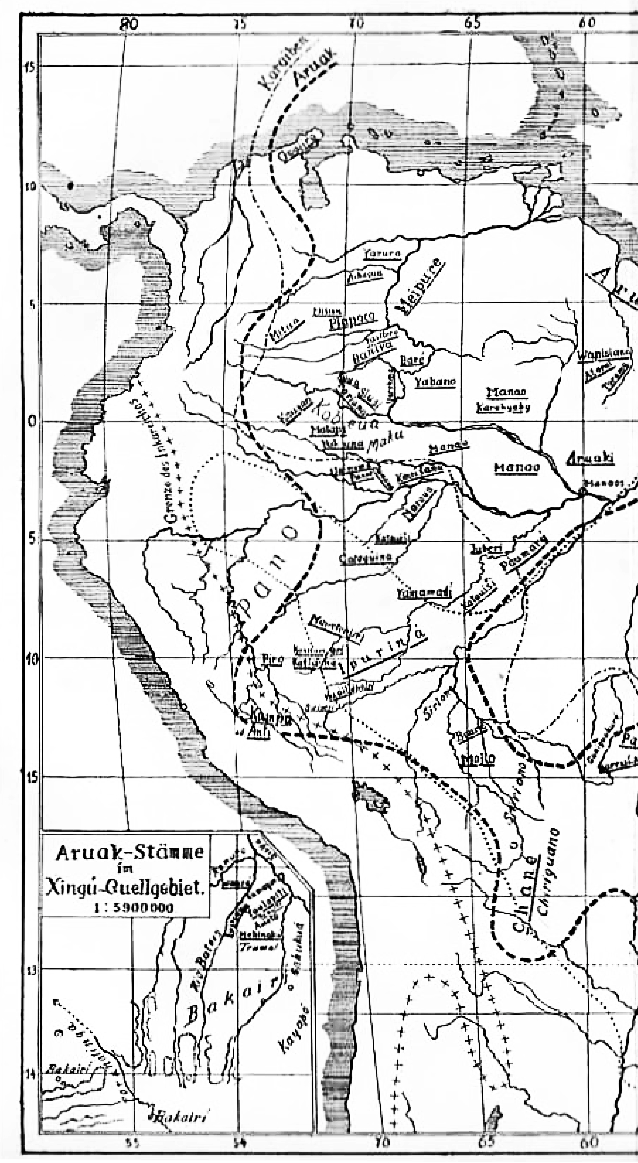
\includegraphics[width=\textwidth]{./MAPA_P1.pdf}  
 % \caption{Frontispício da primeira edição.}

\end{absolutelynopagebreak}
\end{figure}

\pagebreak
\thispagestyle{empty}

\begin{figure}[H]
\begin{absolutelynopagebreak}
\hspace*{-2cm}
  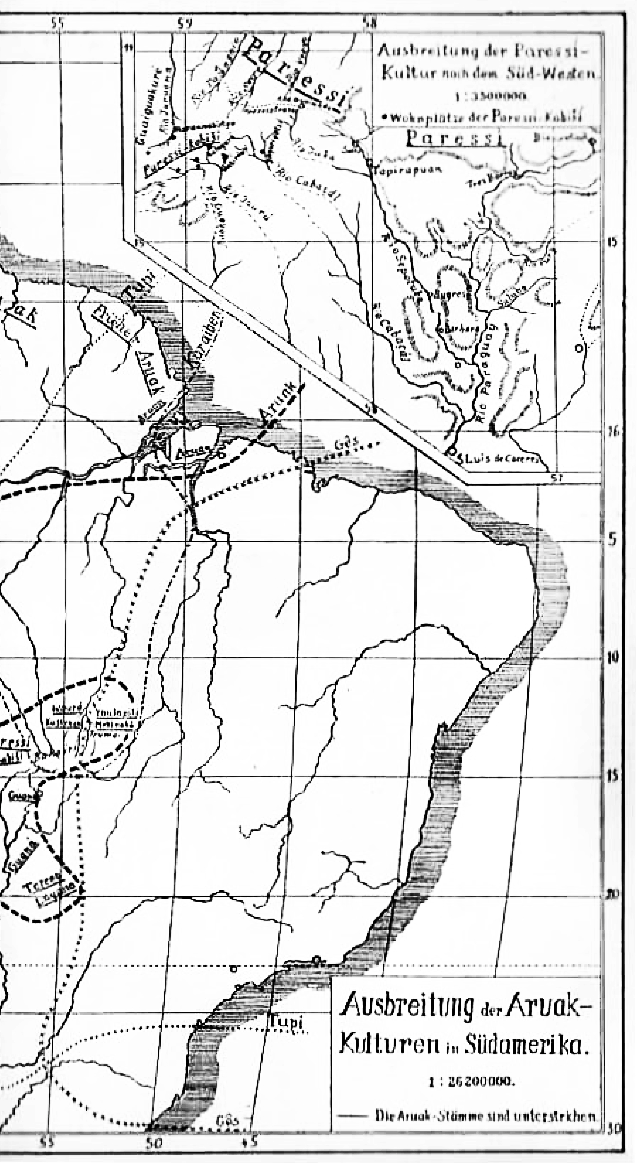
\includegraphics[width=\textwidth]{./MAPA_P2.pdf}  
  %\hfill
 % \caption{Frontispício da primeira edição.}

\end{absolutelynopagebreak}
\end{figure}
